\documentclass[a4paper,12pt]{article}

% Set margins
\usepackage[hmargin=2.5cm, vmargin=3cm]{geometry}

\frenchspacing

% Language packages
\usepackage[utf8]{inputenc}
\usepackage[T1]{fontenc}
\usepackage[magyar]{babel}

% AMS
\usepackage{amssymb,amsmath}

% Graphic packages
\usepackage{graphicx}

% Colors
\usepackage{color}
\usepackage[usenames,dvipsnames]{xcolor}

% \usepackage{plantuml}
% NOTE: Just ignore the content!
\usepackage{environ}
\NewEnviron{plantuml}{}{}

% Enumeration
\usepackage{enumitem}

% Links
\usepackage{hyperref}

\begin{document}

\begin{center}
	{\Large \textbf{Szakdolgozat bírálati folyamat és Záróvizsga menedzselő webalkalmazás - Specifikáció}}

	\bigskip
	
	{\large Drig Dávid}
\end{center}

\tableofcontents

\section{Bevezetés}

A dokumentum az elkészítendő webalkalmazás specifikációját tartalmazza.

\section{Szerepkörök}

A következő szakaszok a rendszer szereplőit, az általuk elérhető funkciókat, a szakdolgozat bírálati folyamat és a Záróvizsga során elvégzendő feladataikat tartalmazzák. Erről láthatunk egy áttekintést \aref{fig:use-cases}. ábrán.

\begin{figure}
	\centering
	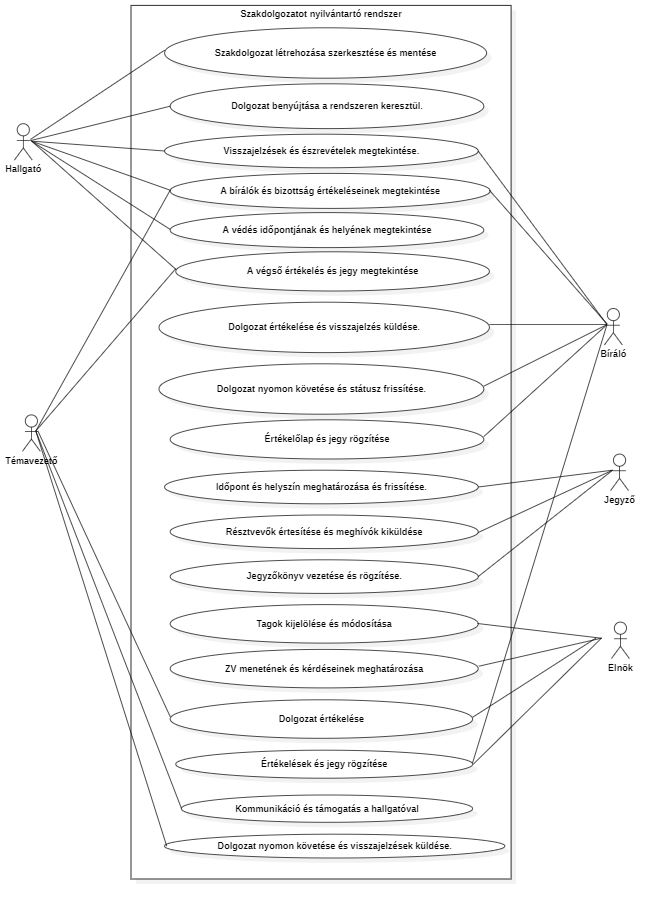
\includegraphics[width=\textwidth]{images/Use-case_diagram/use-case_1.jpg}
	\caption{Szerepkörök és használati esetek}
	\label{fig:use-cases}
\end{figure}

\subsection{Hallgató}

A hallgató, aki be szeretné nyújtani a szakdolgozatát, meg szeretné védeni, és záróvizsgázni szeretne.

\begin{itemize}
\item Szakdolgozat létrehozása, szerkesztése és mentése a rendszerben.
\item Az elkészült dolgozat benyújtása a rendszeren keresztül.
\item Visszajelzések és észrevételek megtekintése a dolgozatról a bírálók, témavezető vagy a bizottság részéről.
\item A bírálók és a bizottság értékeléseinek megtekintése.
\item A védés időpontjának és helyszínének megtekintése és kezelése.
\item A végső értékelés és jegy megtekintése.
\end{itemize}

\subsection{Bíráló}

A szakdolgozat szakmai elbírálására felkért külső bíráló.

\begin{itemize}
	\item A dolgozat értékelése és visszajelzés küldése a hallgatónak.
	\item A dolgozat nyomon követése és annak státuszának frissítése a rendszerben.
	\item Az értékelőlap és a végső jegy rögzítése a rendszerben.
\end{itemize}

\subsection{Jegyző}

A Záróvizsga jegyzője.

\begin{itemize}
	\item A záróvizsga időpontjának és helyszínének meghatározása és frissítése.
	\item A záróvizsga résztvevőinek (hallgató, bírálók, bizottság) értesítése és meghívók kiküldése.
	\item A záróvizsga jegyzőkönyvének vezetése és rögzítése a rendszerben.
\end{itemize}

\subsection{Elnök}

Záróvizsga bizottság elnöke:

\begin{itemize}
	\item A bizottság tagjainak kijelölése és módosítása.
	\item A záróvizsga menetének és a kérdéseknek meghatározása.
	\item A hallgató szakdolgozatának értékelése a bizottság véleménye alapján.
	\item A végső értékelés rögzítése a rendszerben.
\end{itemize}

\subsection{Témavezető}

A szakdolgozat témavezetője. (A konzulens a rendszerben csak névlegesen szerepel. Nem külön szerepkör.)

\begin{itemize}
	\item A hallgatóval való kommunikáció és támogatás a szakdolgozat elkészítése során.
	\item A hallgató dolgozatának nyomon követése és visszajelzések küldése.
	\item A bírálók és a bizottság értékeléseinek megtekintése.
	\item A végső értékelés és jegy rögzítése a rendszerben.
\end{itemize}

\section{Bírálati folyamat}

A következő szakaszokban a bírálati folyamat részletezését láthatjuk különféle szempontokból, szerepkörökből.

\subsection{Optimista eset}

A rendszer célja, hogy hatékonyan kezelje a szakdolgozatok Bírálati Folyamatát és a kapcsolódó érintett szereplők közötti kommunikációt. 

\begin{figure}
\centering
\begin{plantuml}
@startuml
title Bírálati folyamat (optimista eset)

Elnök->Hallgató: Felkérés regisztrációra
Hallgató->Elnök: Sikeres reg.
Elnök->Témavezető: Felkérés bírálatra
Témavezető->Bíráló: Felkérés bírálatra
Bíráló->Elnök: Bírálat
Témavezető->Elnök: Bírálat
@enduml
\end{plantuml}
\includegraphics[width=\textwidth]{images/review-optimistic}
\caption{Optimista eset}
\label{fig:review-optimistic}
\end{figure}

\Aref{fig:review-optimistic}. ábrán a leírás az alábbi lépéseket foglalja össze:
\begin{enumerate}
\item Elnök felkéri a Hallgatót a regisztrációra: A folyamatot az Elnök indítja, amikor felkéri a Hallgatót, hogy regisztráljon a rendszerbe. Ez a lépés azt jelenti, hogy a Hallgatónak lehetősége van hozzáférni a szakdolgozat bírálati folyamatához.

\item Hallgató sikeresen regisztrál: A Hallgató sikeresen regisztrál a rendszerbe, és így jogosultá válik a szakdolgozatának bírálati folyamatára.

\item Elnök felkéri a Témavezetőt a bírálatra: Az Elnök felkéri a Témavezetőt, hogy végezze el a szakdolgozat bírálatát. Ez a lépés azt jelzi, hogy a Témavezetőnek feladata van értékelni és észrevételeket tenni a szakdolgozatról.

\item Témavezető felkéri a Bírálót a bírálatra: A Témavezető felkéri a Bírálót, hogy részt vegyen a szakdolgozat bírálatában. A Bíráló feladata a szakdolgozat objektív értékelése és véleményezése.

\item Bíráló elküldi a bírálatot az Elnöknek: A Bíráló elkészíti a bírálatát a szakdolgozatról, és elküldi azt az Elnöknek. Ez a lépés azt jelenti, hogy a Bíráló megosztja az észrevételeit és értékelését a szakdolgozatról a rendszer adminisztrátorával.

\item Témavezető elküldi a bírálatot az Elnöknek: A Témavezető szintén elkészíti a saját bírálatát a szakdolgozatról, és azt az Elnöknek küldi el. Ez a lépés lehetővé teszi, hogy mind a Témavezető, mind a Bíráló észrevételeit összevetve az Elnök döntést hozzon a szakdolgozattal kapcsolatban.
\end{enumerate}

\subsection{Többszörös bírálói felkérés}

Ez a szekvenciadiagram lépésről lépésre bemutatja a Többszörös Bírálói Felkérés Folyamatát, a felkéréstől a végleges bírálati visszajelzésig.

\begin{figure}
\centering
\begin{plantuml}
@startuml
title Többszörös bírálói felkérés folyamata

participant Elnök as E
participant Hallgató as H
participant Témavezető as T
participant Bíráló as B

E->H: Felkérés regisztrációra
H->E: Sikeres regisztráció
E->T: Felkérés bírálatra
T->B: Felkérés bírálatra

loop Több bíráló
	alt Felkérés elfogadva
		note left of B 
		Elfogadva
		end note
	else Felkérés visszautasítva
		note left of B 
		Visszautasítva
		end note
	end
end

note right of T 
Visszajelzés a bírálókról
end note

T -> E: Bírálat
B -> E: Bírálat
@enduml
\end{plantuml}
\includegraphics[width=\textwidth]{images/review-multiple}
\caption{Több bíráló felkérése}
\label{fig:review-multiple}
\end{figure}

A leírás (\ref{fig:review-multiple}. ábra) az alábbi lépéseket foglalja össze:

\begin{enumerate}
\item Felkérés a regisztrációra: A folyamatot az Elnök indítja, amikor felkéri a Hallgatót, hogy regisztráljon a rendszerbe. Ez a lépés azt jelenti, hogy a Hallgatónak lehetősége van hozzáférni a szakdolgozat bírálati folyamatához.

\item Hallgató sikeresen regisztrál: A Hallgató sikeresen regisztrál a rendszerbe, és így jogosultá válik a szakdolgozatának bírálati folyamatára.

\item Elnök felkéri a Témavezetőt a bírálatra: Az Elnök felkéri a Témavezetőt, hogy végezze el a szakdolgozat bírálatát. Ez a lépés azt jelzi, hogy a Témavezetőnek feladata van értékelni és észrevételeket tenni a szakdolgozatról.

\item Témavezető felkéri a Bírálót a bírálatra: A Témavezető felkéri a Bírálót, hogy részt vegyen a szakdolgozat bírálatában. A Bíráló feladata a szakdolgozat objektív értékelése és véleményezése.

\item Elfogadás: A Bíráló elfogadja a felkérést, és ezt jelzi.

\item Visszautasítás: A Bíráló visszautasítja a felkérést, és ezt jelzi.

\item Visszajelzés a bírálókról: A Témavezető visszajelzést ad az Elnöknek a bírálók elfogadásáról vagy visszautasításáról.

\item Bíráló elküldi a bírálatot az Elnöknek: A Bíráló elkészíti a bírálatát a szakdolgozatról, és elküldi azt az Elnöknek. Ez a lépés azt jelenti, hogy a Bíráló megosztja az észrevételeit és értékelését a szakdolgozatról a rendszer adminisztrátorával.

\item Témavezető elküldi a bírálatot az Elnöknek: A Témavezető szintén elkészíti a saját bírálatát a szakdolgozatról, és azt az Elnöknek küldi el. Ez a lépés lehetővé teszi, hogy mind a Témavezető, mind a Bíráló észrevételeit összevetve az Elnök döntést hozzon a szakdolgozattal kapcsolatban.
\end{enumerate}

\subsection{Hallgatók felvitele}

Ez a szekvenciadiagram (\ref{fig:student-creation-process}. ábra) részletesen szemlélteti a Hallgatók felvitele folyamatát az adatok megadásától az adatlap jóváhagyásának értesítéséig, mindezt az Elnök, Hallgató és Jegyző közötti interakciókkal.

\begin{figure}
	\centering
	\begin{plantuml}
@startuml
title Hallgatók felvitele - Szekvenciadiagram

participant Elnök as E
participant Hallgató as H
participant Jegyző as J

note over E
Hallgatói adatok megadása
end note
note over E
Adatok ellenőrzése és validáció
end note

E->>H: Felvételre kerültél!

note over H 
Belépés a rendszerbe
end note

note over H 
Adatlap kitöltése
end note

H-->J: Új adatlap

note over J 
Új adatlap érkezett
end note

note over J 
Adatlap ellenőrzése
end note

J->>H: Visszajelzés (ha szükséges)

note over J 
Adatlap jóváhagyása
end note

note over J 
Jóváhagyott adatok rögzítése
end note

J-->>E: Adatlap jóváhagyva értesítés

E-->>H: Adatlap jóváhagyva értesítés
@enduml
	\end{plantuml}
	\includegraphics[width=\textwidth]{images/student-creation-process}
	\caption{Hallgatók létrehozásának a folyamata}
	\label{fig:student-creation-process}
\end{figure}

\begin{enumerate}
\item Hallgató adatok megadása: Az Elnök megadja a Hallgató adatait a rendszerben, hogy felkészüljenek a regisztrációra. Az adatok tartalmazzák a szükséges információkat a Hallgatóról.

\item Adatok ellenőrzése és validáció: Az Elnök ellenőrzi és érvényesíti az adatokat, hogy biztos legyen a hitelességükben és a pontosságukban.

\item Felvételre kerülés értesítése: Az Elnök értesíti a Hallgatót a sikeres felvételről, és arról, hogy részt vehet a folyamatban.

\item Belépés a rendszerbe: A Hallgató belép a rendszerbe a saját fiókjába, hogy folytassa a felvételi folyamatot.

\item Adatlap kitöltése: A Hallgató kitölti az adatlapját a szükséges információkkal.

\item Új adatlap értesítése: A Hallgató elküldi az újonnan kitöltött adatlapot a Jegyzőnek, jelezve a további folyamat kezdetét.

\item Adatlap ellenőrzése: A Jegyző értesül arról, hogy új adatlap érkezett, majd alaposan ellenőrzi az adatokat és a kitöltött információkat.

\item Visszajelzés és jóváhagyás: A Jegyző visszajelzést küld a Hallgatónak az adatlap jóváhagyásáról, és esetleges korrekciókról, ha szükséges.

\item Adatlap jóváhagyása: Miután az adatlapot jóváhagyásra alkalmasnak találták, a Jegyző hivatalosan is jóváhagyja az adatlapot.

\item Értesítés a jóváhagyásról: A Jegyző értesíti az Elnököt az adatlap jóváhagyásáról és a felvétel sikerességéről.

\item Adatlap jóváhagyásának értesítése a Hallgatónak: Az Elnök értesíti a Hallgatót az adatlap jóváhagyásáról és a felvétel megerősítéséről.
\end{enumerate}

\subsection{Témavezető bírálati folyamat}

A folyamatábra bemutatja a szakdolgozat bírálat feltöltésének folyamatát a Témavezető és a Bíráló között (\ref{fig:Biralat_Feltoltes}. ábra).

\begin{figure}
\centering
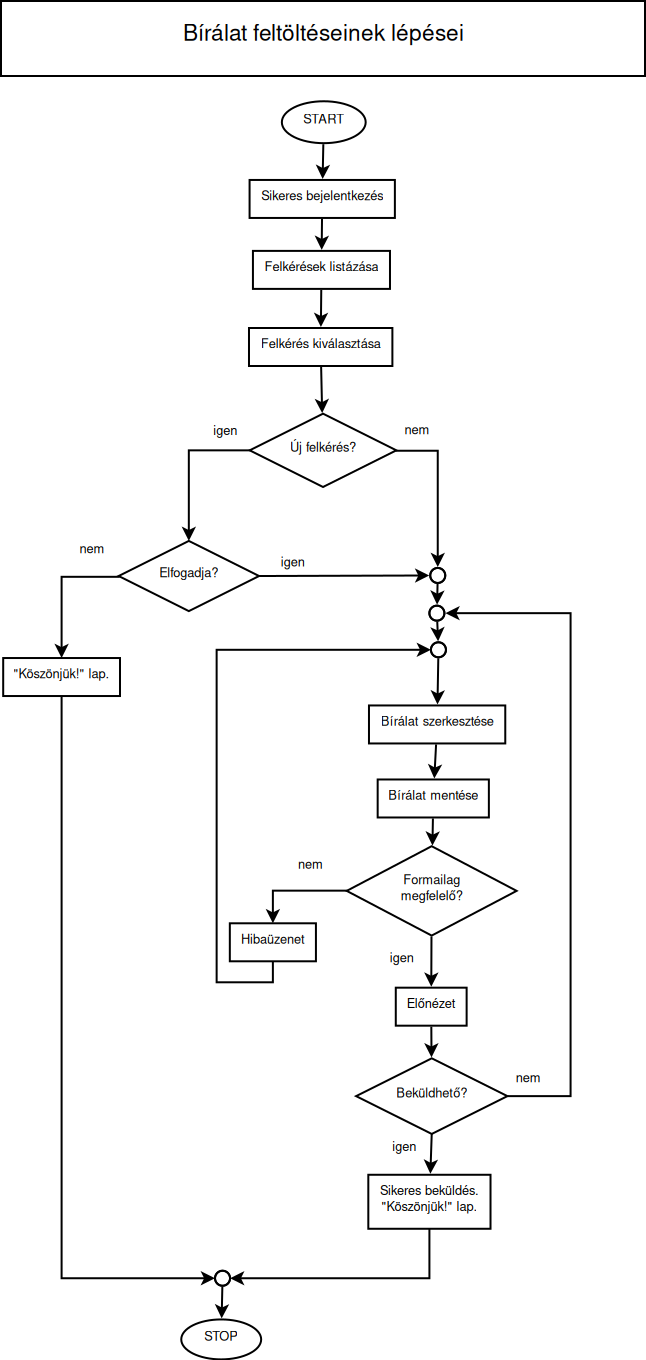
\includegraphics[scale=0.45]{images/Folyamatabra/Biralat_Feltoltes.png}
\caption{Bírálat feltöltés folyamata}
\label{fig:Biralat_Feltoltes}
\end{figure}

\begin{enumerate}
\item A Témavezető és a Bíráló bejelentkezik: A Témavezető és a Bíráló is bejelentkezik a rendszerbe, hogy hozzáférjenek a szükséges funkciókhoz.

\item Témavezető kilistázza és kiválasztja a Bírálót: A Témavezető megjeleníti a rendszerben elérhető Bírálók listáját és a Témavezető kiválasztja a Bírálót.

\item Felhasználók kiválasztják a szakdolgozatot: Mind a Témavezető, mind a Bíráló kiválasztja a szakdolgozatot, amelyre a bírálatot el szeretné készíteni.

\item A Felhasználók megírják a bírálatot: Mind a Témavezető, mind a Bíráló megírja a bírálatot.

\item Bírálat mentése és feldolgozása a rendszerben: A rendszer elmenti és feldolgozza a feltöltött bírálatot.

\item Rendszer ellenőrzi, hogy a bírálat PDF formátumban van és érvényes-e: A rendszer ellenőrzi, hogy a bírálat valóban PDF formátumban van-e és érvényes-e.

\item Rendszer előnézetet készít a bírálatból: A rendszer előnézetet készít a bírálatból, hogy a Témavezető és a Bíráló ellenőrizhesse a dokumentumot.

\item Témavezető szerkeszti a bírálatot (szükség esetén): A Témavezető lehetősége van szerkeszteni a bírálatot, ha szükségesnek látja.

\item Bíráló szerkeszti a bírálatot (szükség esetén): A Bírálónak is lehetősége van szerkeszteni a bírálatot, ha szükségesnek tartja.

\item Bírálat véglegesítése és mentése a rendszerben: A Témavezető és a Bíráló véglegesíti a szerkesztéseket, majd a rendszer elmenti a végleges bírálatot.

\item Visszajelzés a rendszerben a Témavezetőnek és a Bírálónak: A rendszer visszajelzést küld mind a Témavezetőnek, mind a Bírálónak arról, hogy a bírálatuk sikeresen rögzítésre került.

\item Témavezető és a Bíráló megtekinti a bírálatot: Végül mind a Témavezető, mind a Bíráló megtekinti a véglegesített bírálatot a rendszerben.
\end{enumerate}

\section{Lapok részletezése}

\subsection{Bejelentkezés (Login)}

\begin{figure}
	\centering
	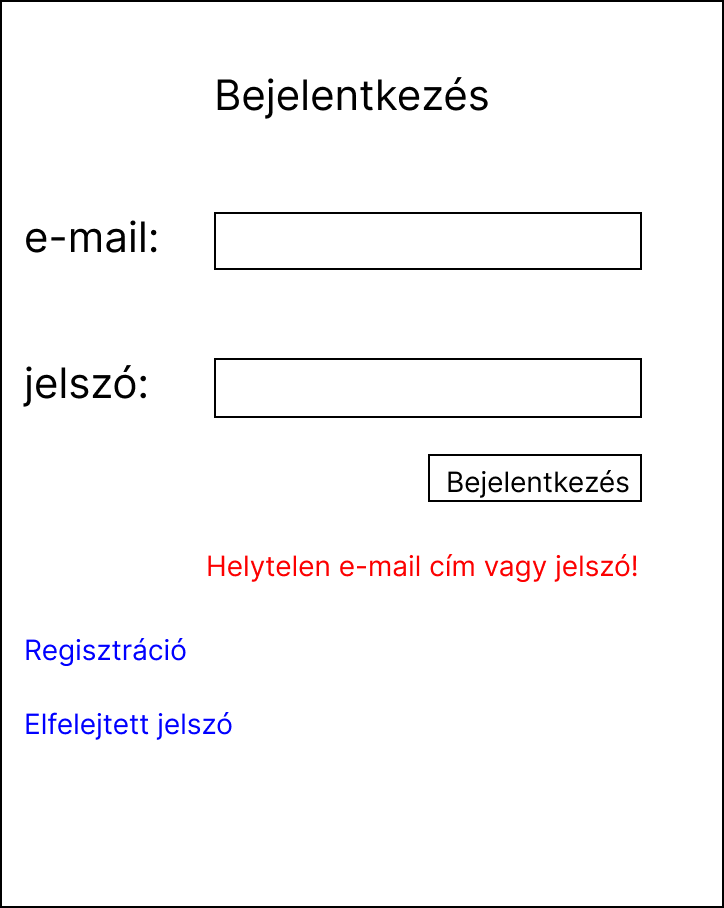
\includegraphics[width=\textwidth]{images/Web_pages/Login.jpg}
	\caption{}
	\label{fig:Login}
\end{figure}

\begin{itemize}
	\item A hibamező a hiányzó e-mail címet és/vagy jelszót jelzi.
	\item A hibaüzenet egy bejelentkezési próba után jelenik meg, amikor az e-mail-jelszó pár érvénytelen.
\end{itemize}

Lehetséges hibaüzenetek:
\begin{itemize}
	\item Az e-mail cím hiányzik!
	\item Hiányzik a jelszó!
	\item Az e-mail cím vagy a jelszó érvénytelen!
\end{itemize}

Sikeres bejelentkezés után megnyílik a felhasználó irányítópult-oldala.

\subsection{Regisztráció (Registration)}

\begin{figure}
	\centering
	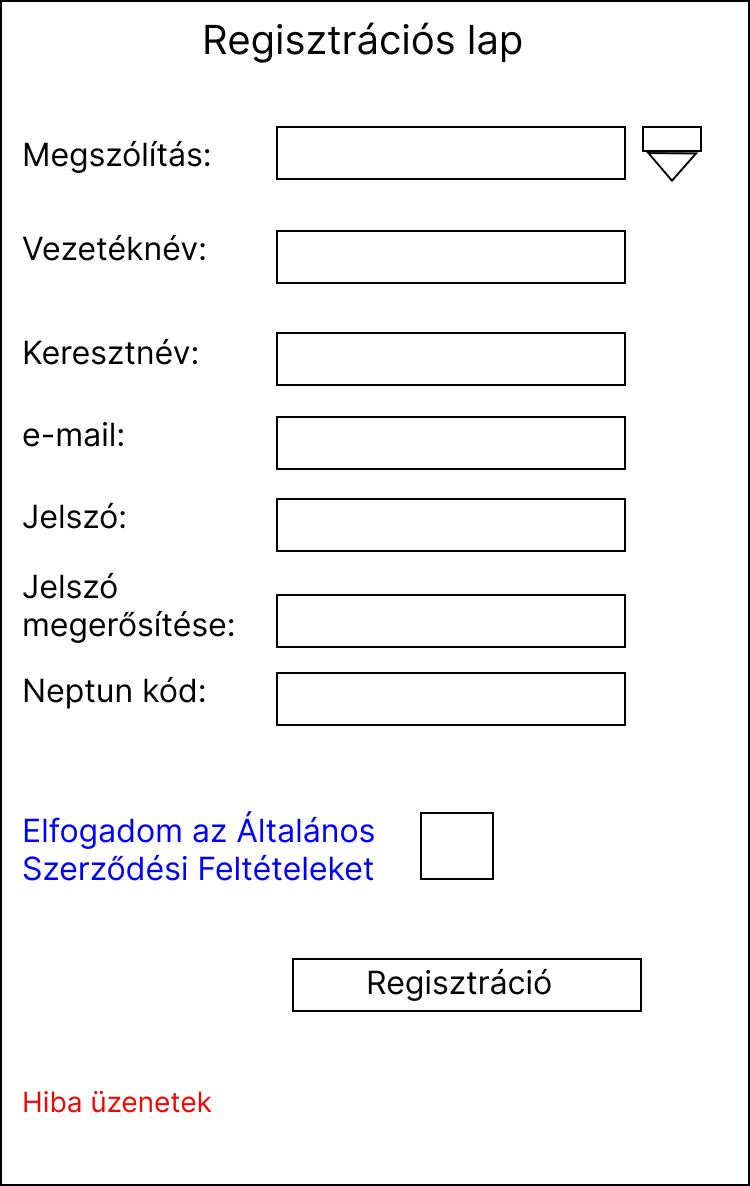
\includegraphics[width=\textwidth]{images/Web_pages/Registration.jpg}
	\caption{}
	\label{fig:Registration}
\end{figure}

\begin{itemize}
	\item A cím kivételével minden mező kitöltése kötelező.
	\item Hibaüzenet jelenik meg minden érvénytelen adatnál (a regisztrációs próba után).
	\item A helyreállítási link akkor jelenik meg, ha az e-mail cím már létezik.
\end{itemize}

Lehetséges hibaüzenetek:
\begin{itemize}
	\item A keresztnév hiányzik!
	\item A családnév hiányzik!
	\item Az e-mail cím hiányzik!
	\item Az e-mail cím formátuma érvénytelen!
	\item A megadott e-mail cím már használatban van!
	\item A feltételek elfogadása nélkül nem regisztrálhat!
\end{itemize}

Sikeres regisztráció után megnyílik a felhasználó irányítópult-oldala.

\subsection{Elfelejtett jelszó (Forgotten\_Password)}

\begin{figure}
	\centering
	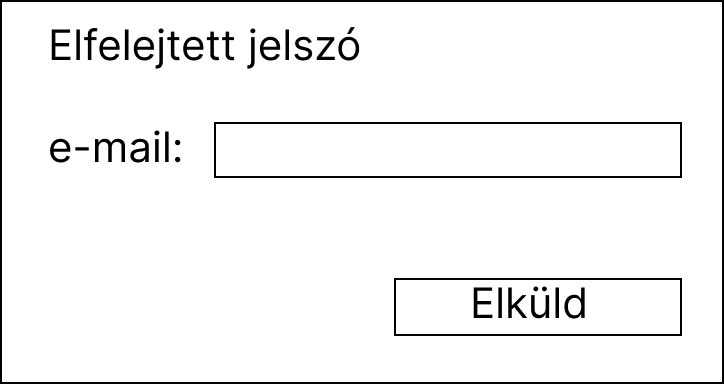
\includegraphics[width=\textwidth]{images/Web_pages/Forgotten_Password.jpg}
	\caption{}
	\label{fig:Forgotten_Password}
\end{figure}

Az Elküld gomb megnyomása után az alábbi üzenetek egyike jelenik meg.

\begin{itemize}
	\item Egy e-mailt küldtünk a sample@address.com e-mail címre.
	\item Az e-mail cím formátuma érvénytelen!
	\item A sample@address.com e-mail cím nincs regisztrálva a Szerkesztői rendszerben.
	\item Hiba történt, miközben a rendszer megpróbálta elküldeni az e-mailt. Kérjük, próbálja újra később.
\end{itemize}

Sikeres e-mail küldés után a szövegbeviteli mező és a gomb eltűnik.

\subsection{Hallgatók felvitele (Enrollment\_of\_students)}

\begin{figure}
	\centering
	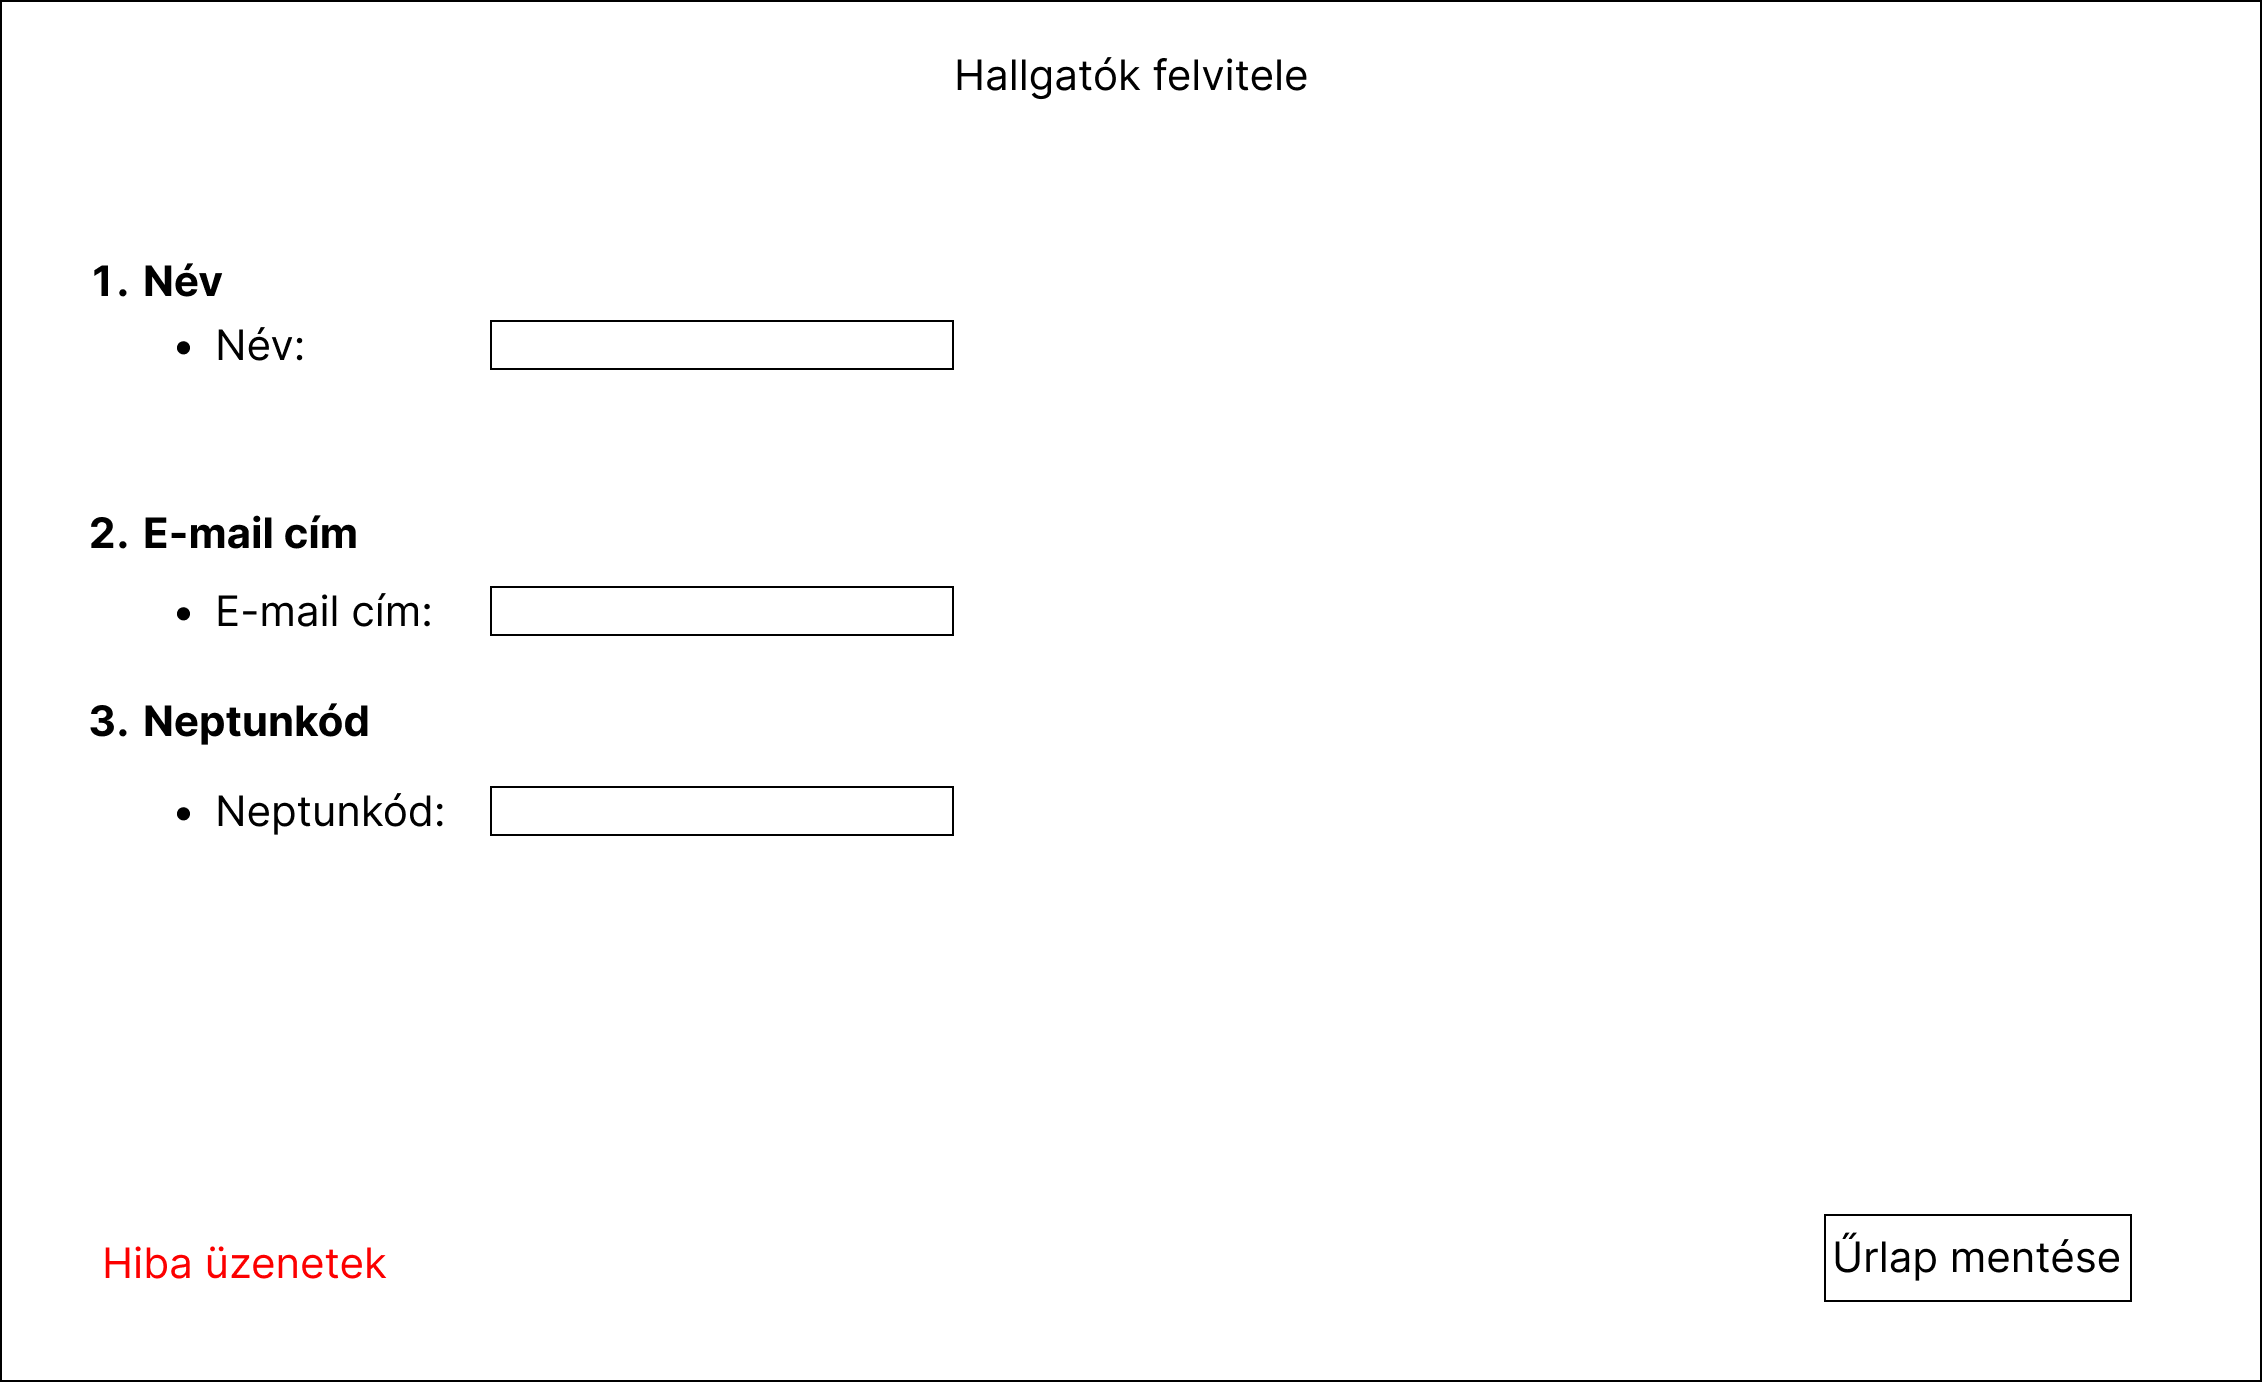
\includegraphics[width=\textwidth]{images/Web_pages/Enrollment_of_students.png}
	\caption{}
	\label{fig:Enrollment_of_students}
\end{figure}

\subsection{Szakdolgozatok listázása (Thesis\_List)}

\begin{figure}
	\centering
	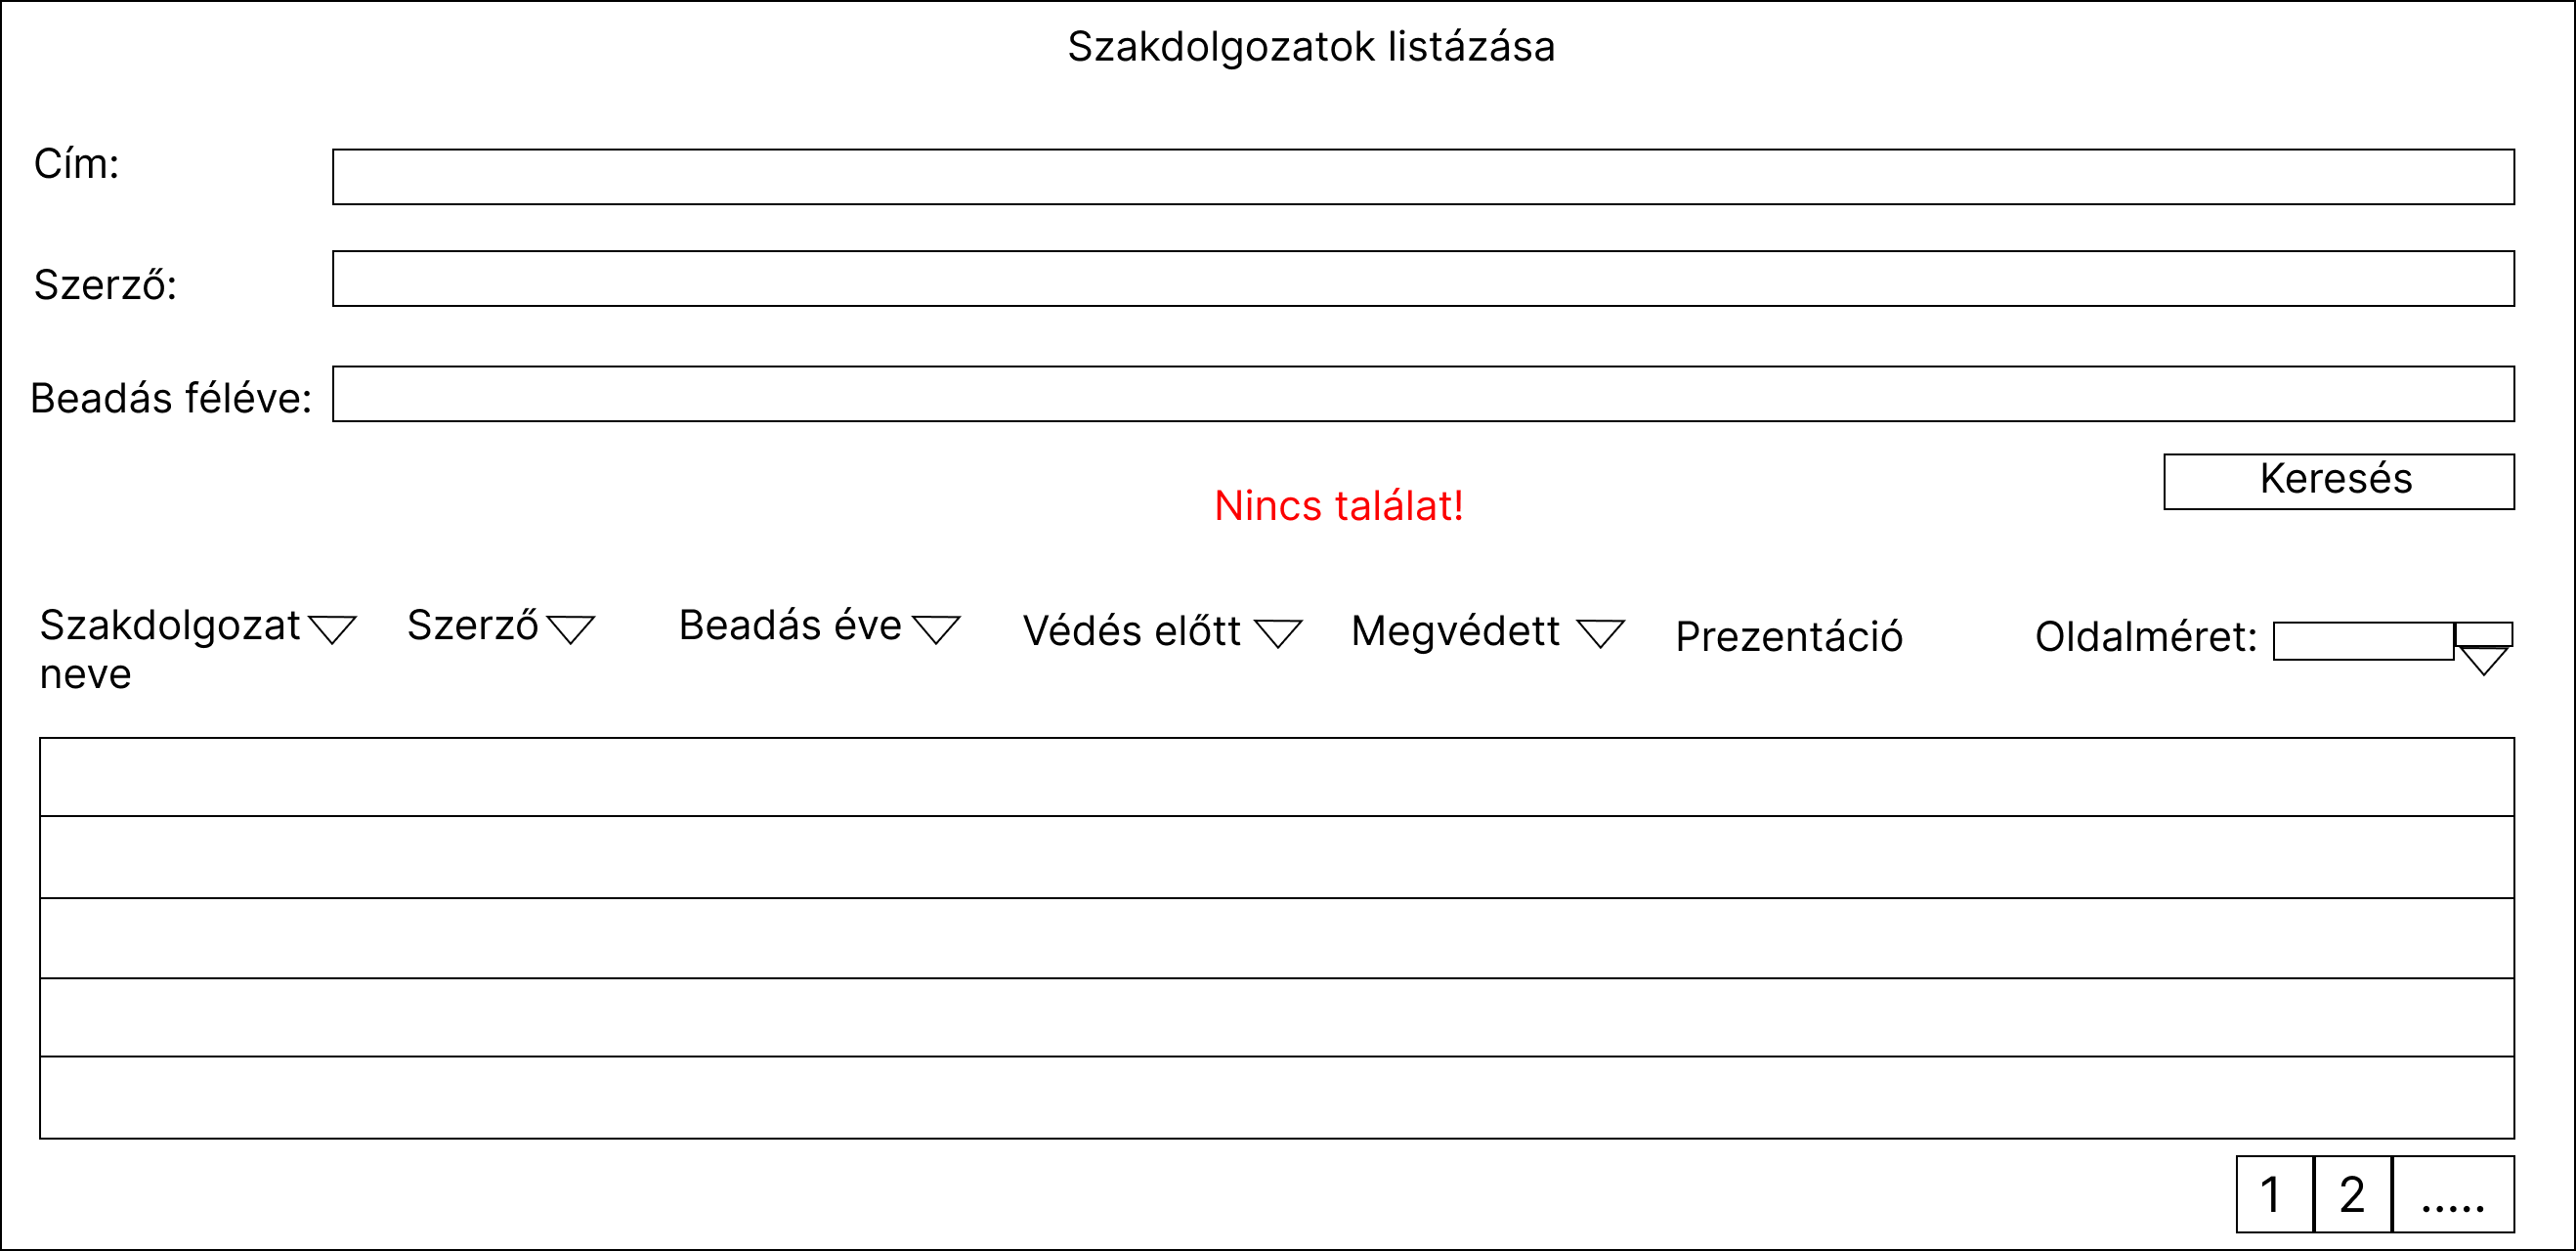
\includegraphics[width=\textwidth]{images/Web_pages/Thesis_List.jpg}
	\caption{}
	\label{fig:Thesis_List}
\end{figure}

A weblap a szakdolgozatok listázását mutatja.

\begin{itemize}
	\item A hiba üzenet akkor jelenik meg ha a felhaszáló nem ad meg adatot illetve ha a felhasználó téves adatokat ad meg.
\end{itemize}

\subsubsection{Szakdolgozat részletei (Thesis\_Details)}

\begin{figure}
	\centering
	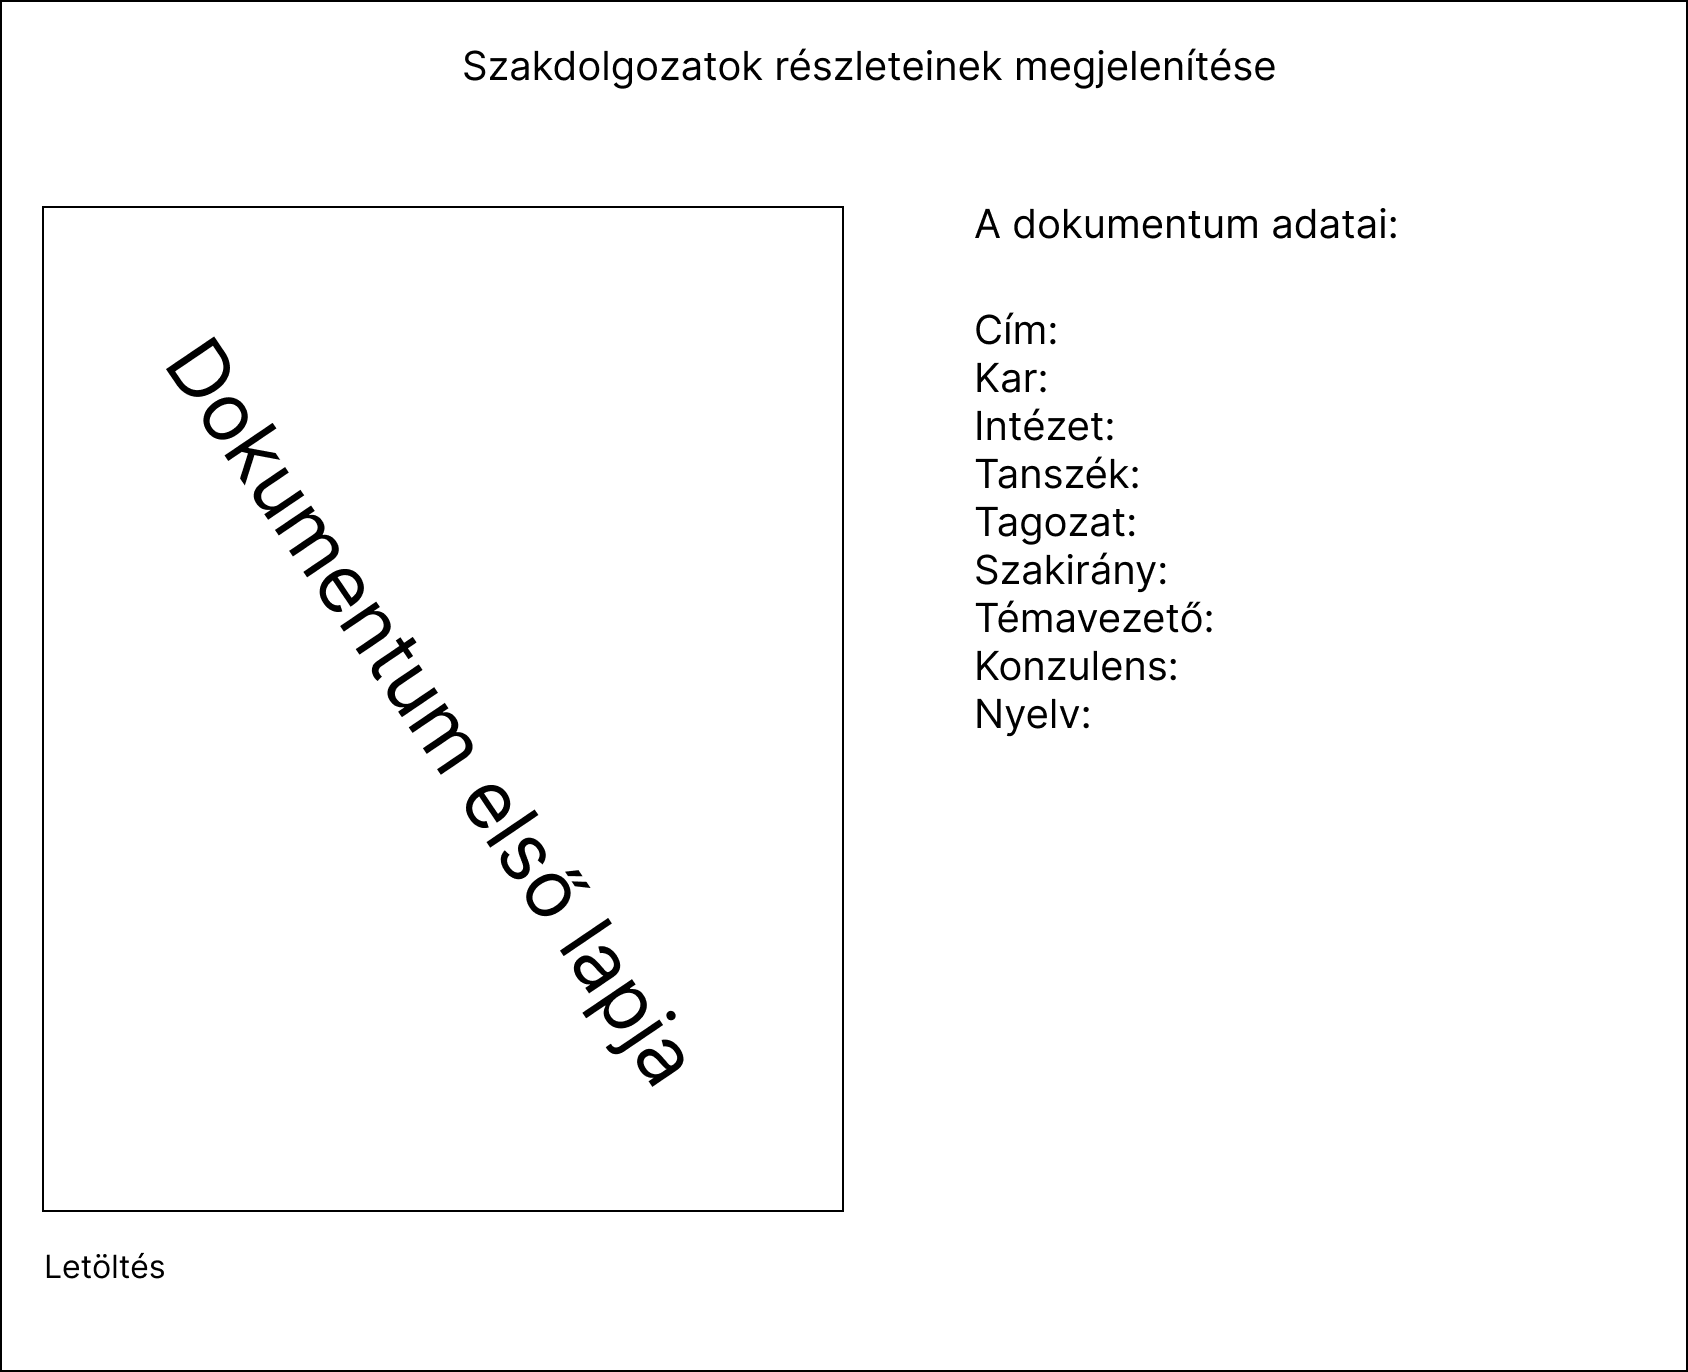
\includegraphics[width=\textwidth]{images/Web_pages/Thesis_Details.jpg}
	\caption{}
	\label{fig:Thesis_Details}
\end{figure}

A weblap egy adott szakdolgozat részleteit jeleníti meg. A lapot a *Szakdolgozatok listázása* lapból érhetjük el. 

\subsection{Szakdolgozat feltöltése}

A folyamat több lapból áll melyek átsegítik a felhasználót a szakdolgozat feltöltésében.

\subsubsection{Alapadatok (Title\_Settings)}

\begin{figure}
	\centering
	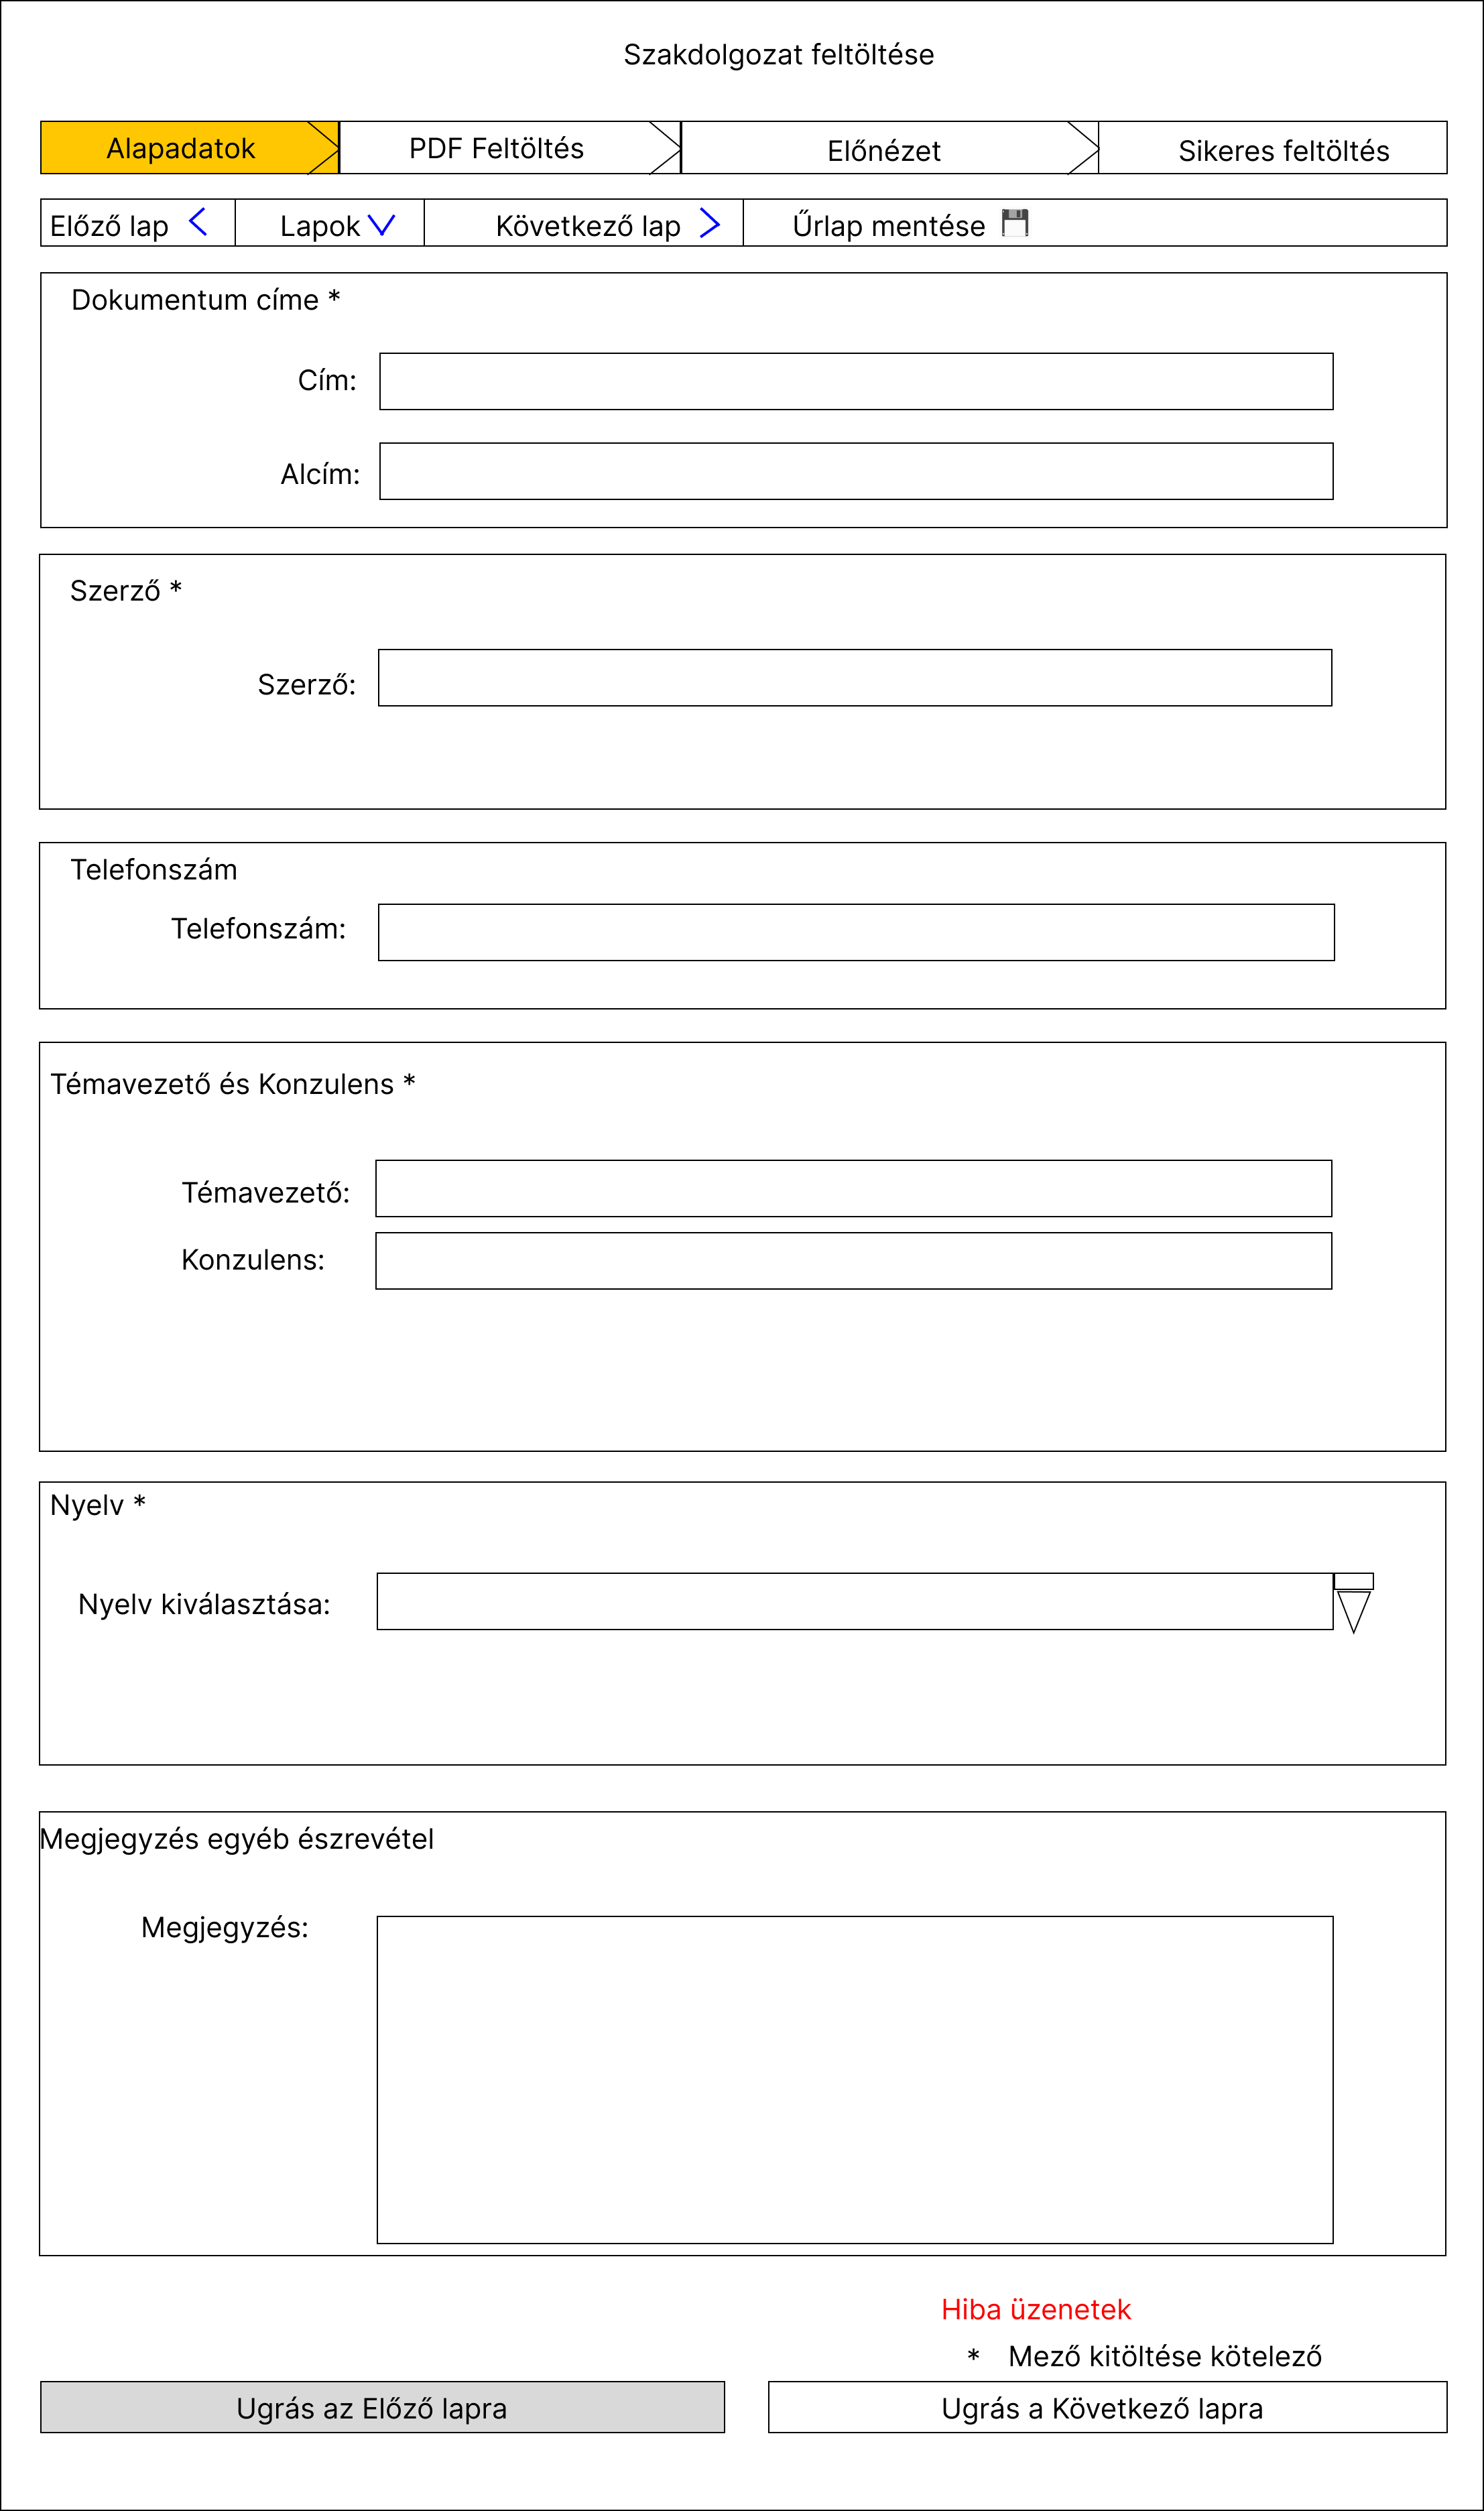
\includegraphics[width=\textwidth]{images/Web_pages/Title_Settings.png}
	\caption{}
	\label{fig:Title_Settings}
\end{figure}

Lehetséges hibaüzenetek:
\begin{itemize}
	\item Nem töltöttél ki minden fontosabb mezőt.
	\item Mielőtt tovább lépsz kérlek mentsd az oldalt.
\end{itemize}

\subsubsection{PDF Feltöltés (PDF\_Upload)}

\begin{figure}
	\centering
	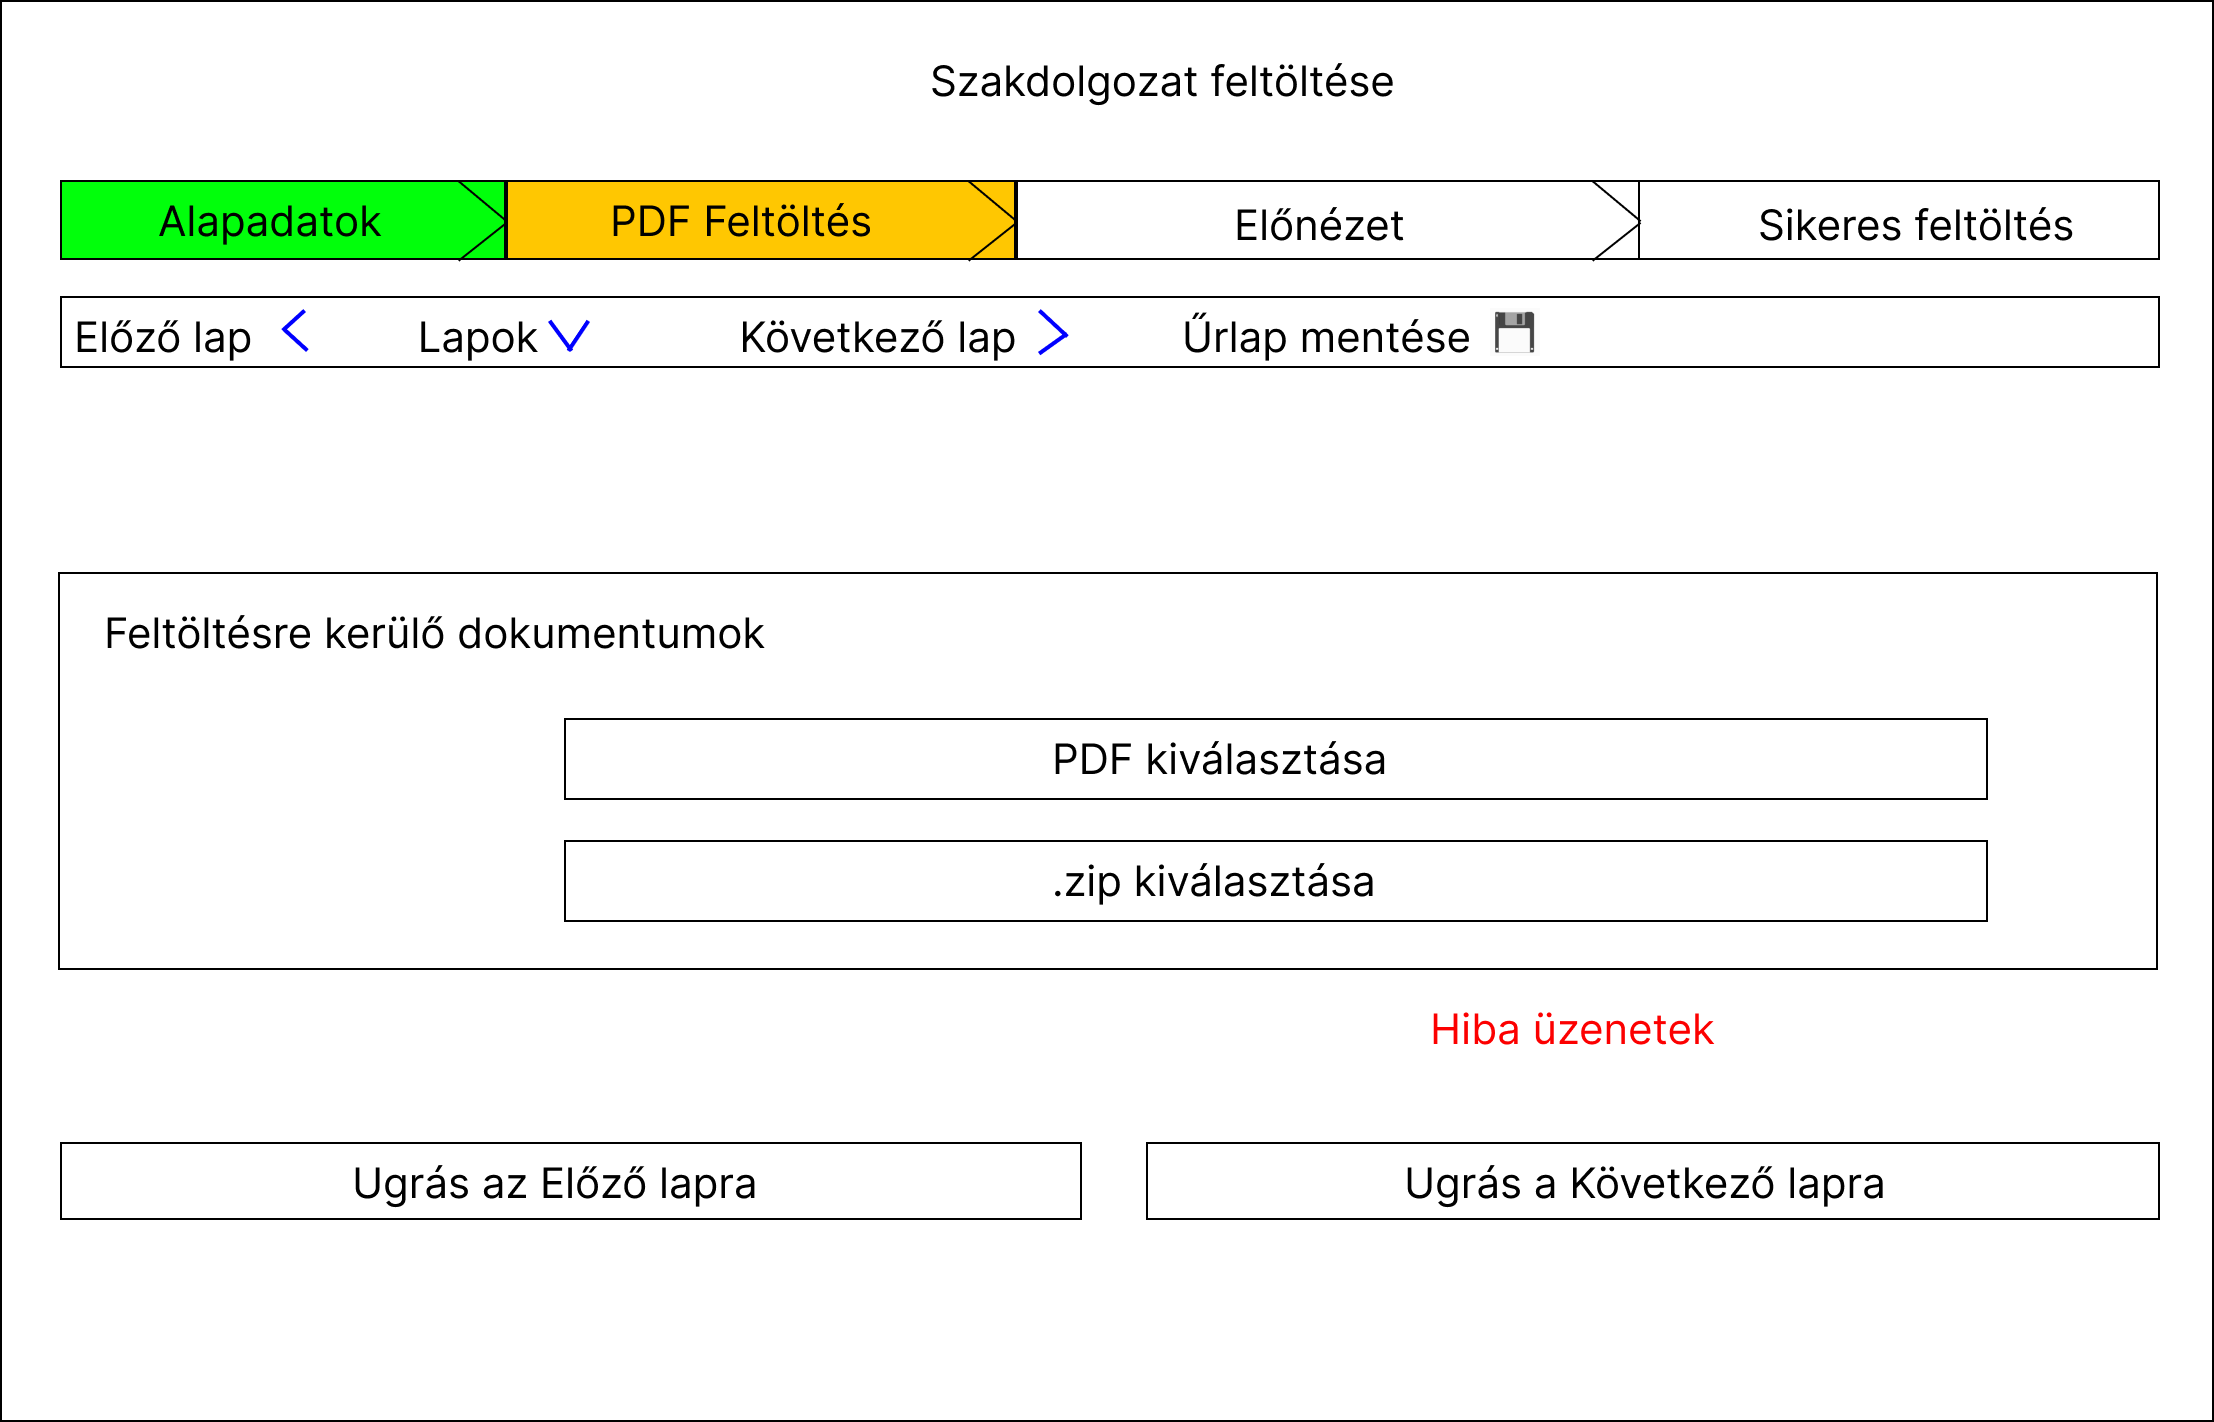
\includegraphics[width=\textwidth]{images/Web_pages/PDF_Upload.jpg}
	\caption{}
	\label{fig:PDF_Upload}
\end{figure}

Lehetséges hibaüzenetek:
\begin{itemize}
	\item A fájl mérete túl nagy
	\item A fájl nem a megfelelő formátumban van
\end{itemize}

\subsubsection{Előnézet (Preview)}

\begin{figure}
	\centering
	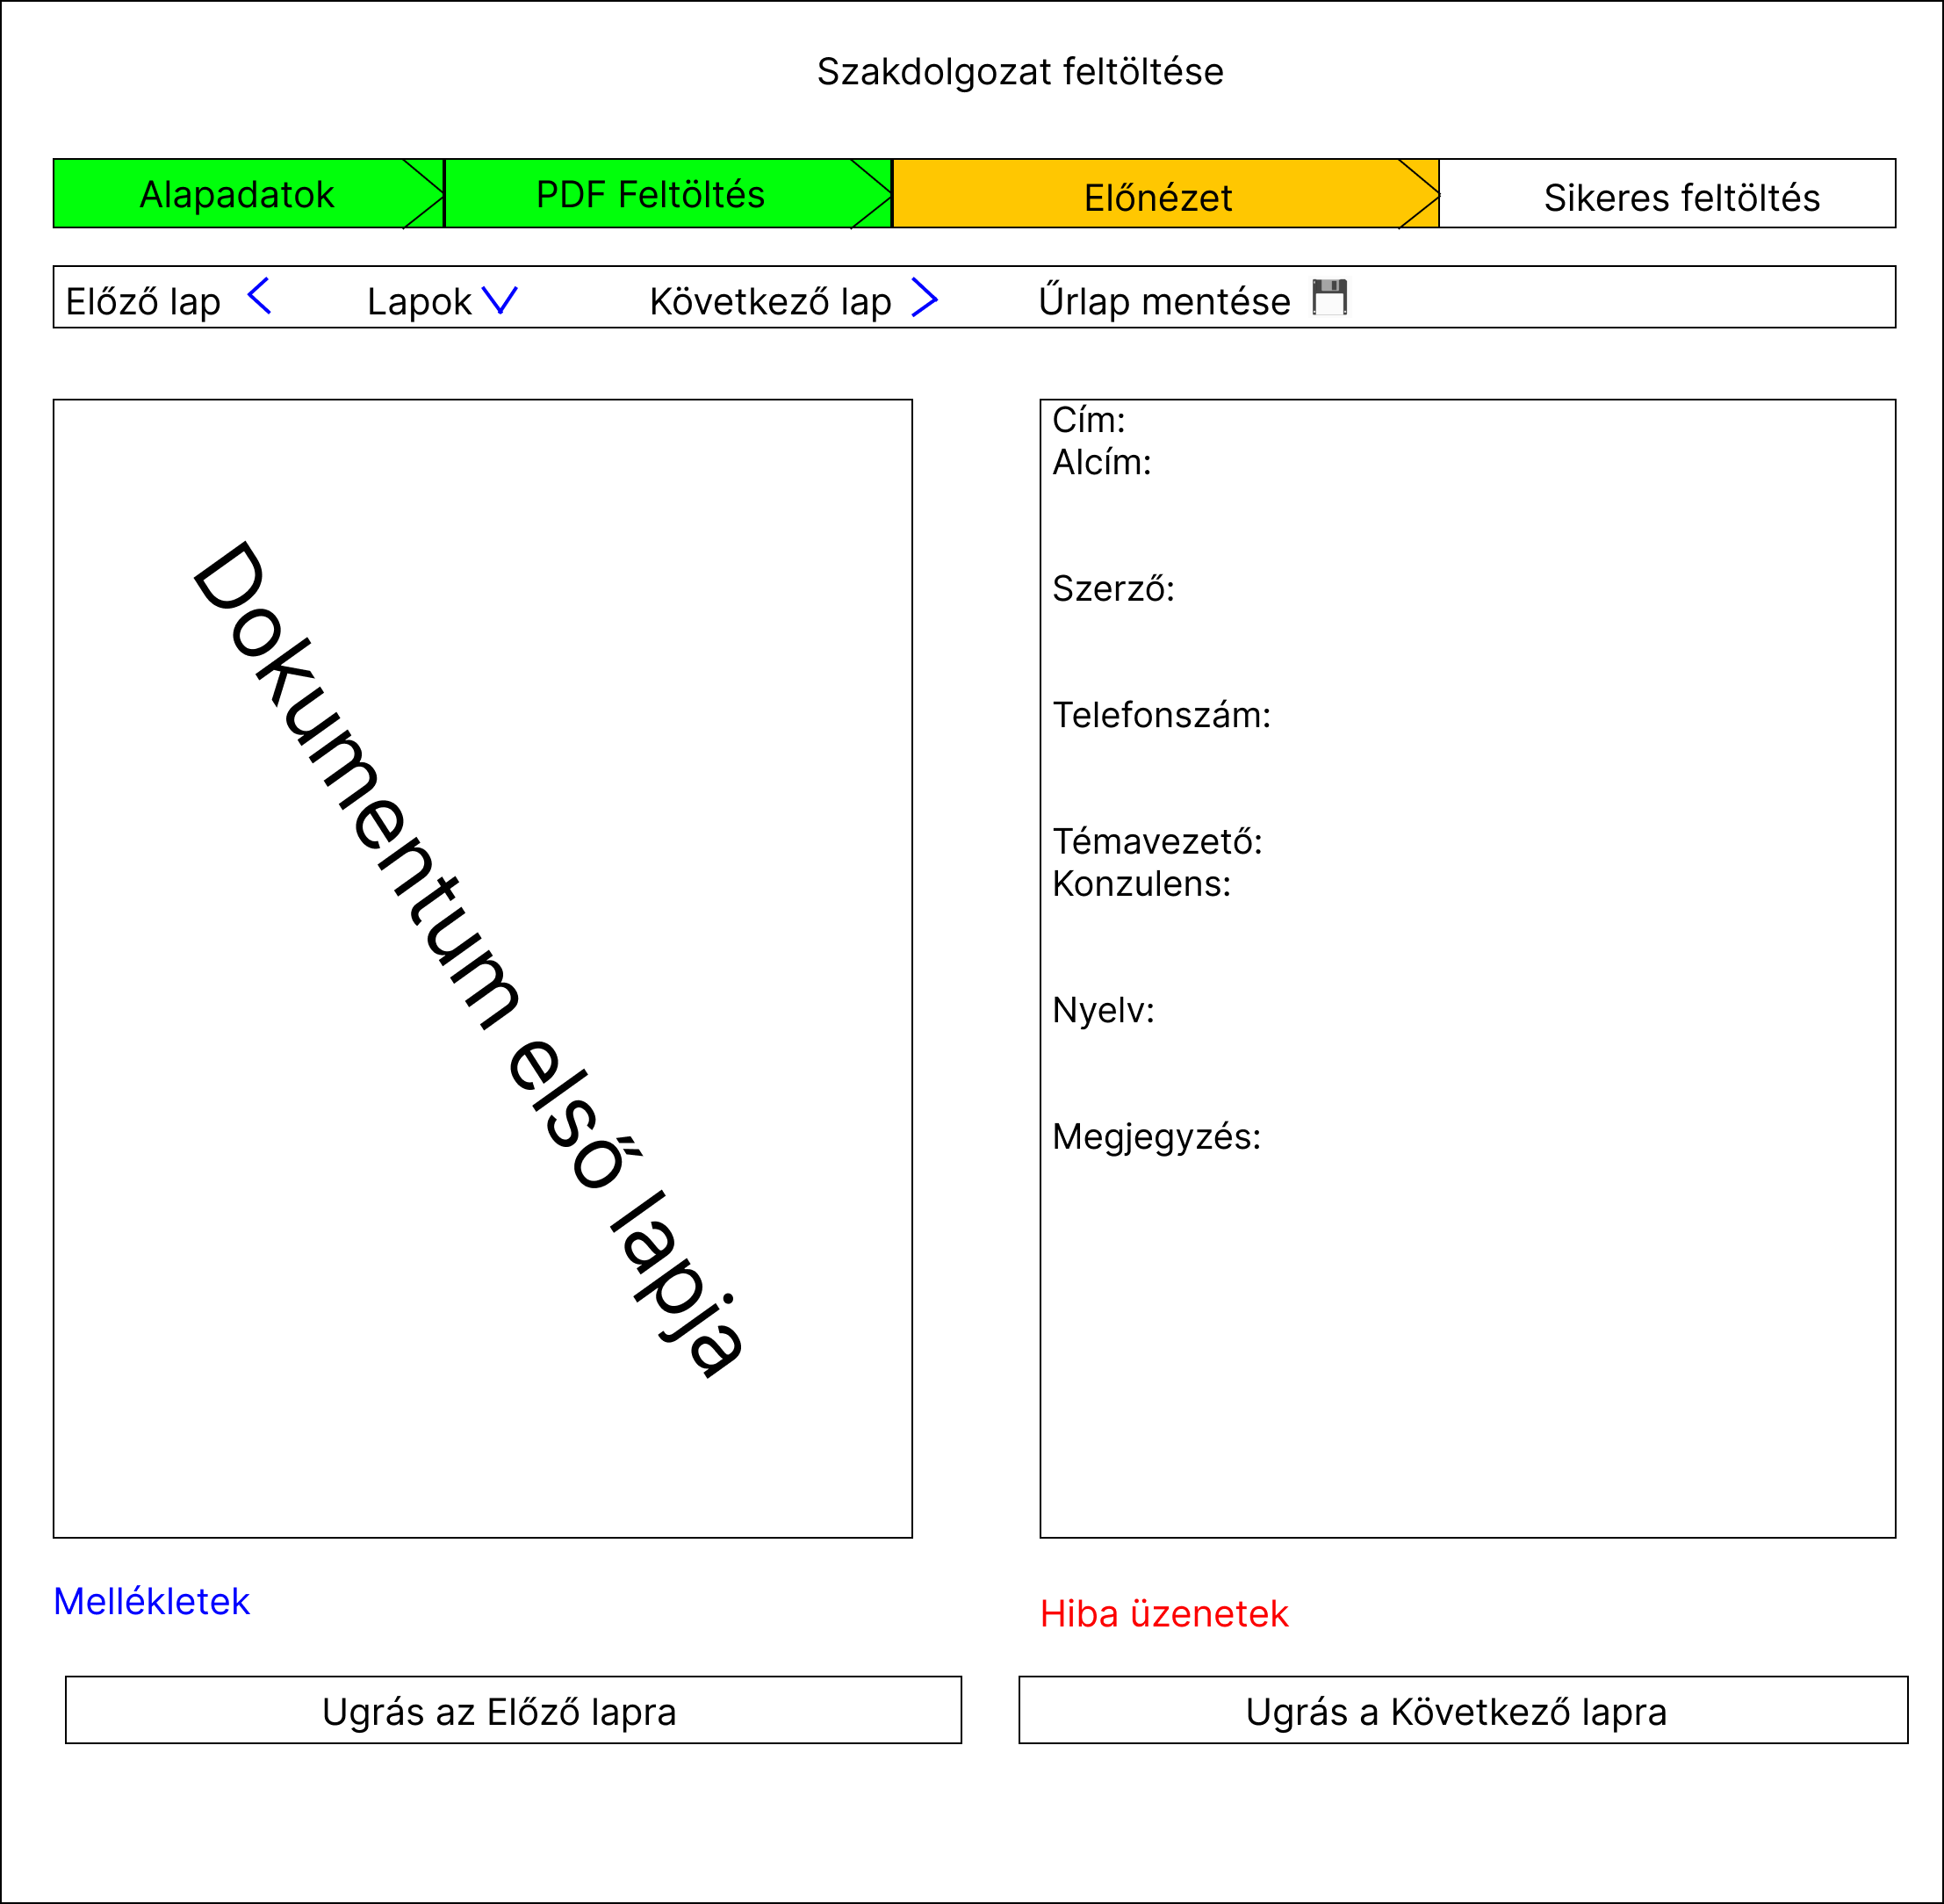
\includegraphics[width=\textwidth]{images/Web_pages/Preview.jpg}
	\caption{}
	\label{fig:Preview}
\end{figure}

\subsubsection{Sikeres feltöltés (Completed)}

\begin{figure}
	\centering
	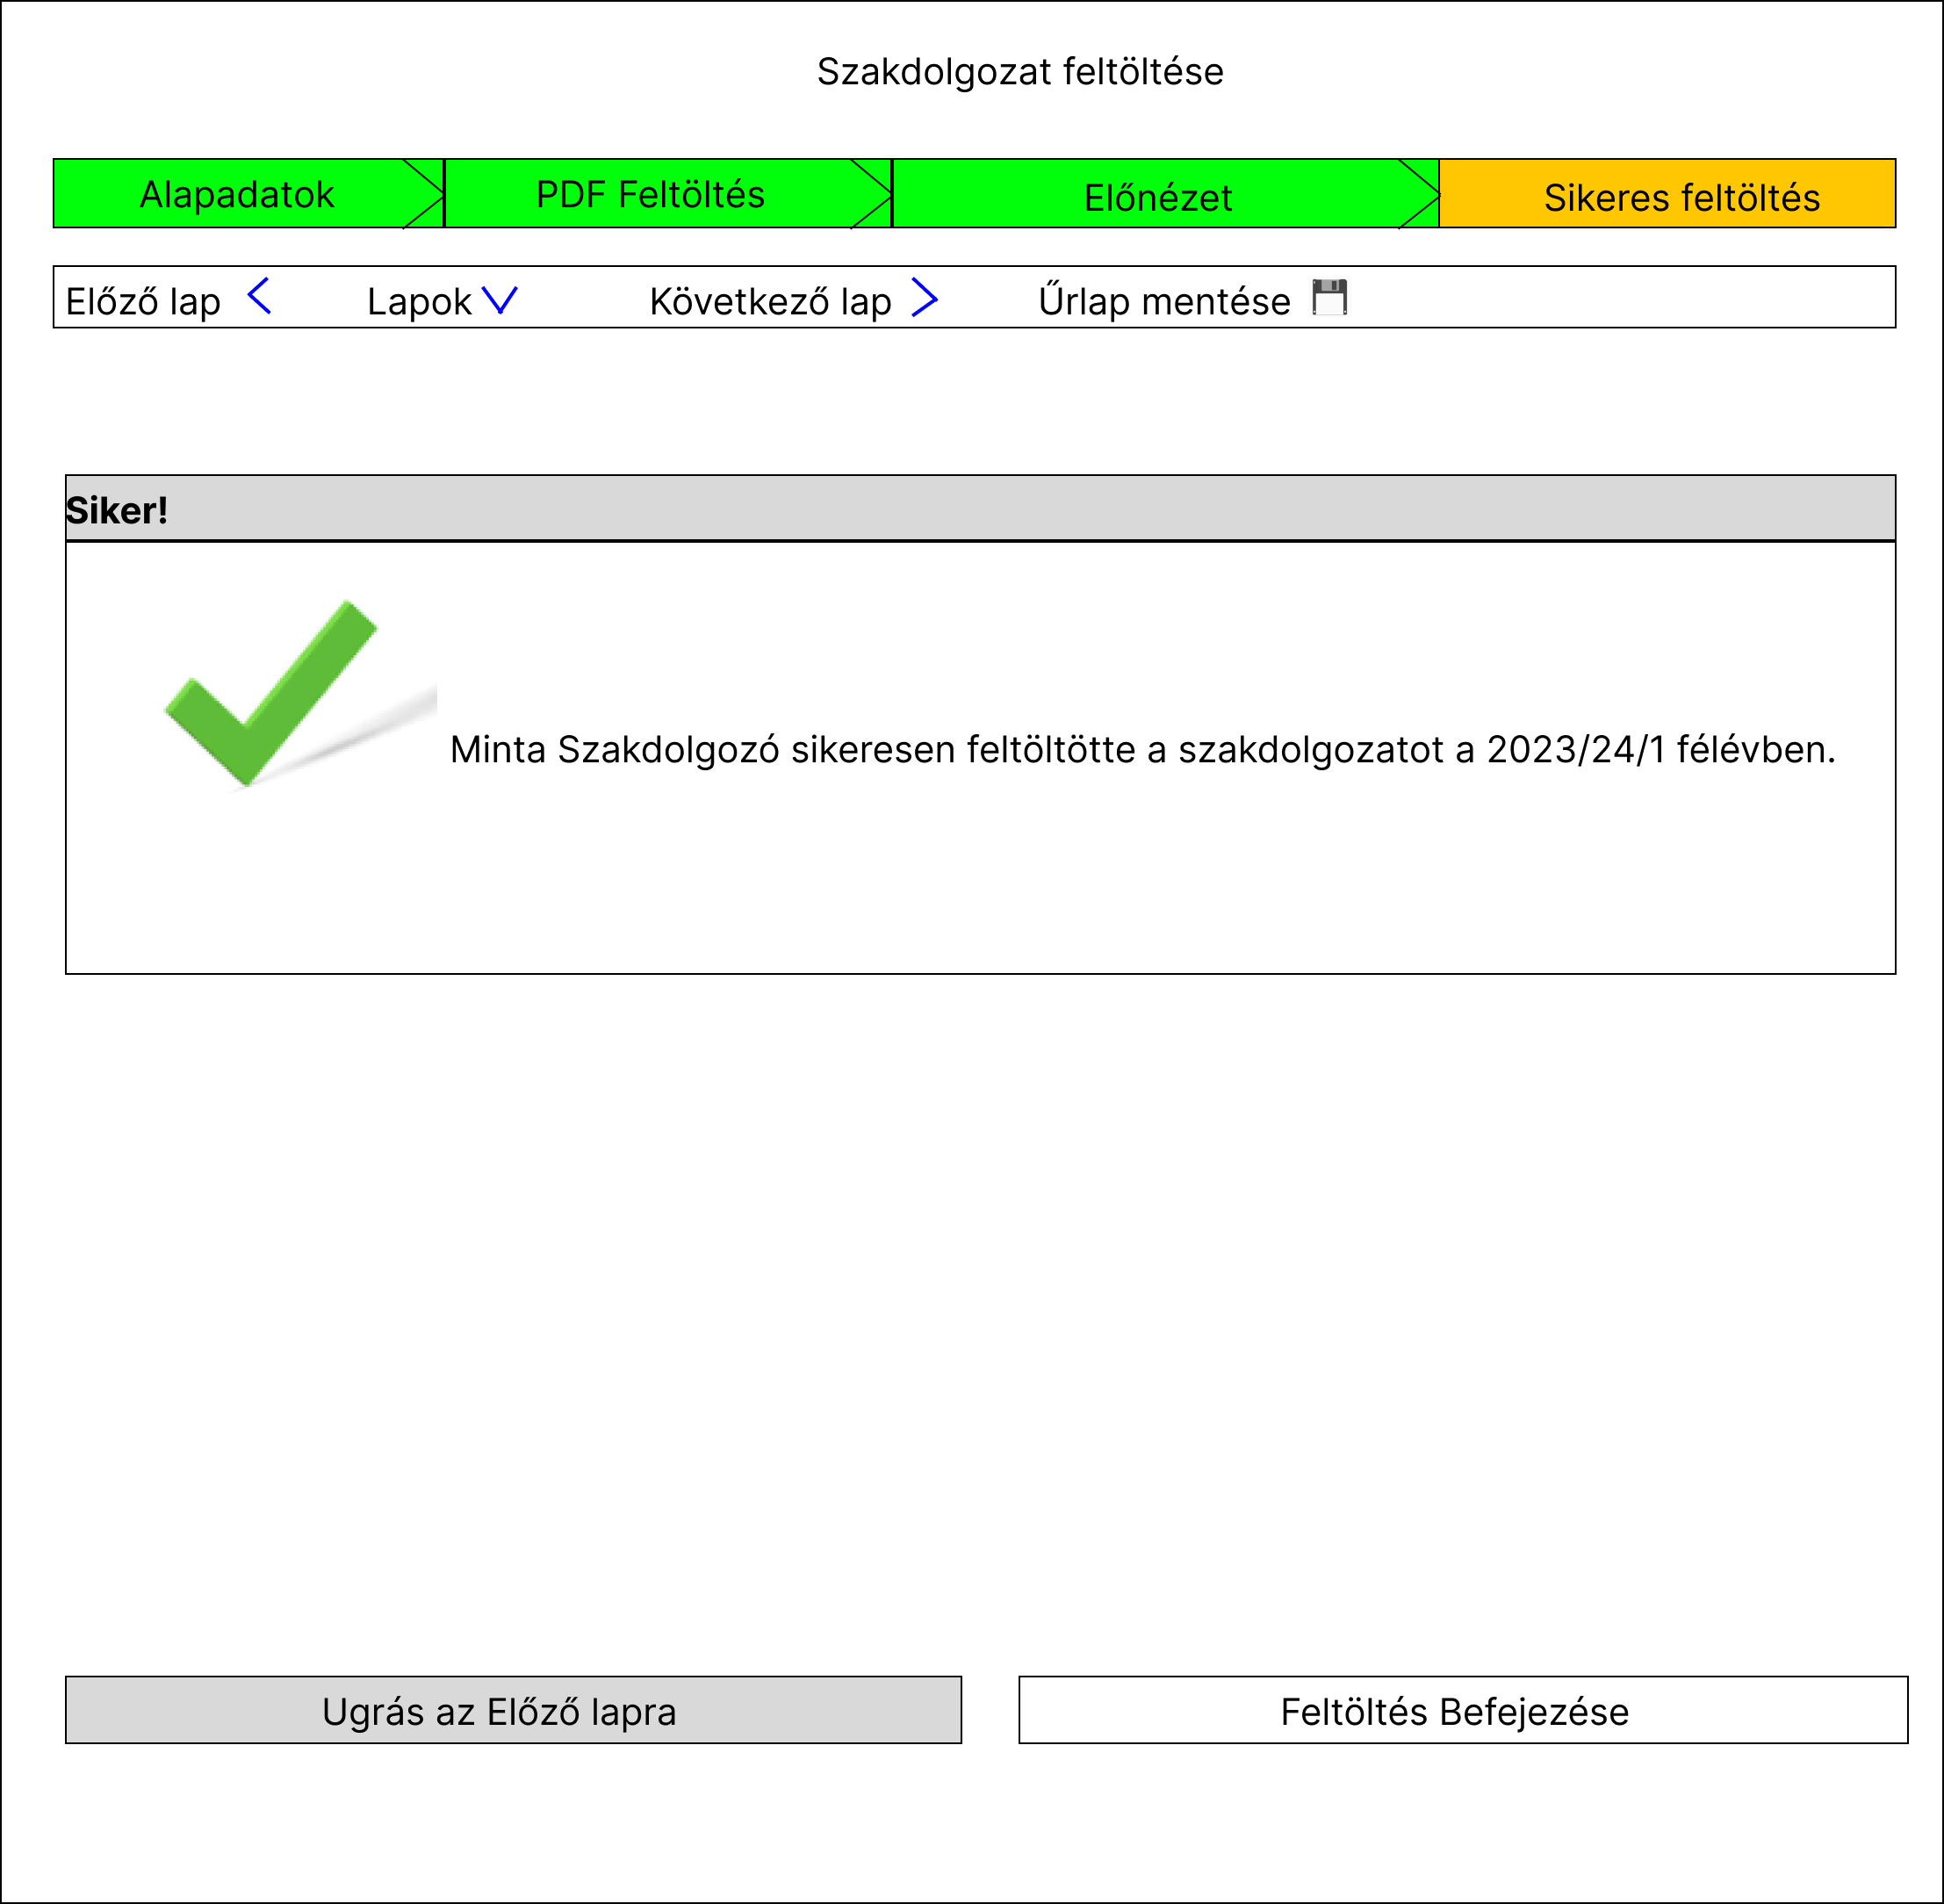
\includegraphics[width=\textwidth]{images/Web_pages/Completed.jpg}
	\caption{}
	\label{fig:Completed}
\end{figure}

Megtörtént a szakdolgozat sikeres feltöltése.

\subsection{Szakdolgozatok státusza (Thesis\_Status)}

\begin{figure}
	\centering
	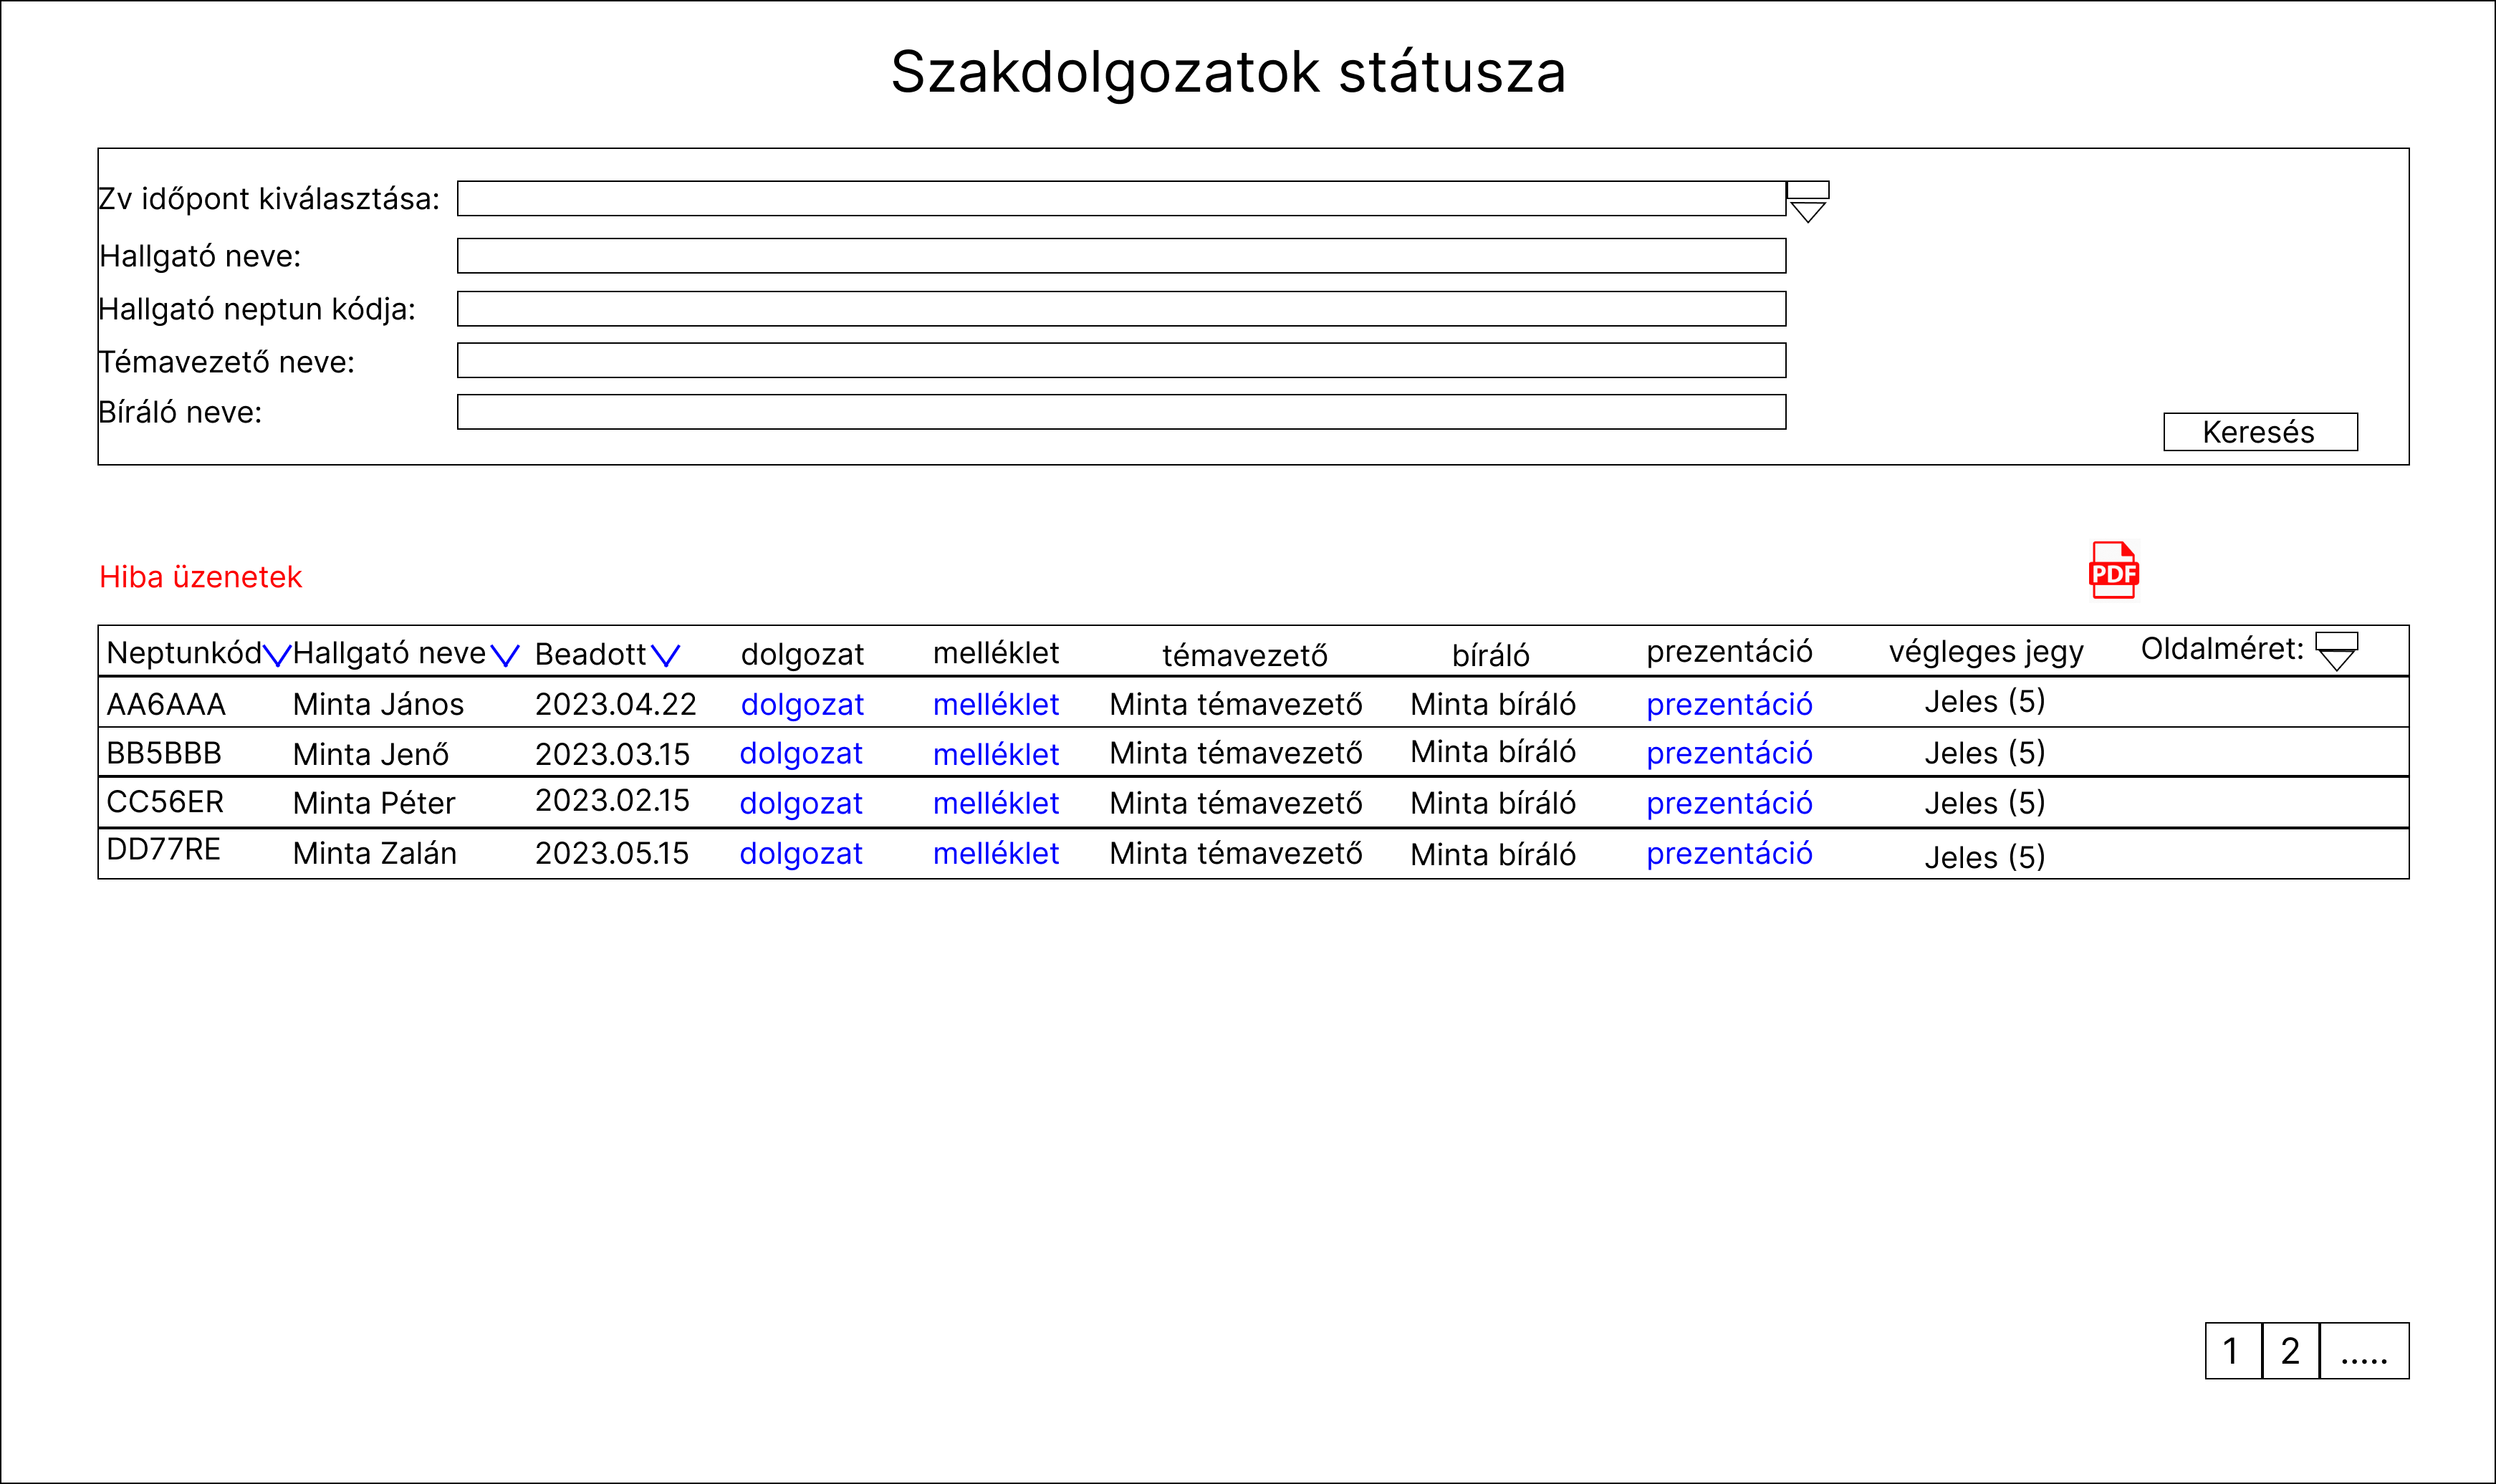
\includegraphics[width=\textwidth]{images/Web_pages/Thesis_Status.jpg}
	\caption{}
	\label{fig:Thesis_Status}
\end{figure}

A szakdolgozatok státuszáról egy összefoglaló táblázat látható.

Lehetséges hibaüzenetek:
\begin{itemize}
	\item Nem adtál meg adatot
	\item Nincs találat
\end{itemize}

\subsection{Szakdolgozat Bírálat (Thesis\_Review)}

\begin{figure}
	\centering
	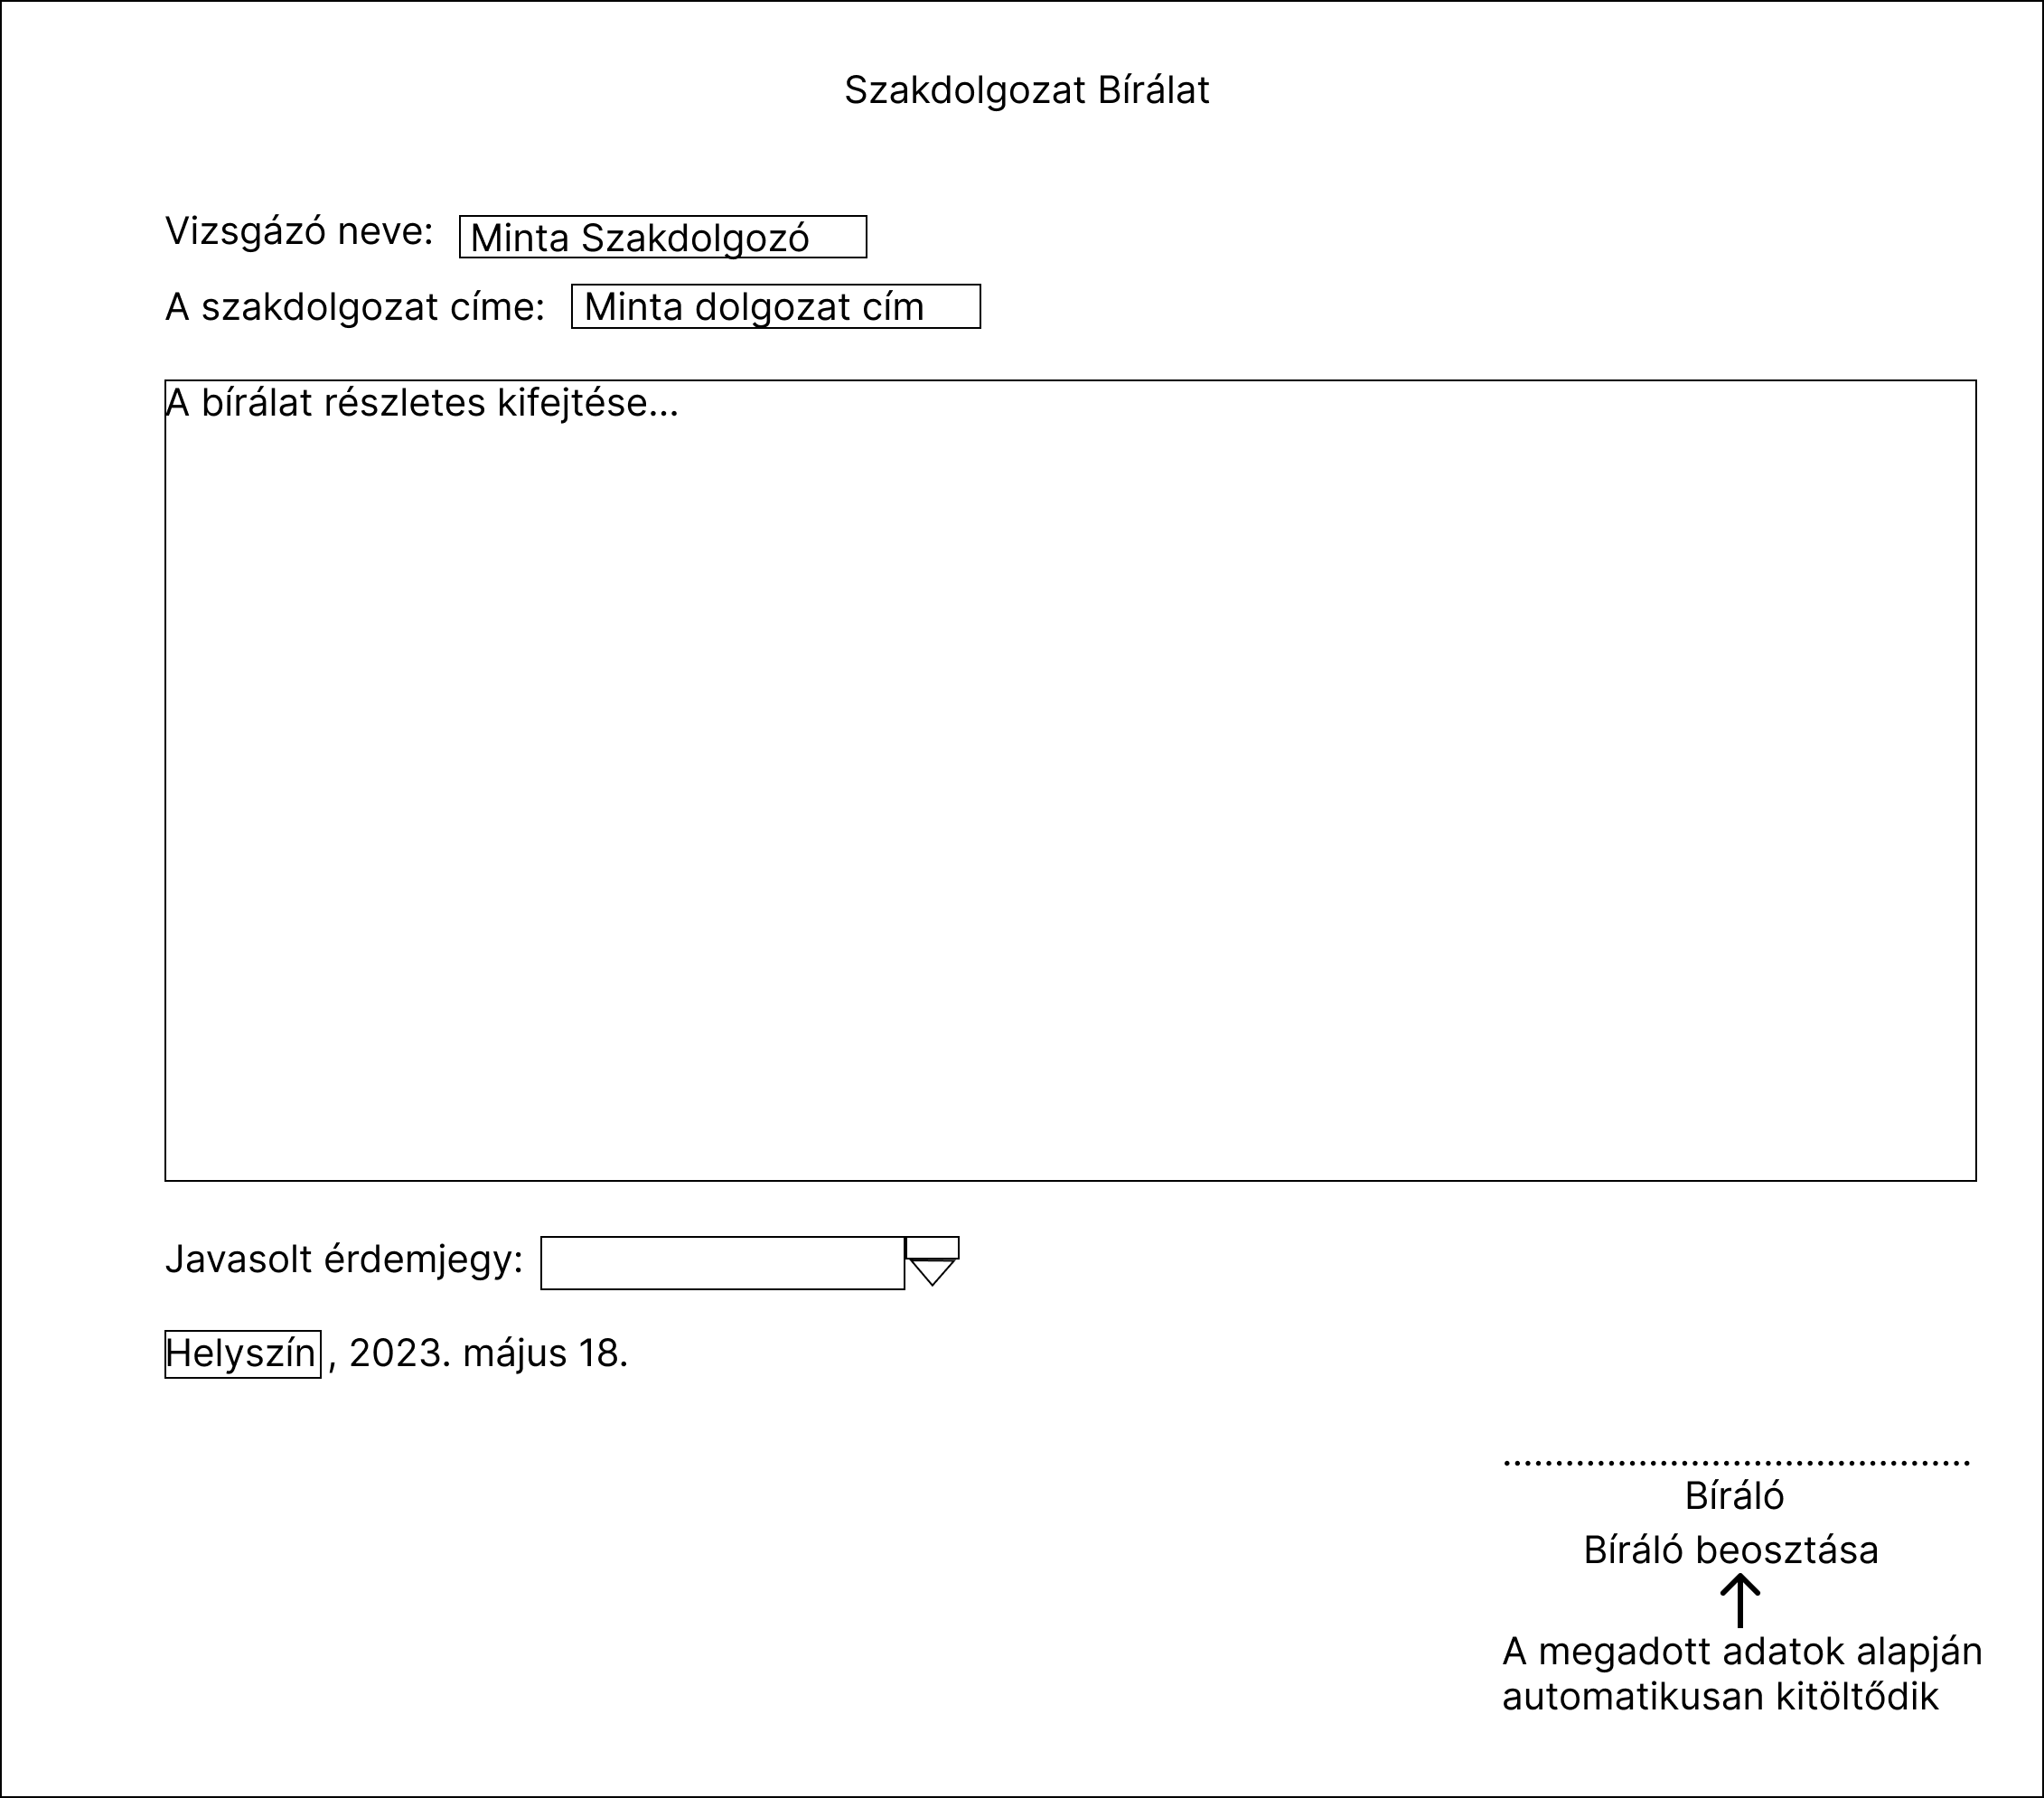
\includegraphics[width=\textwidth]{images/Web_pages/Thesis_Review.jpg}
	\caption{}
	\label{fig:Thesis_Review}
\end{figure}

A *Témavezető* és a *Bíráló* itt írhatja meg a bírálatot.

\subsection{Bírálatok státusza (Report\_Status)}

\begin{figure}
	\centering
	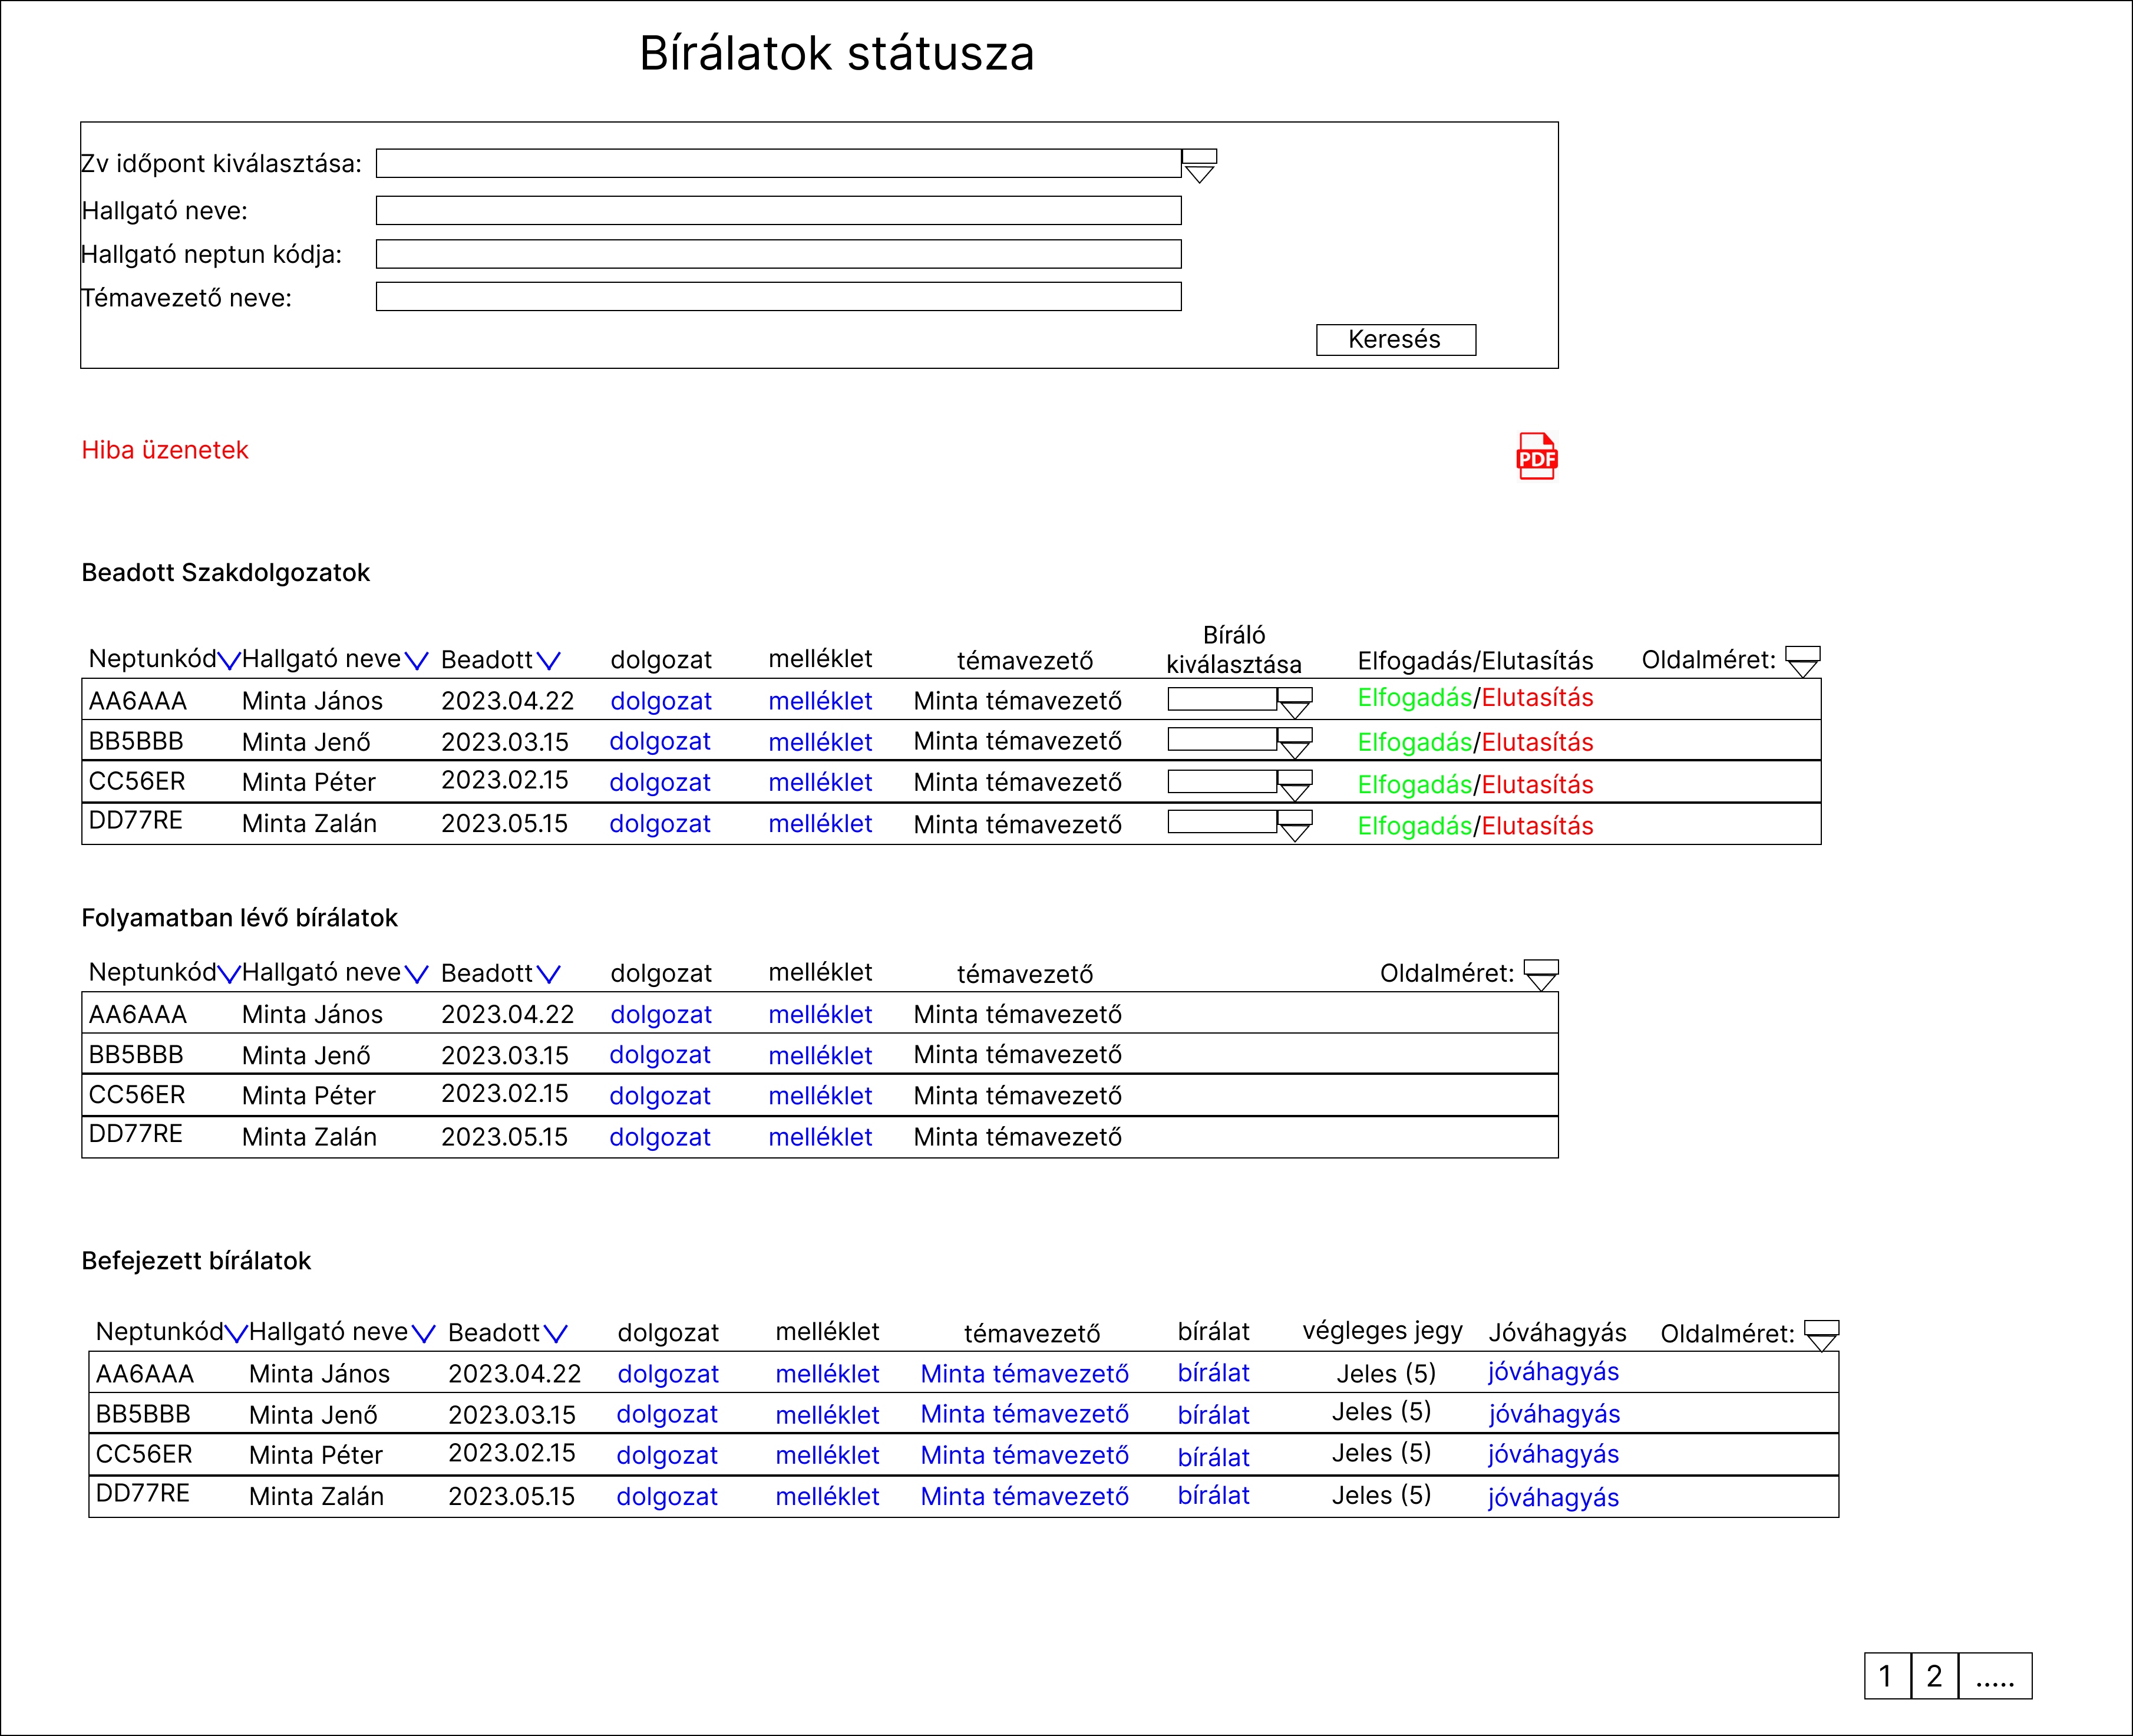
\includegraphics[width=\textwidth]{images/Web_pages/Report_Status.jpg}
	\caption{}
	\label{fig:Report_Status}
\end{figure}

\subsection{Záróvizsga létrehozása (ZV\_Create)}

\begin{figure}
	\centering
	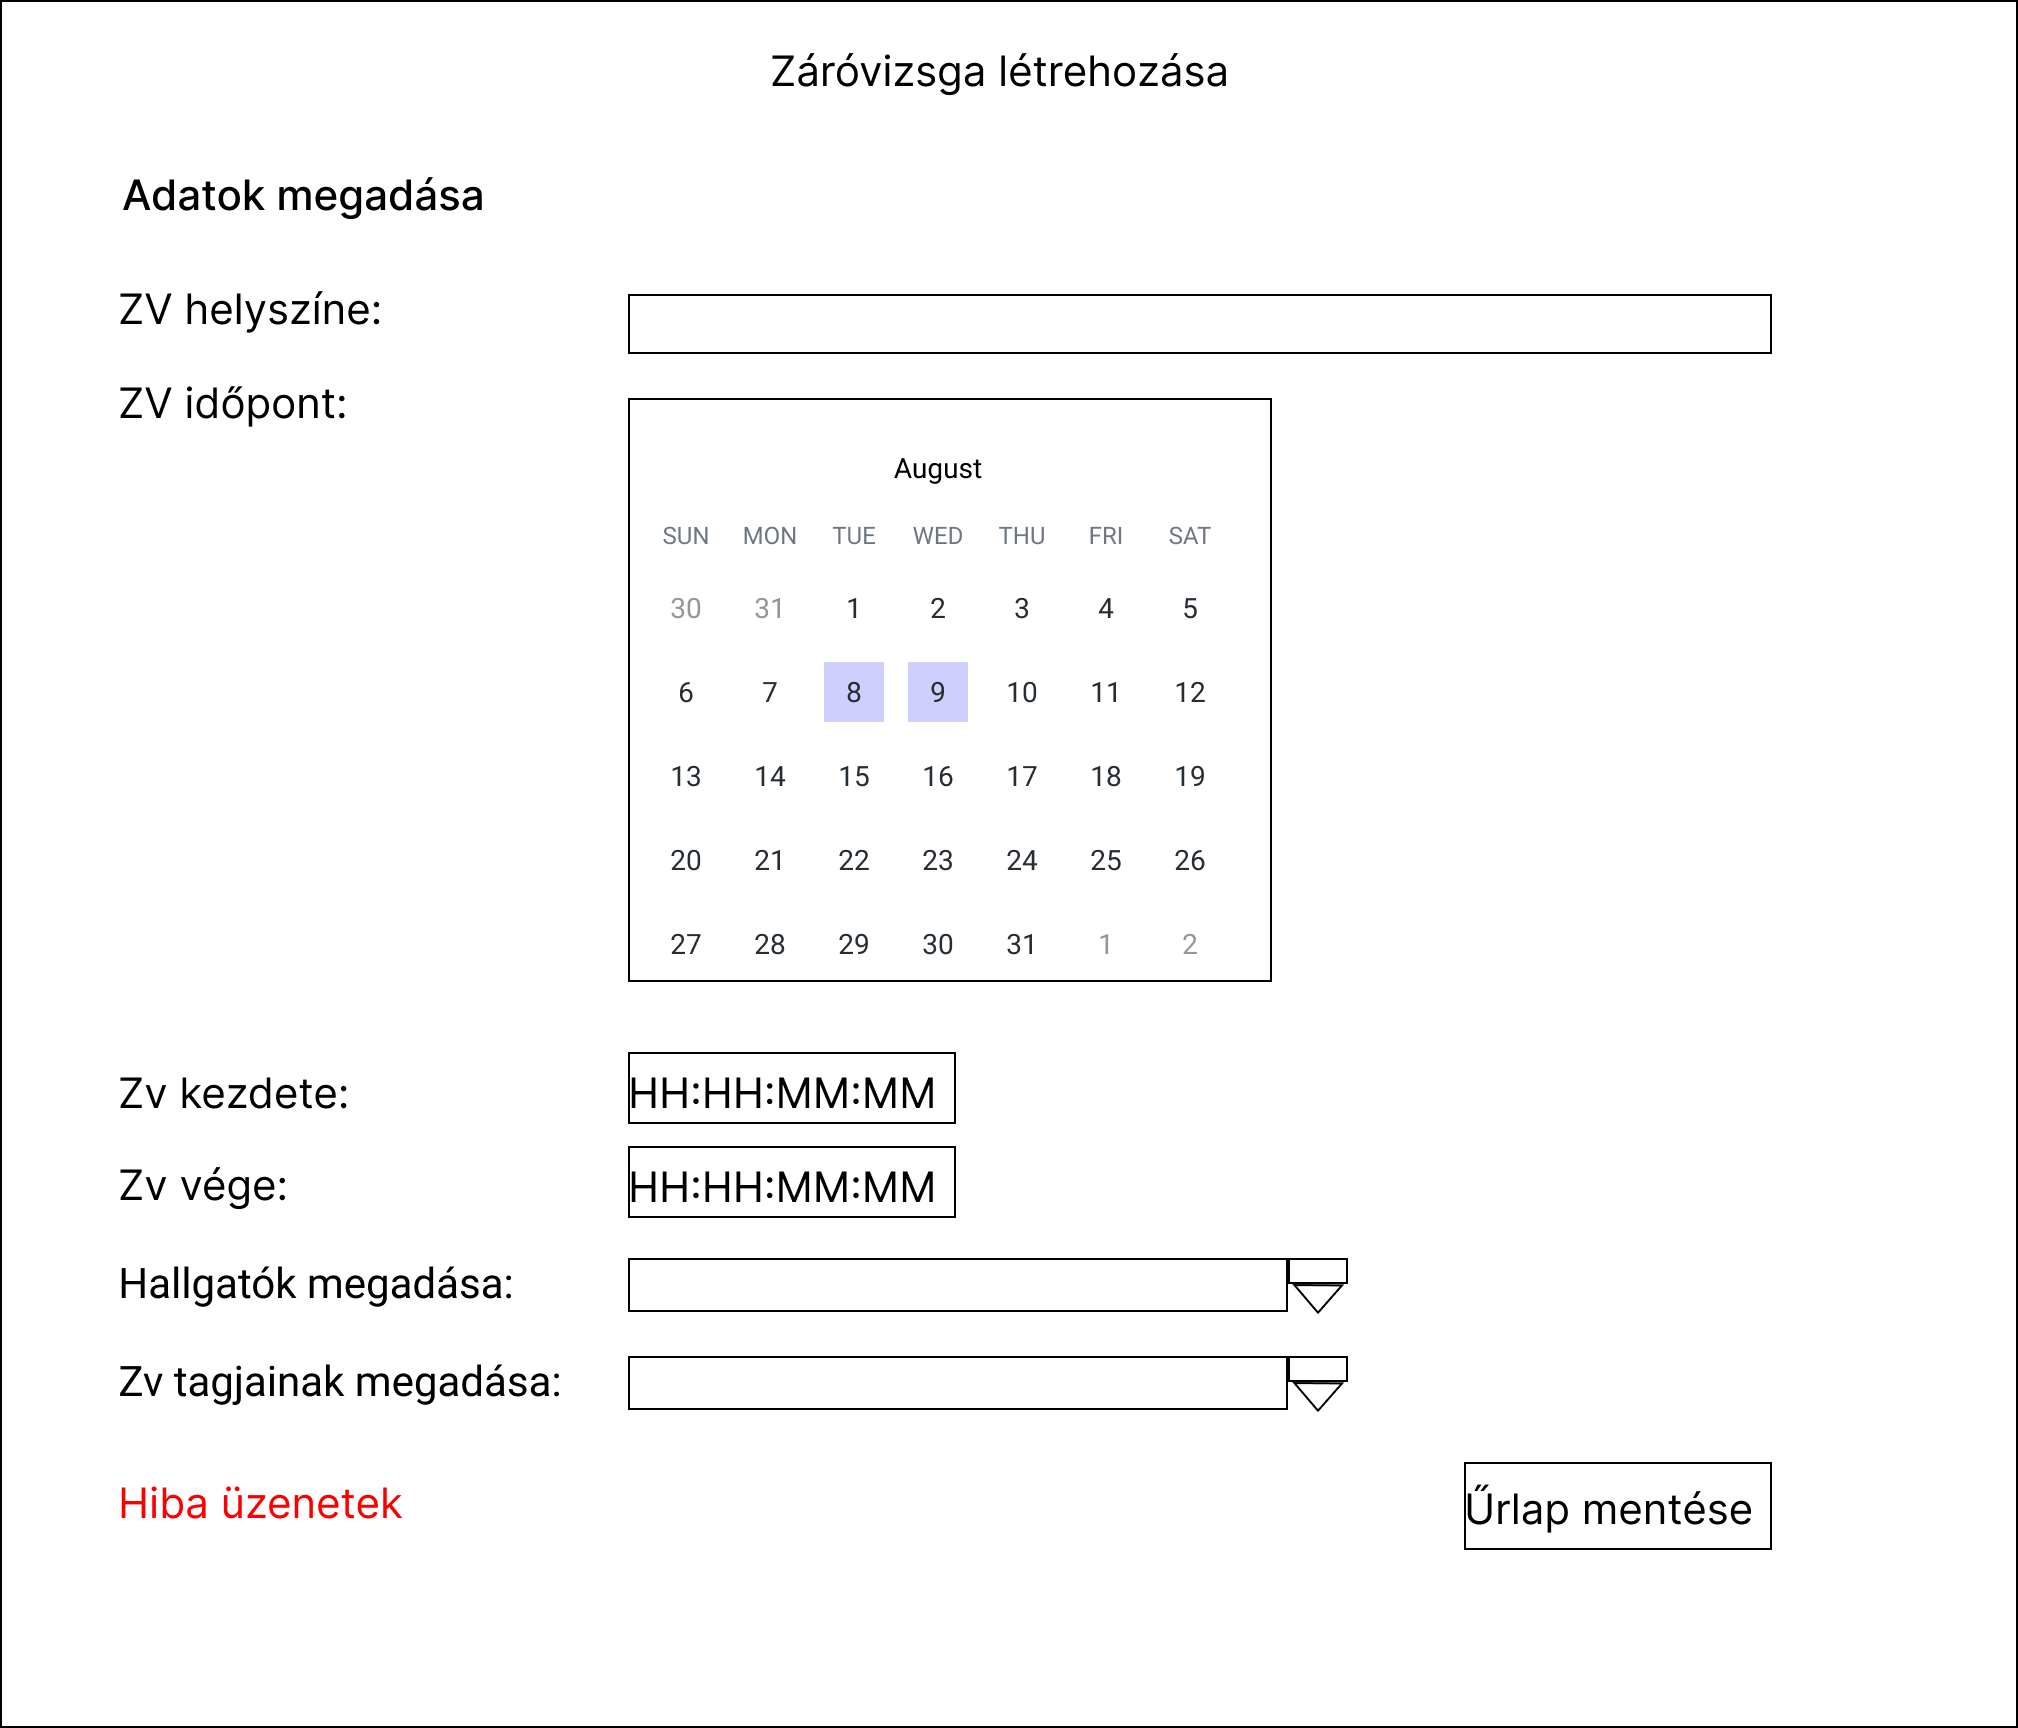
\includegraphics[width=\textwidth]{images/Web_pages/ZV_Create.jpg}
	\caption{}
	\label{fig:ZV_Create}
\end{figure}

Az *Elnök* itt hozhatja létre a záróvizsgát.

\subsection{Záróvizsga jegyzőkönyv szerkesztése}

%(ZV_Report1,ZV_Report2,ZV_Report3,ZV_Report4)

Első lap

\begin{figure}
	\centering
	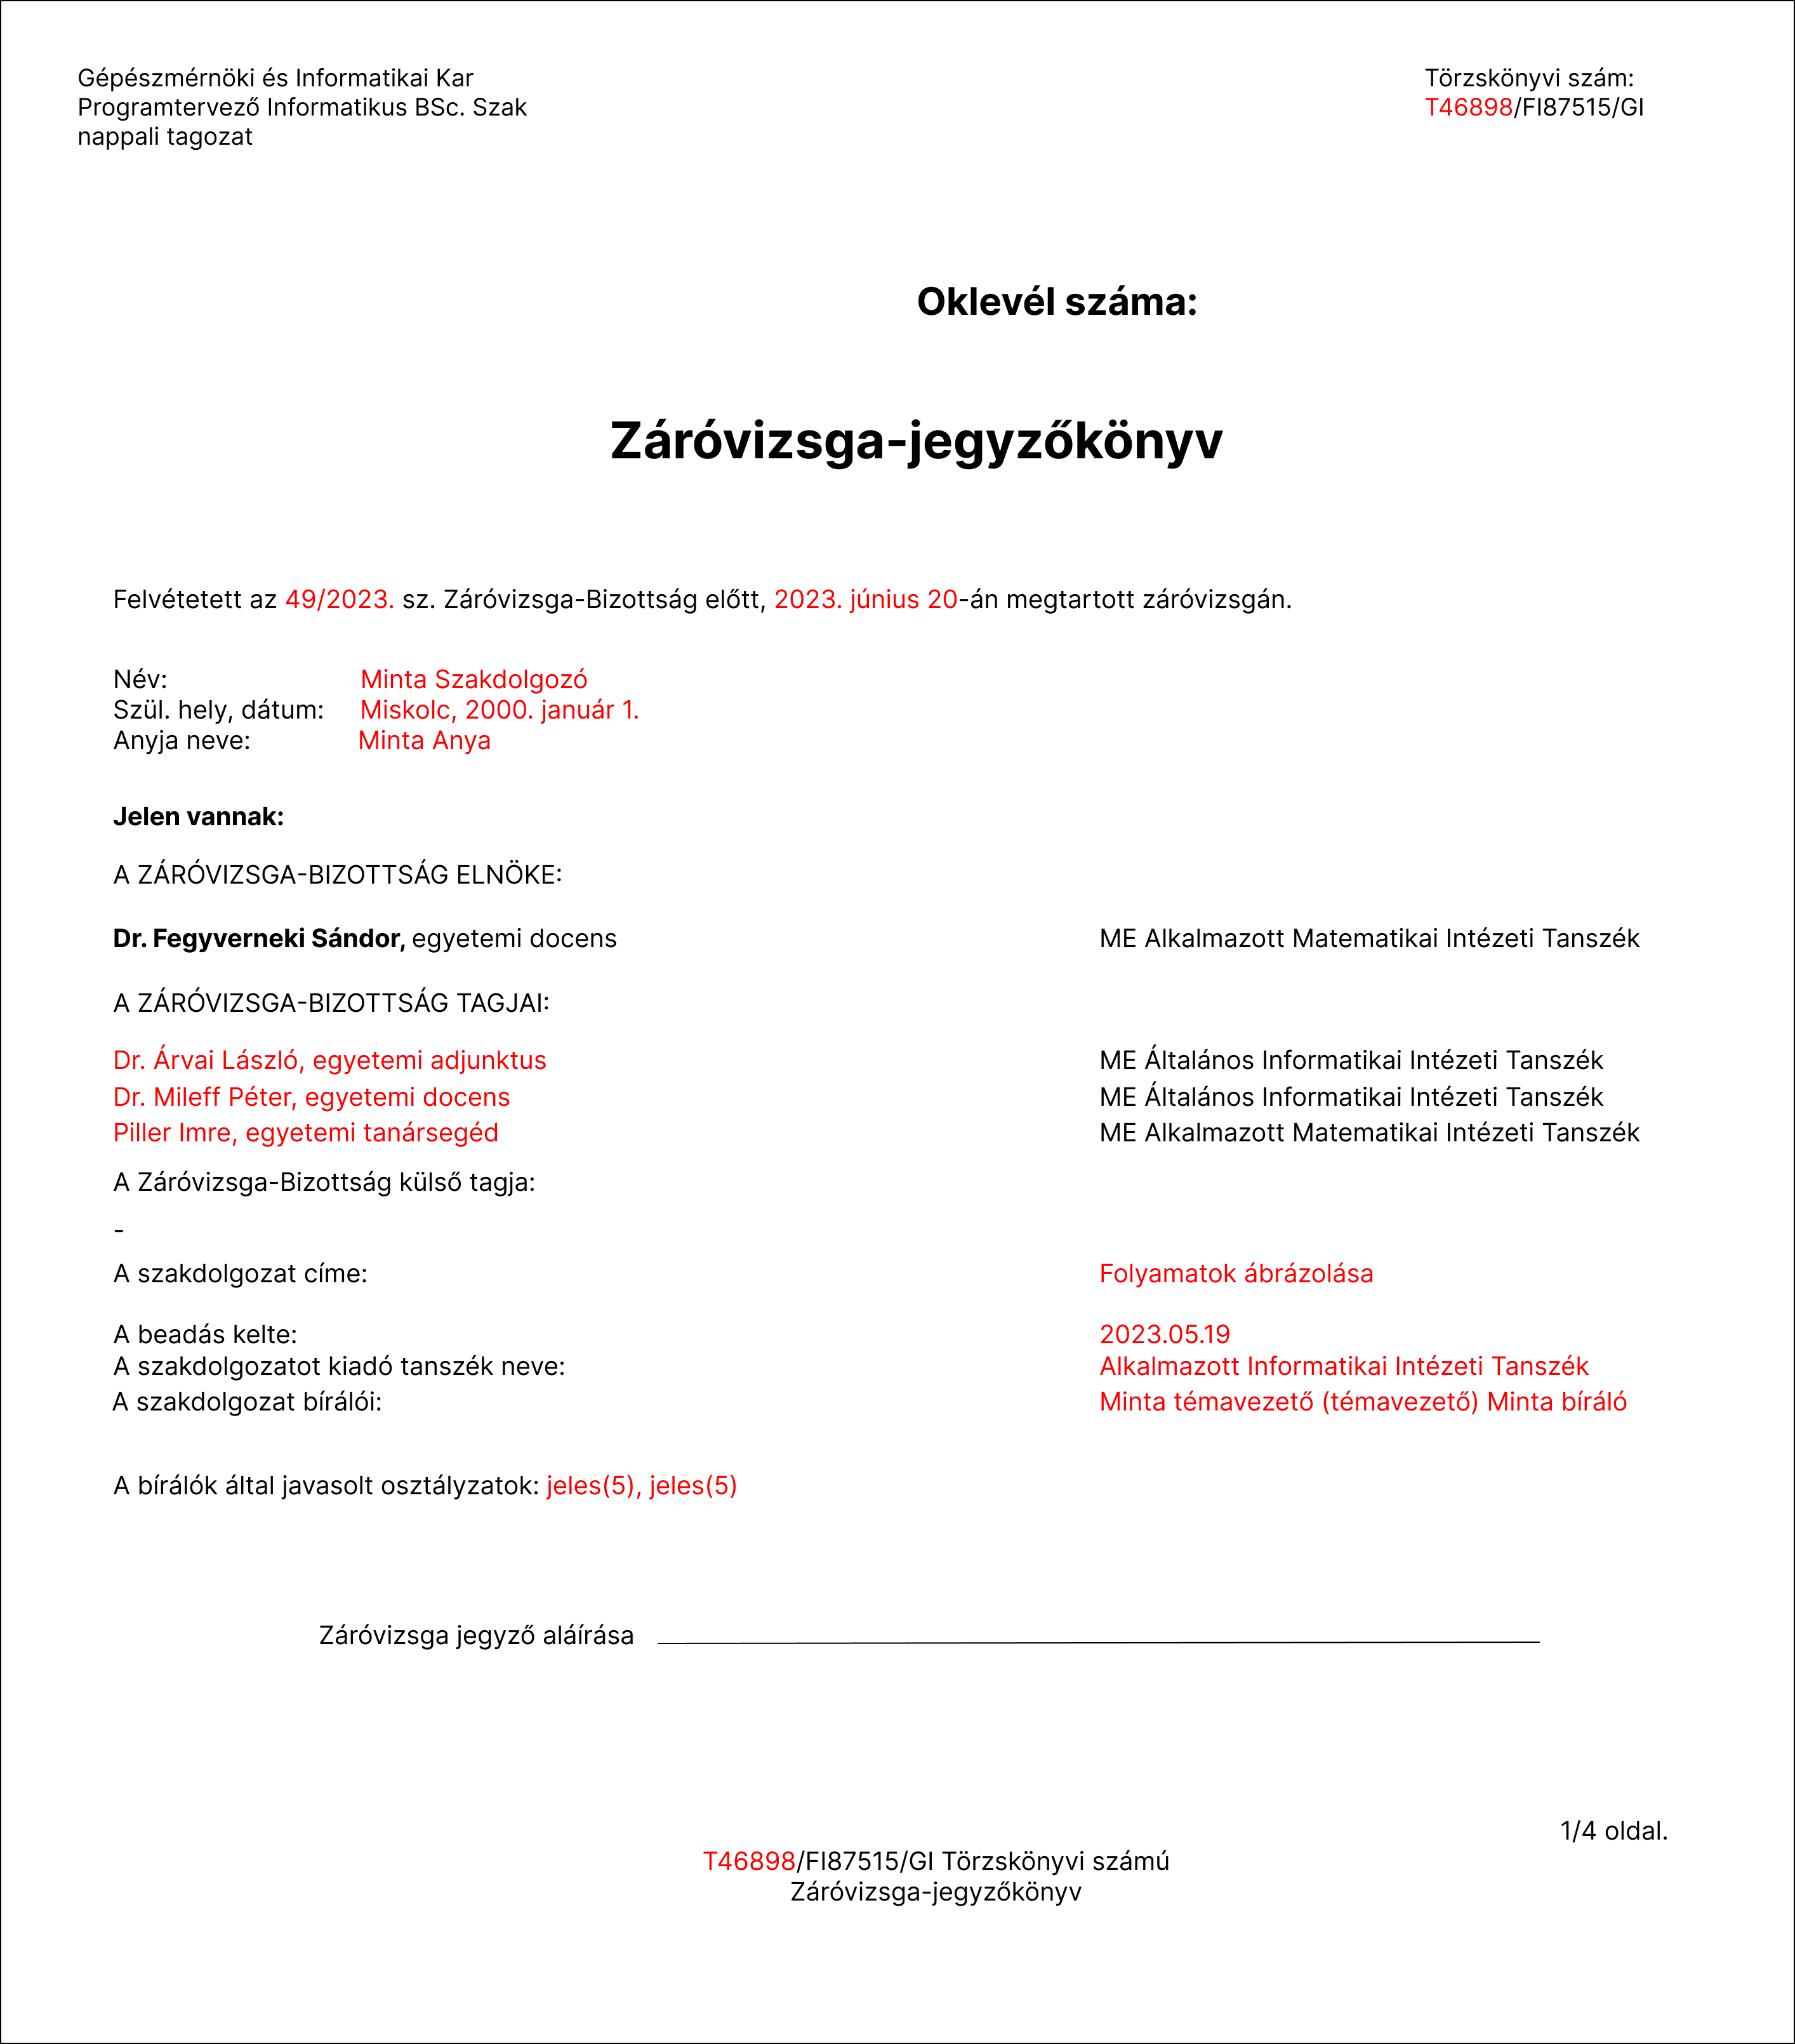
\includegraphics[width=\textwidth]{images/Web_pages/Zv_Report1.png}
	\caption{}
	\label{fig:Zv_Report1}
\end{figure}

Második lap

\begin{figure}
	\centering
	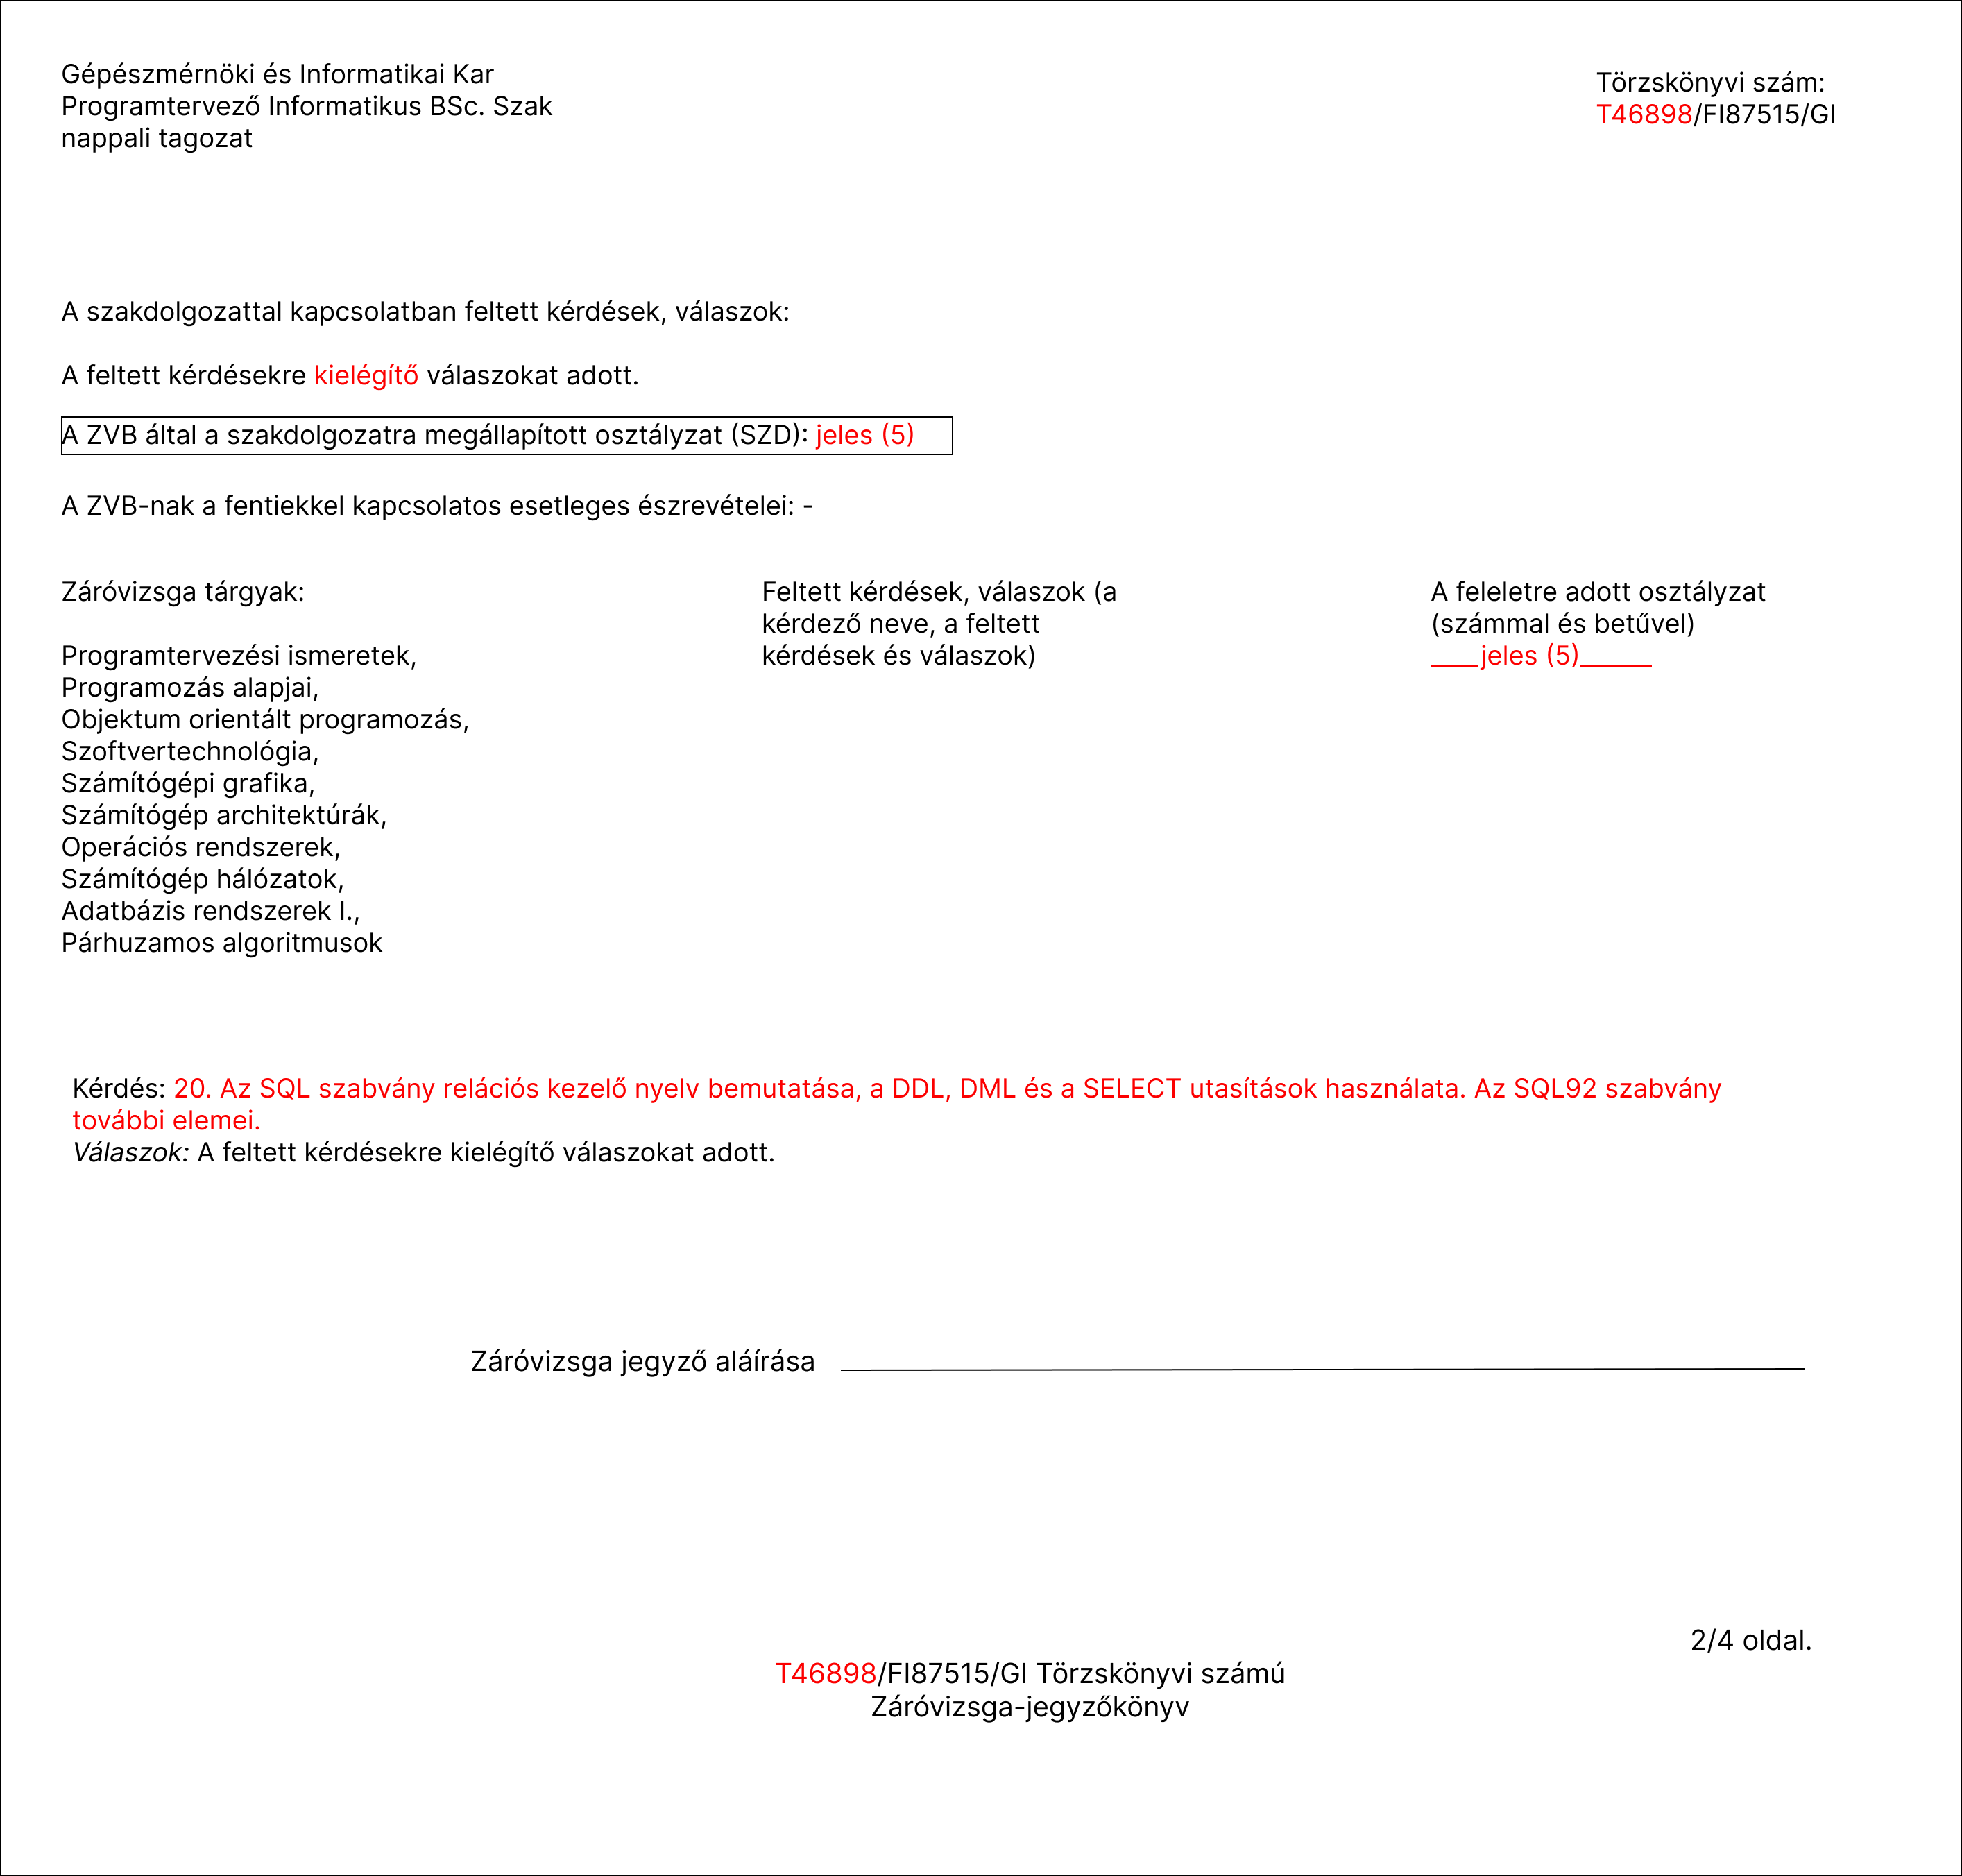
\includegraphics[width=\textwidth]{images/Web_pages/Zv_Report2.png}
	\caption{}
	\label{fig:Zv_Report2}
\end{figure}

Harmadik lap

\begin{figure}
	\centering
	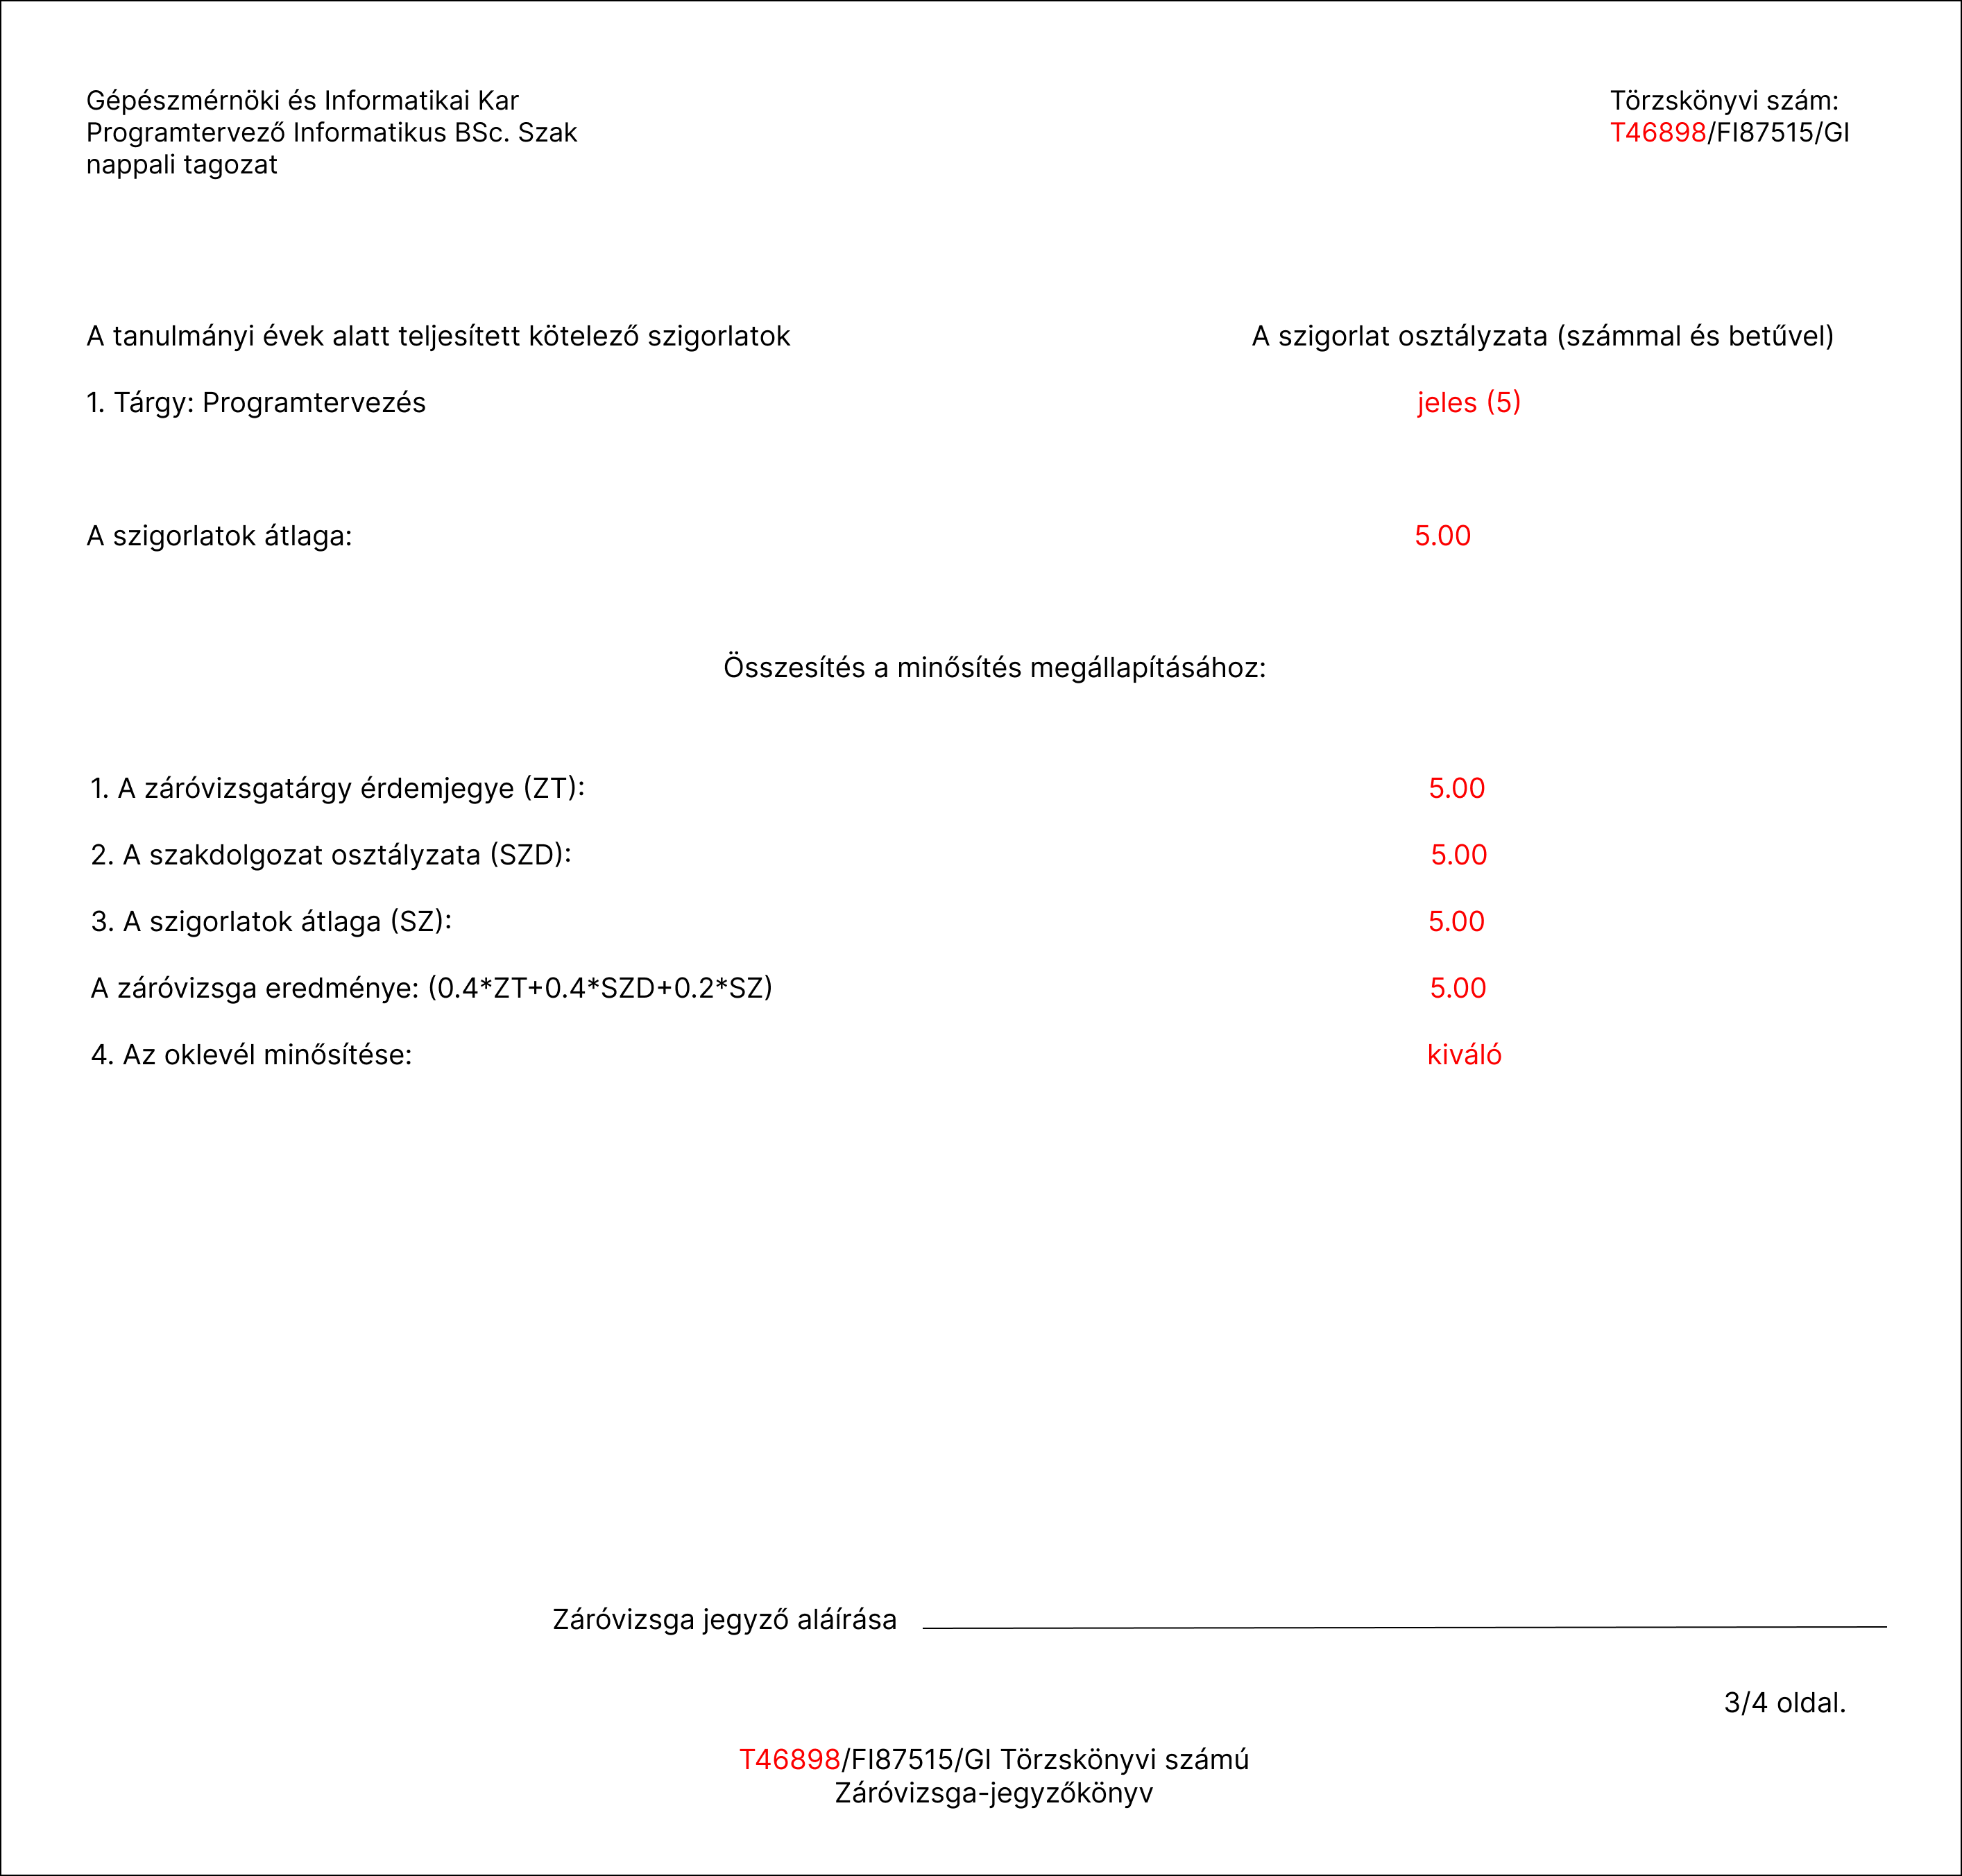
\includegraphics[width=\textwidth]{images/Web_pages/Zv_Report3.png}
	\caption{}
	\label{fig:Zv_Report3}
\end{figure}

Negyedik lap

\begin{figure}
	\centering
	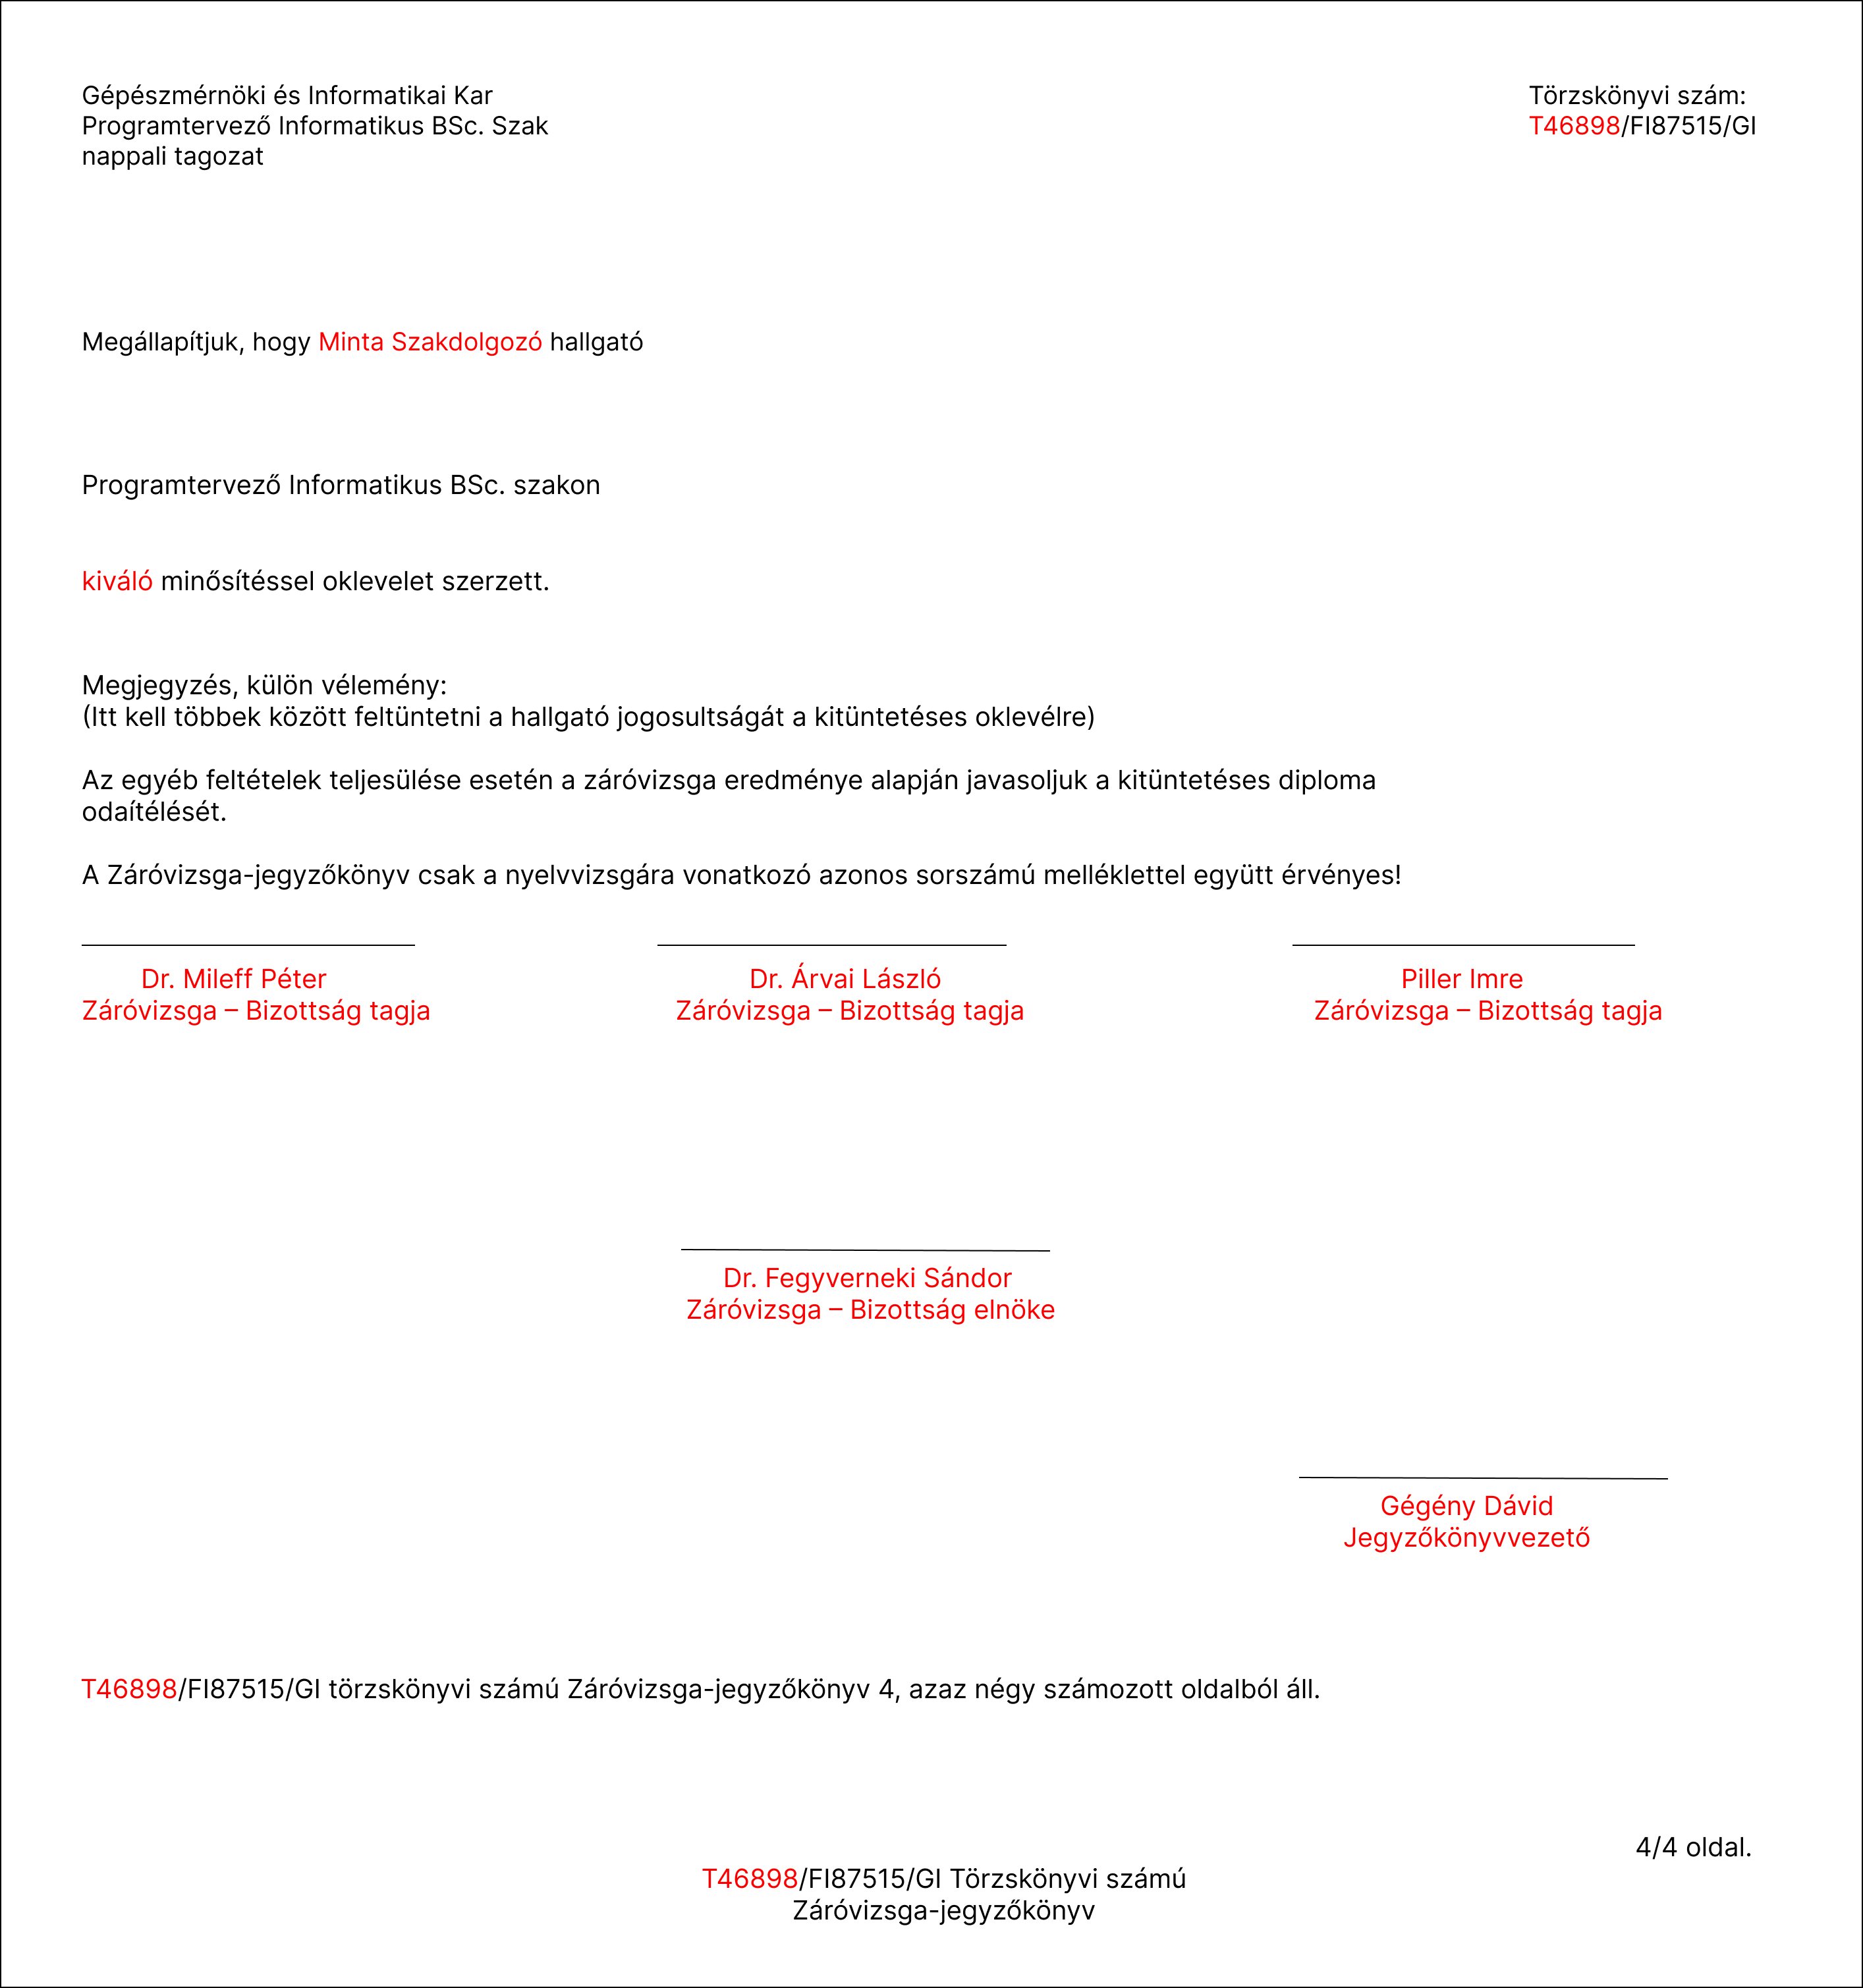
\includegraphics[width=\textwidth]{images/Web_pages/Zv_Report4.png}
	\caption{}
	\label{fig:Zv_Report4}
\end{figure}

A záróvizsga jegyzőkönyv szerkesztése látható itt. Pirossal azok a részek vannak kiemelve, amelyeket módosítani lehet.

\subsection{Záróvizsga jegyek rögzítése és Záróvizsga jegyzőkönyv letöltése}

%(ZV_Status)

\begin{figure}
	\centering
	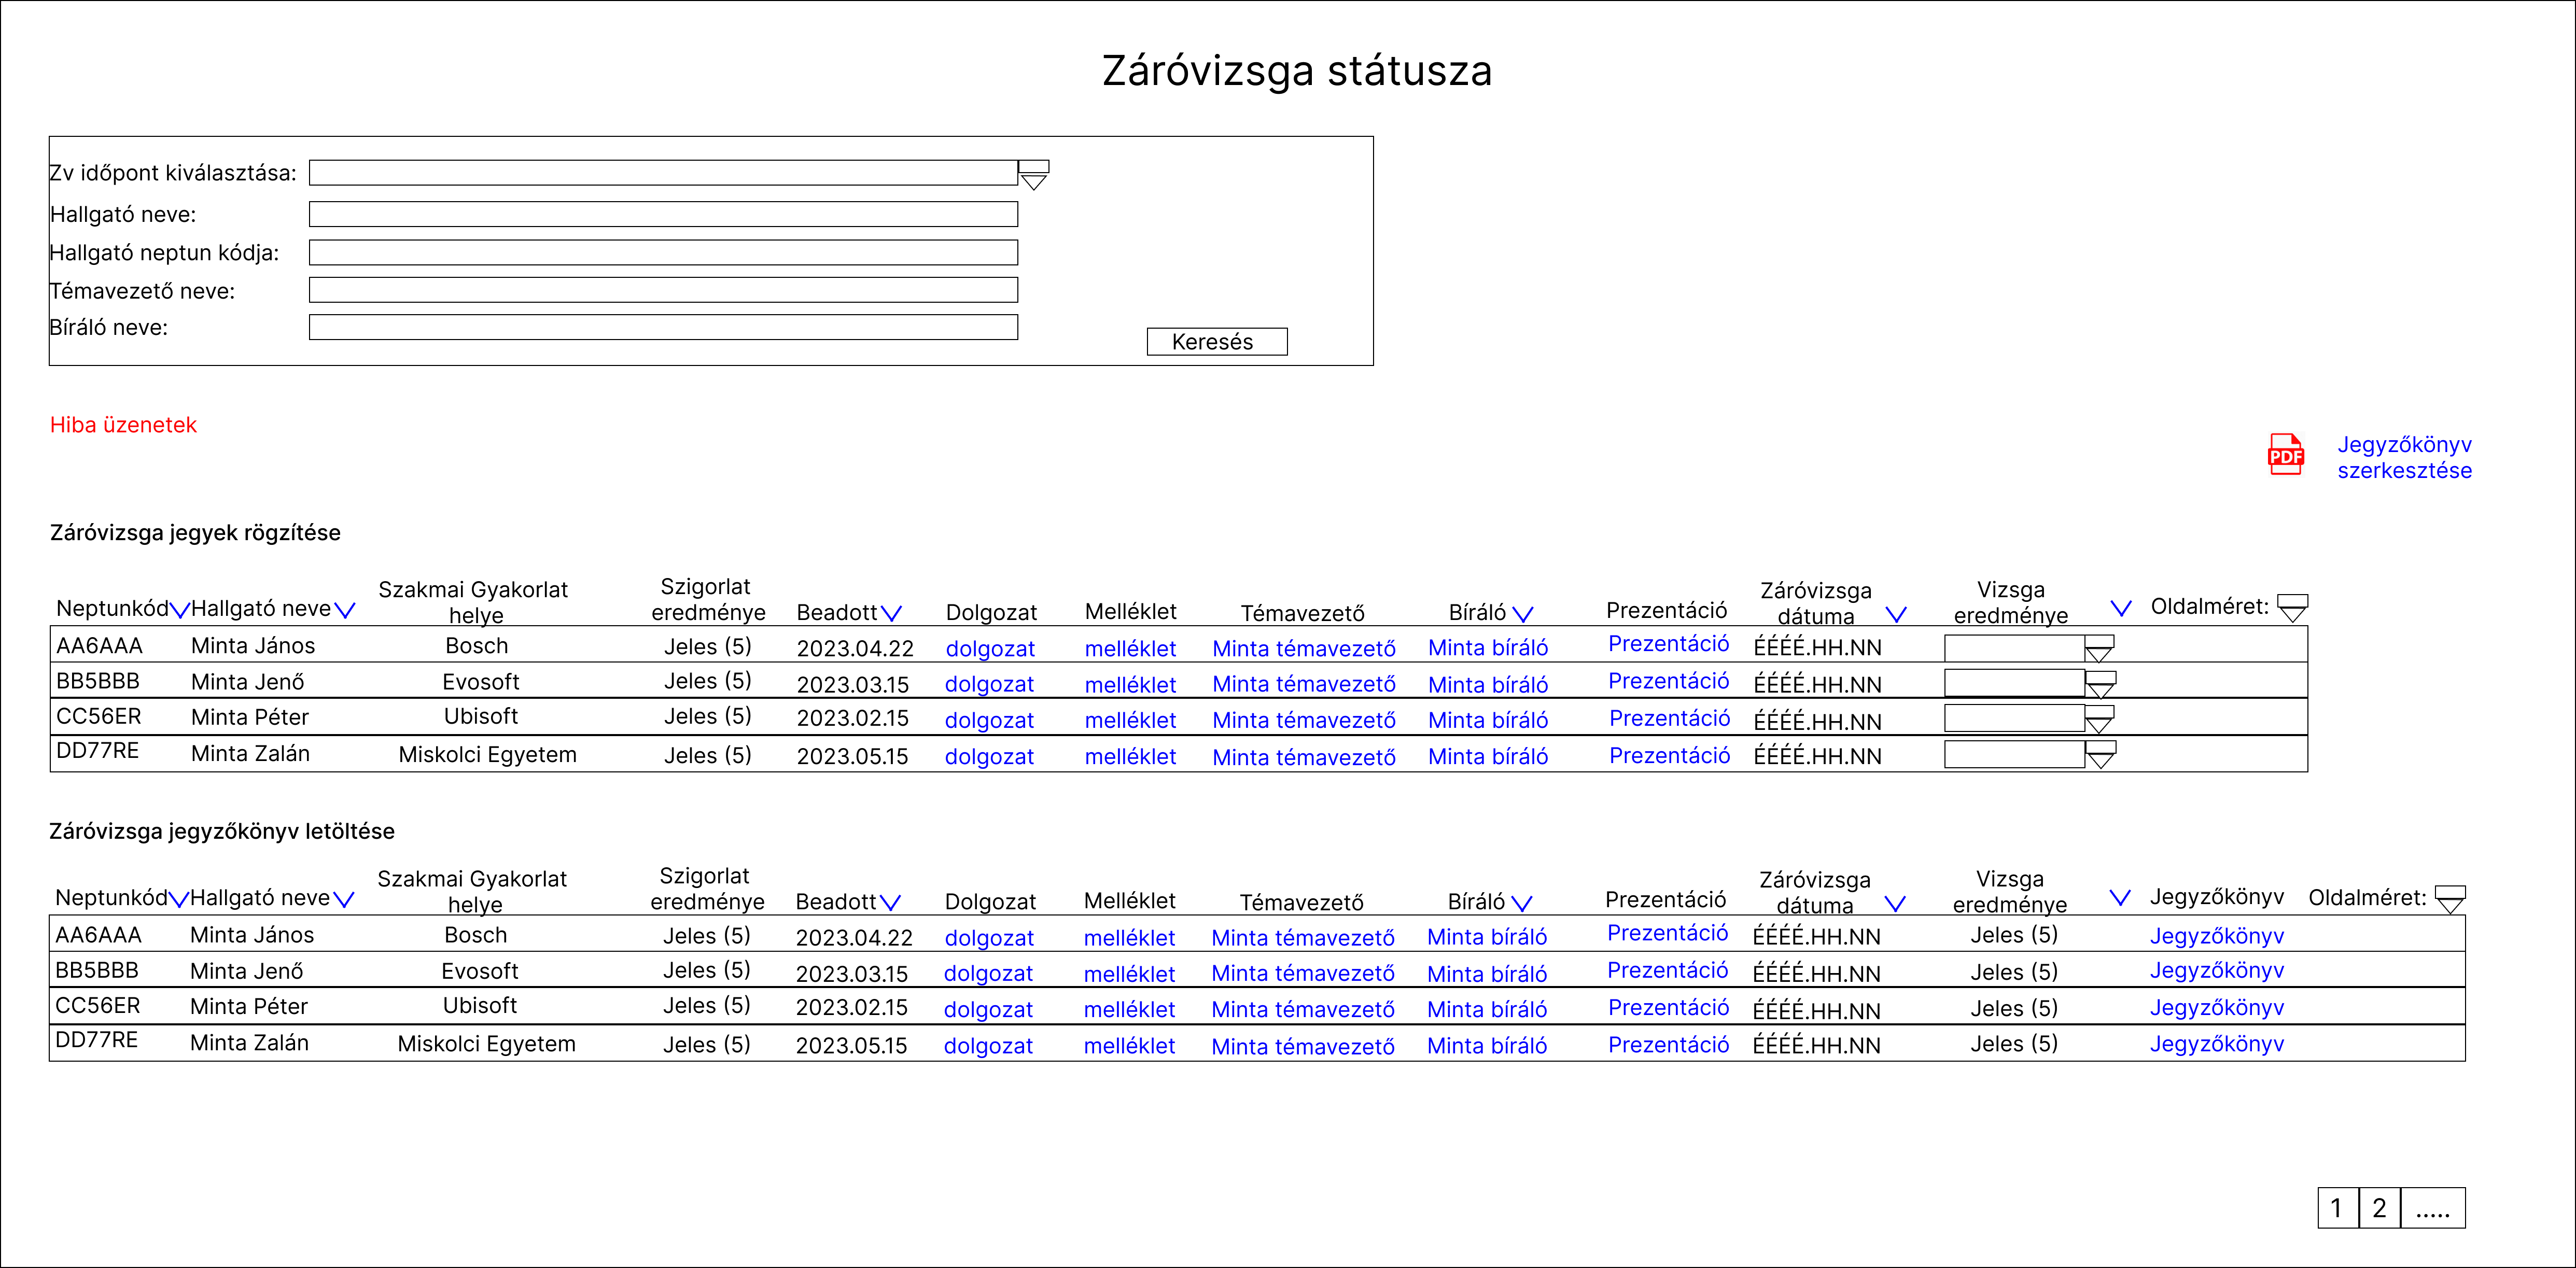
\includegraphics[width=\textwidth]{images/Web_pages/Zv_Status.png}
	\caption{}
	\label{fig:Zv_Status}
\end{figure}

\begin{itemize}
	\item A *Jegyző* az *Elnök* és a *Témavezető* itt rögzítheti a Záróvizsgán kapott érdemjegyeket.
	\item A felhasználók innen tölthetik le a jegyzőkönyvet.
\end{itemize}

\subsection{Saját profil [Hallgató] (My\_Profile\_Student)}

\begin{figure}
	\centering
	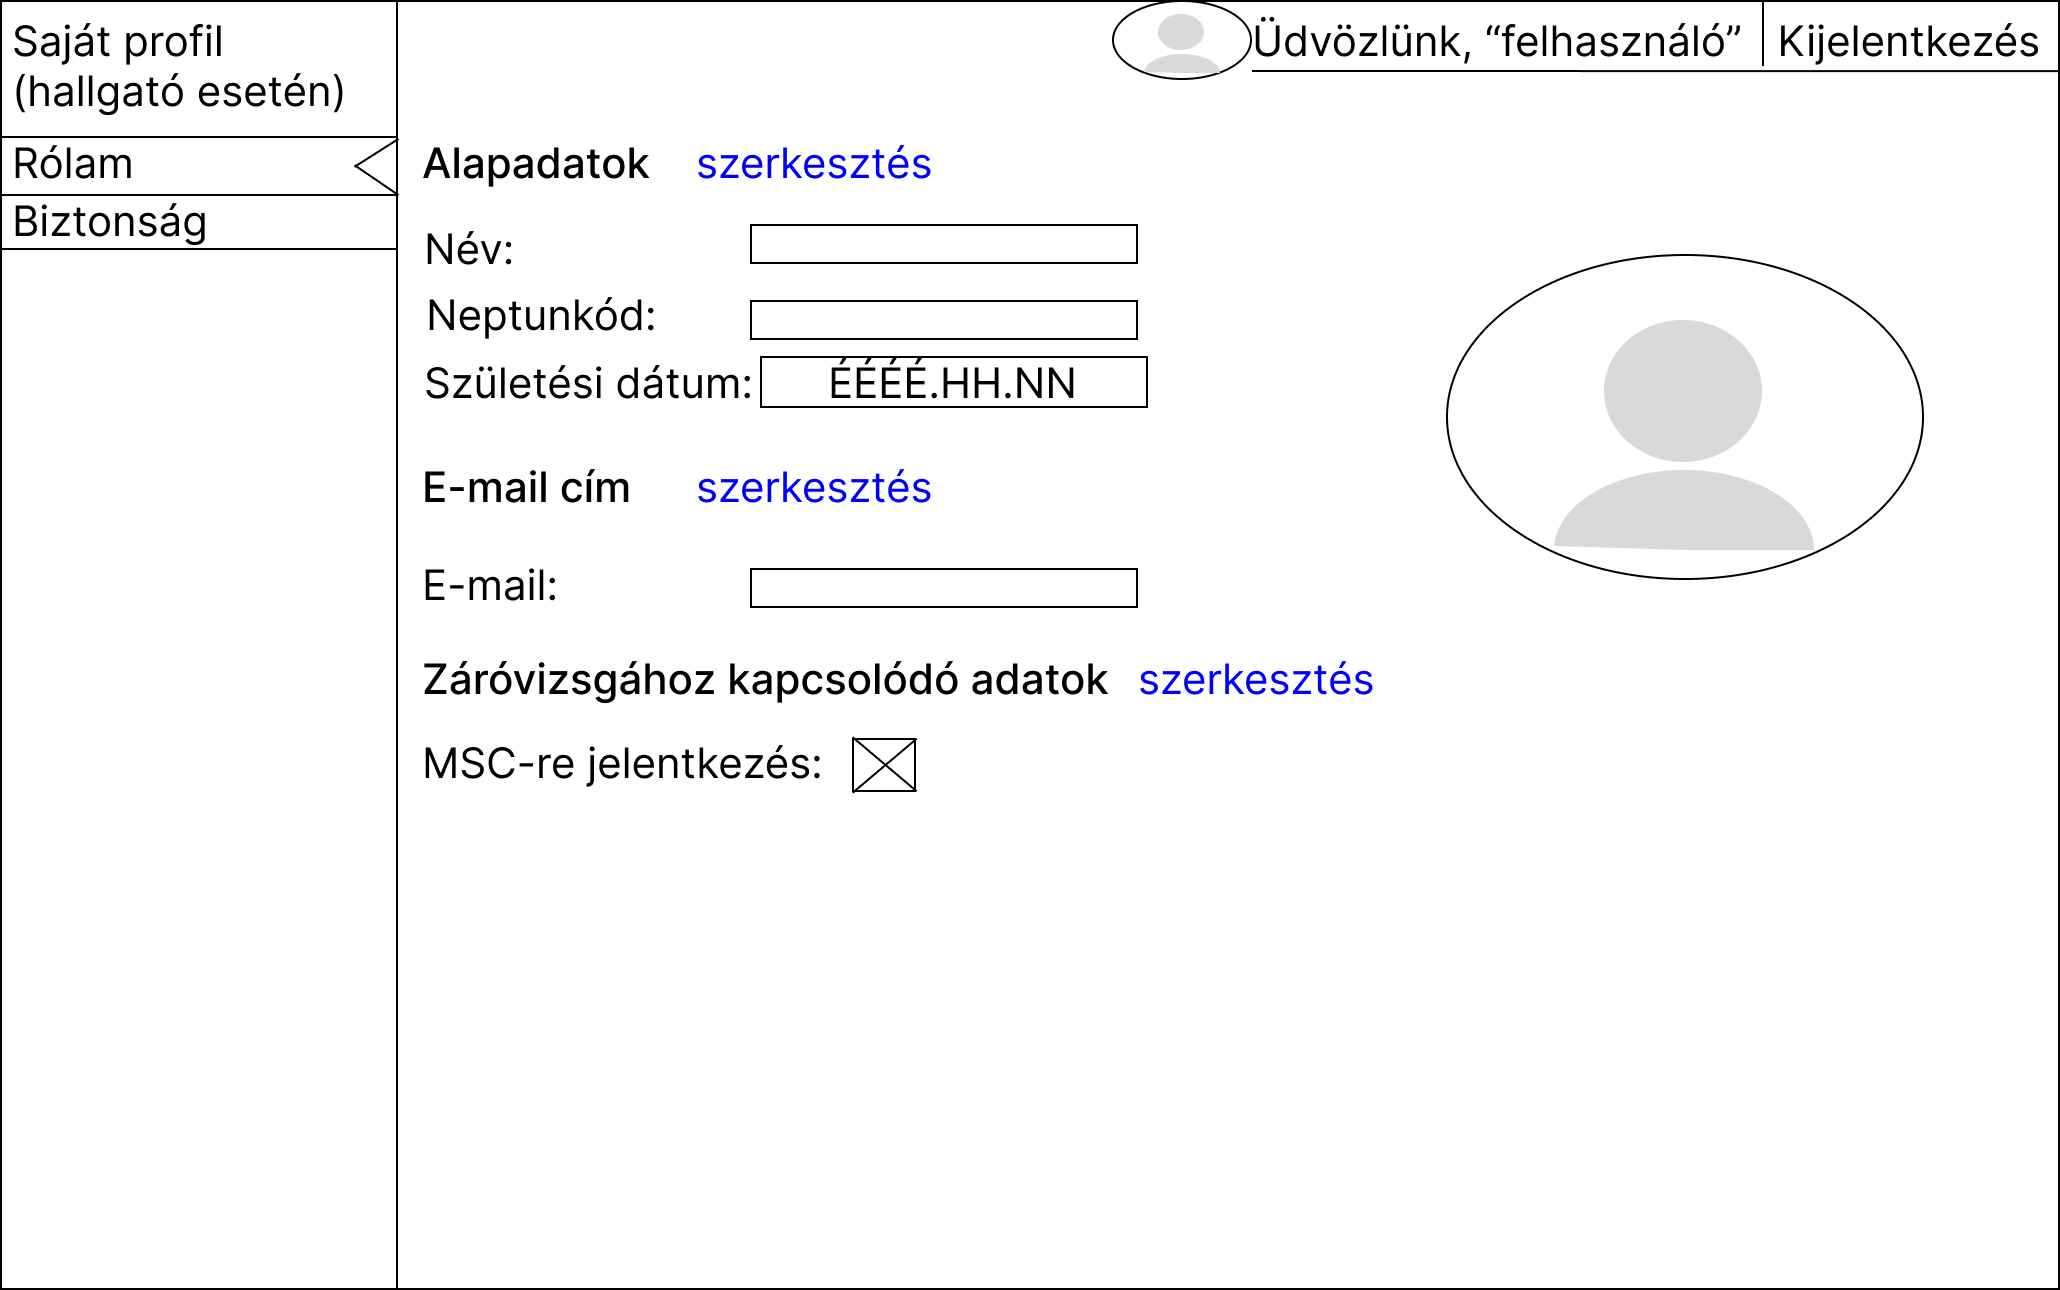
\includegraphics[width=\textwidth]{images/Web_pages/My_Profile_Student.jpg}
	\caption{}
	\label{fig:My_Profile_Student}
\end{figure}

A Hallgató saját profilja látható a megadott adatok alapján.

\subsection{Saját profil [A többi szerepkörre] (My\_Profile)}

\begin{figure}
	\centering
	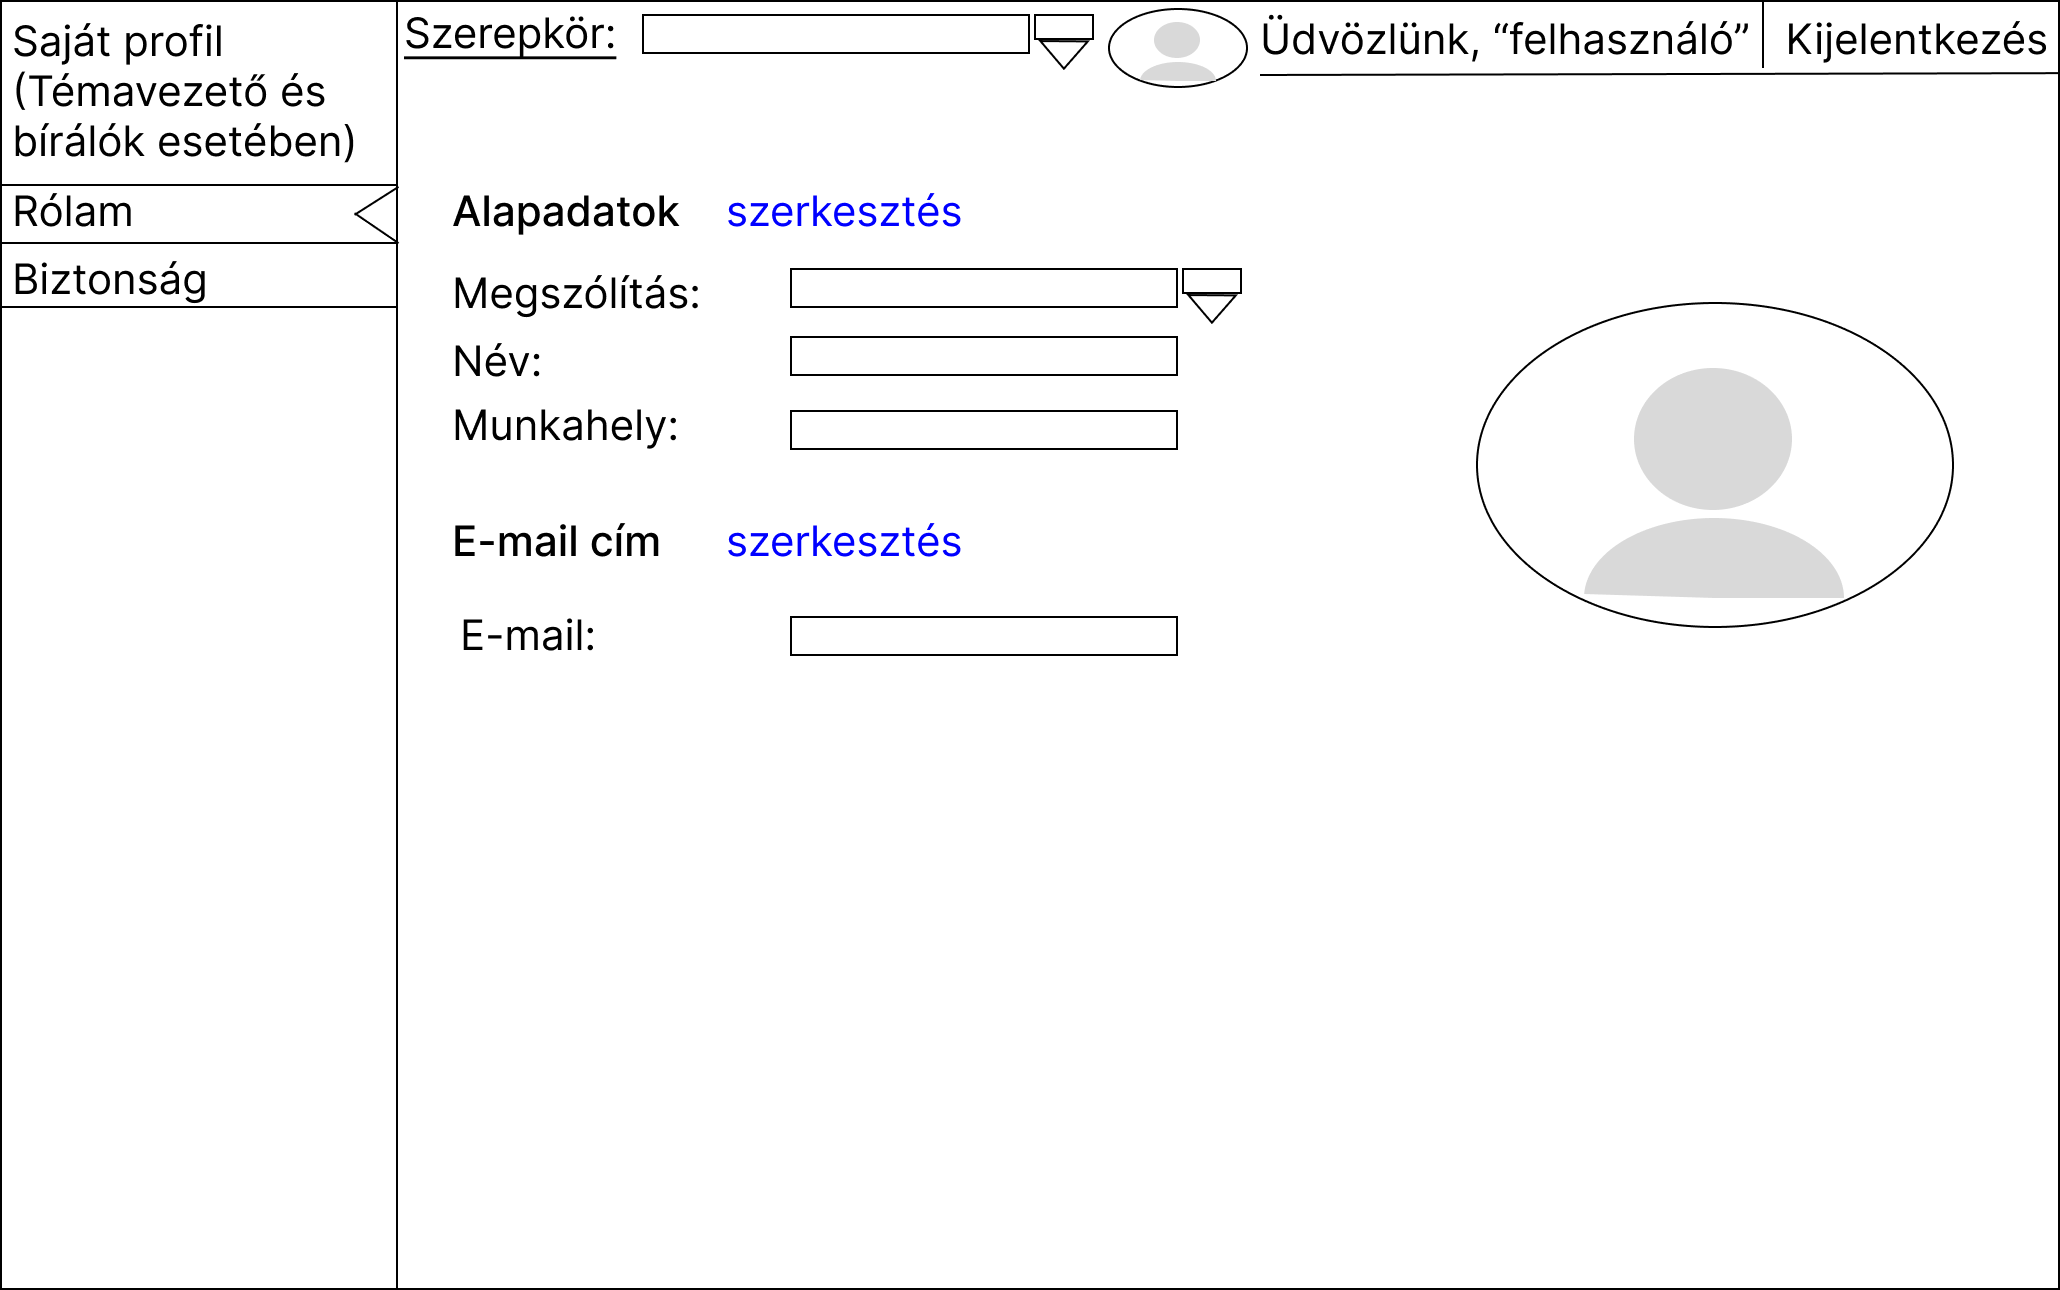
\includegraphics[width=\textwidth]{images/Web_pages/My_Profile.jpg}
	\caption{}
	\label{fig:My_Profile}
\end{figure}

Az *Elnök*, *Bíráló*, *Jegyző*, *Témavezető* saját profilja látható a megadott adatok alapján.    

\subsection{Biztonság (Security)}

\begin{figure}
	\centering
	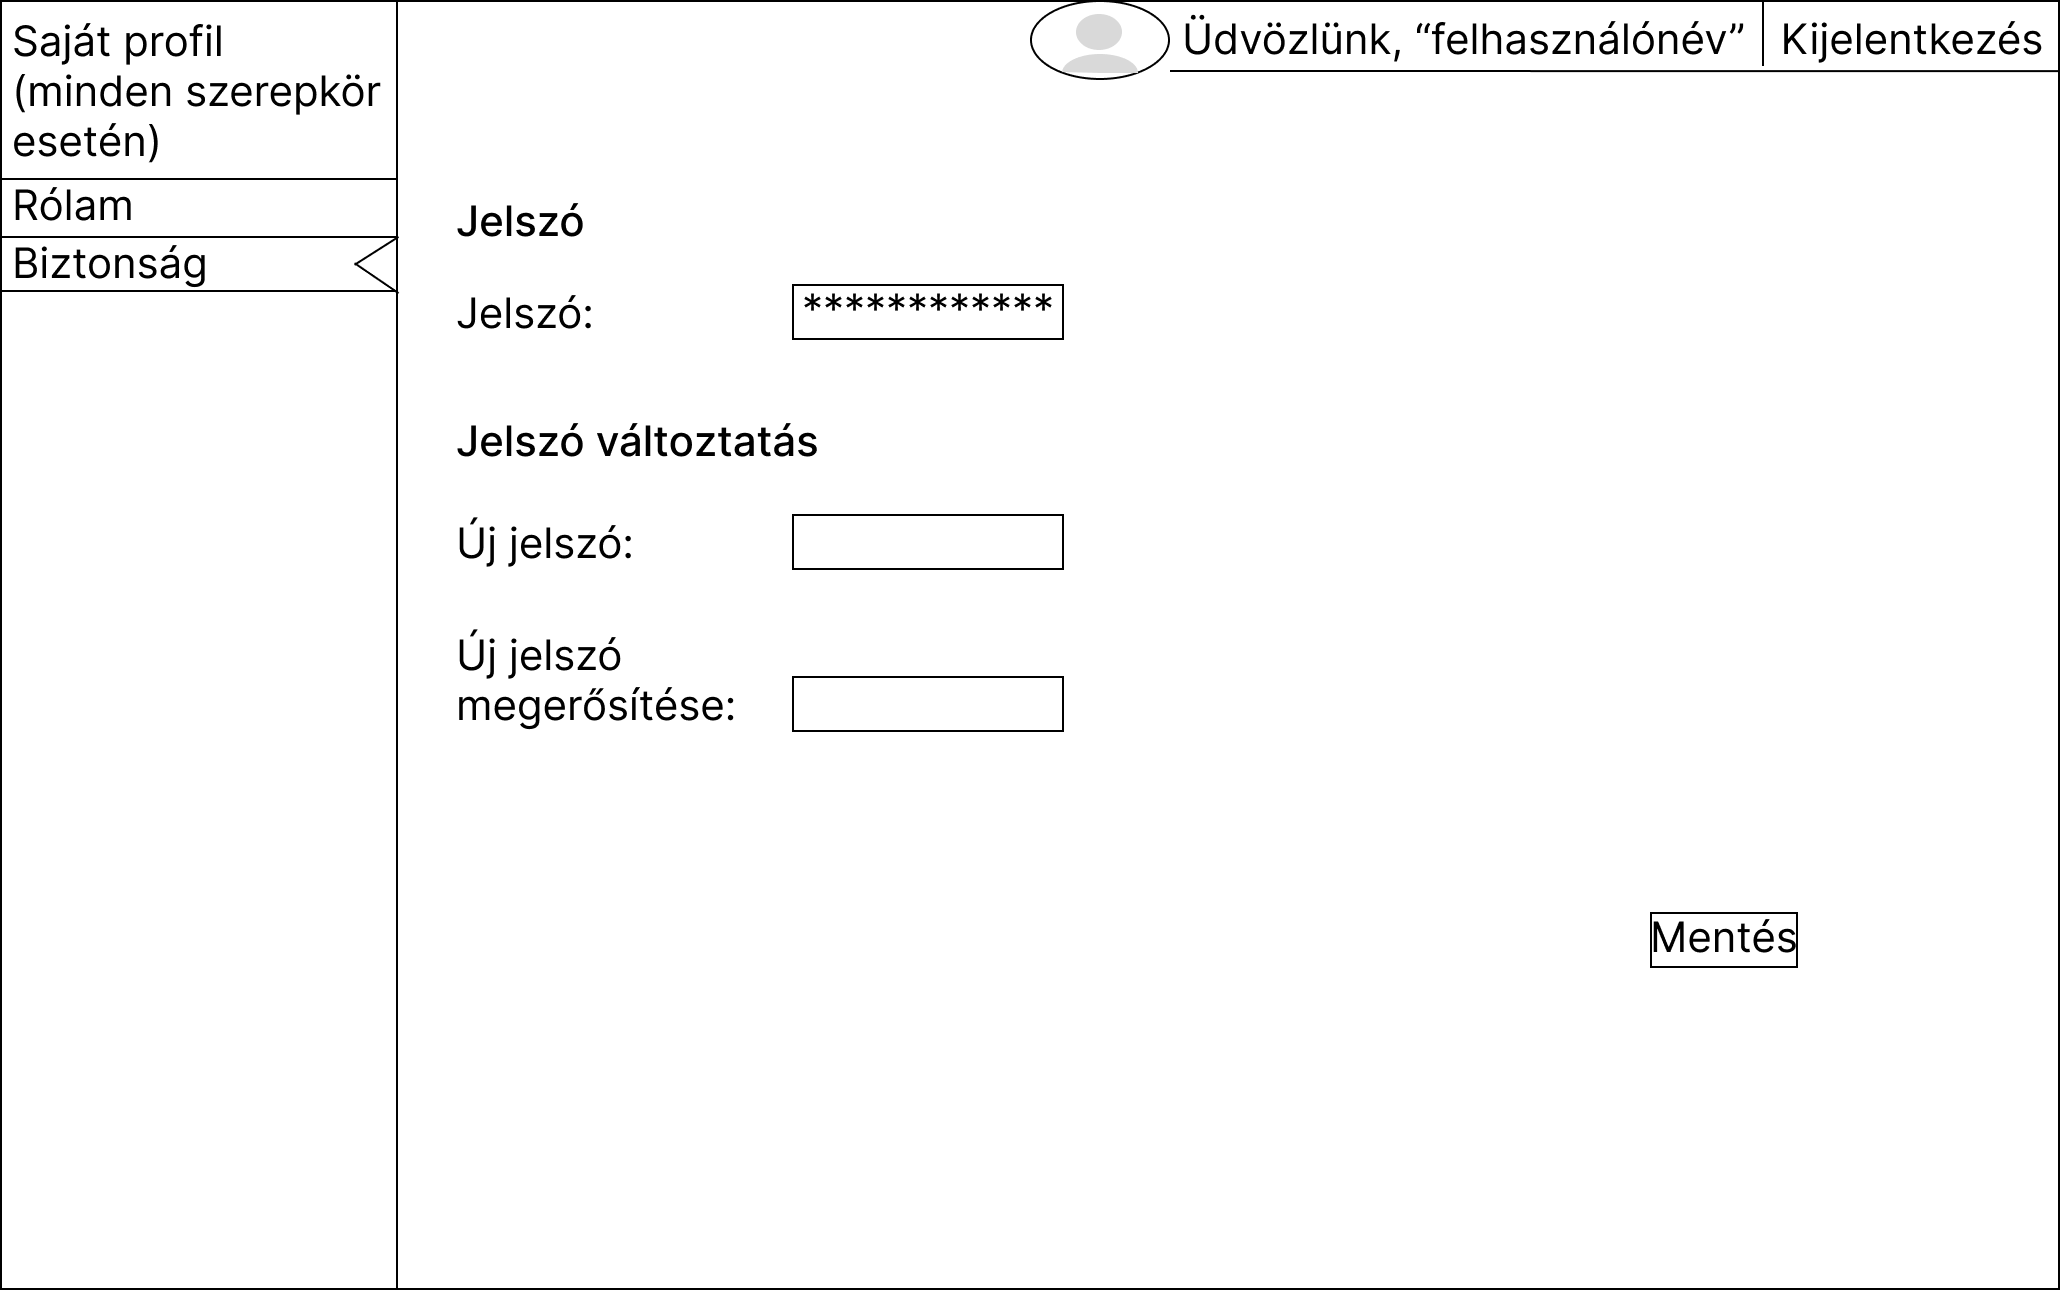
\includegraphics[width=\textwidth]{images/Web_pages/Security.jpg}
	\caption{}
	\label{fig:Security}
\end{figure}

A jelszó változtatás itt történik meg.

\subsection{Történetiséget leíró lap [Hallgató] (History\_Student)}

\begin{figure}
	\centering
	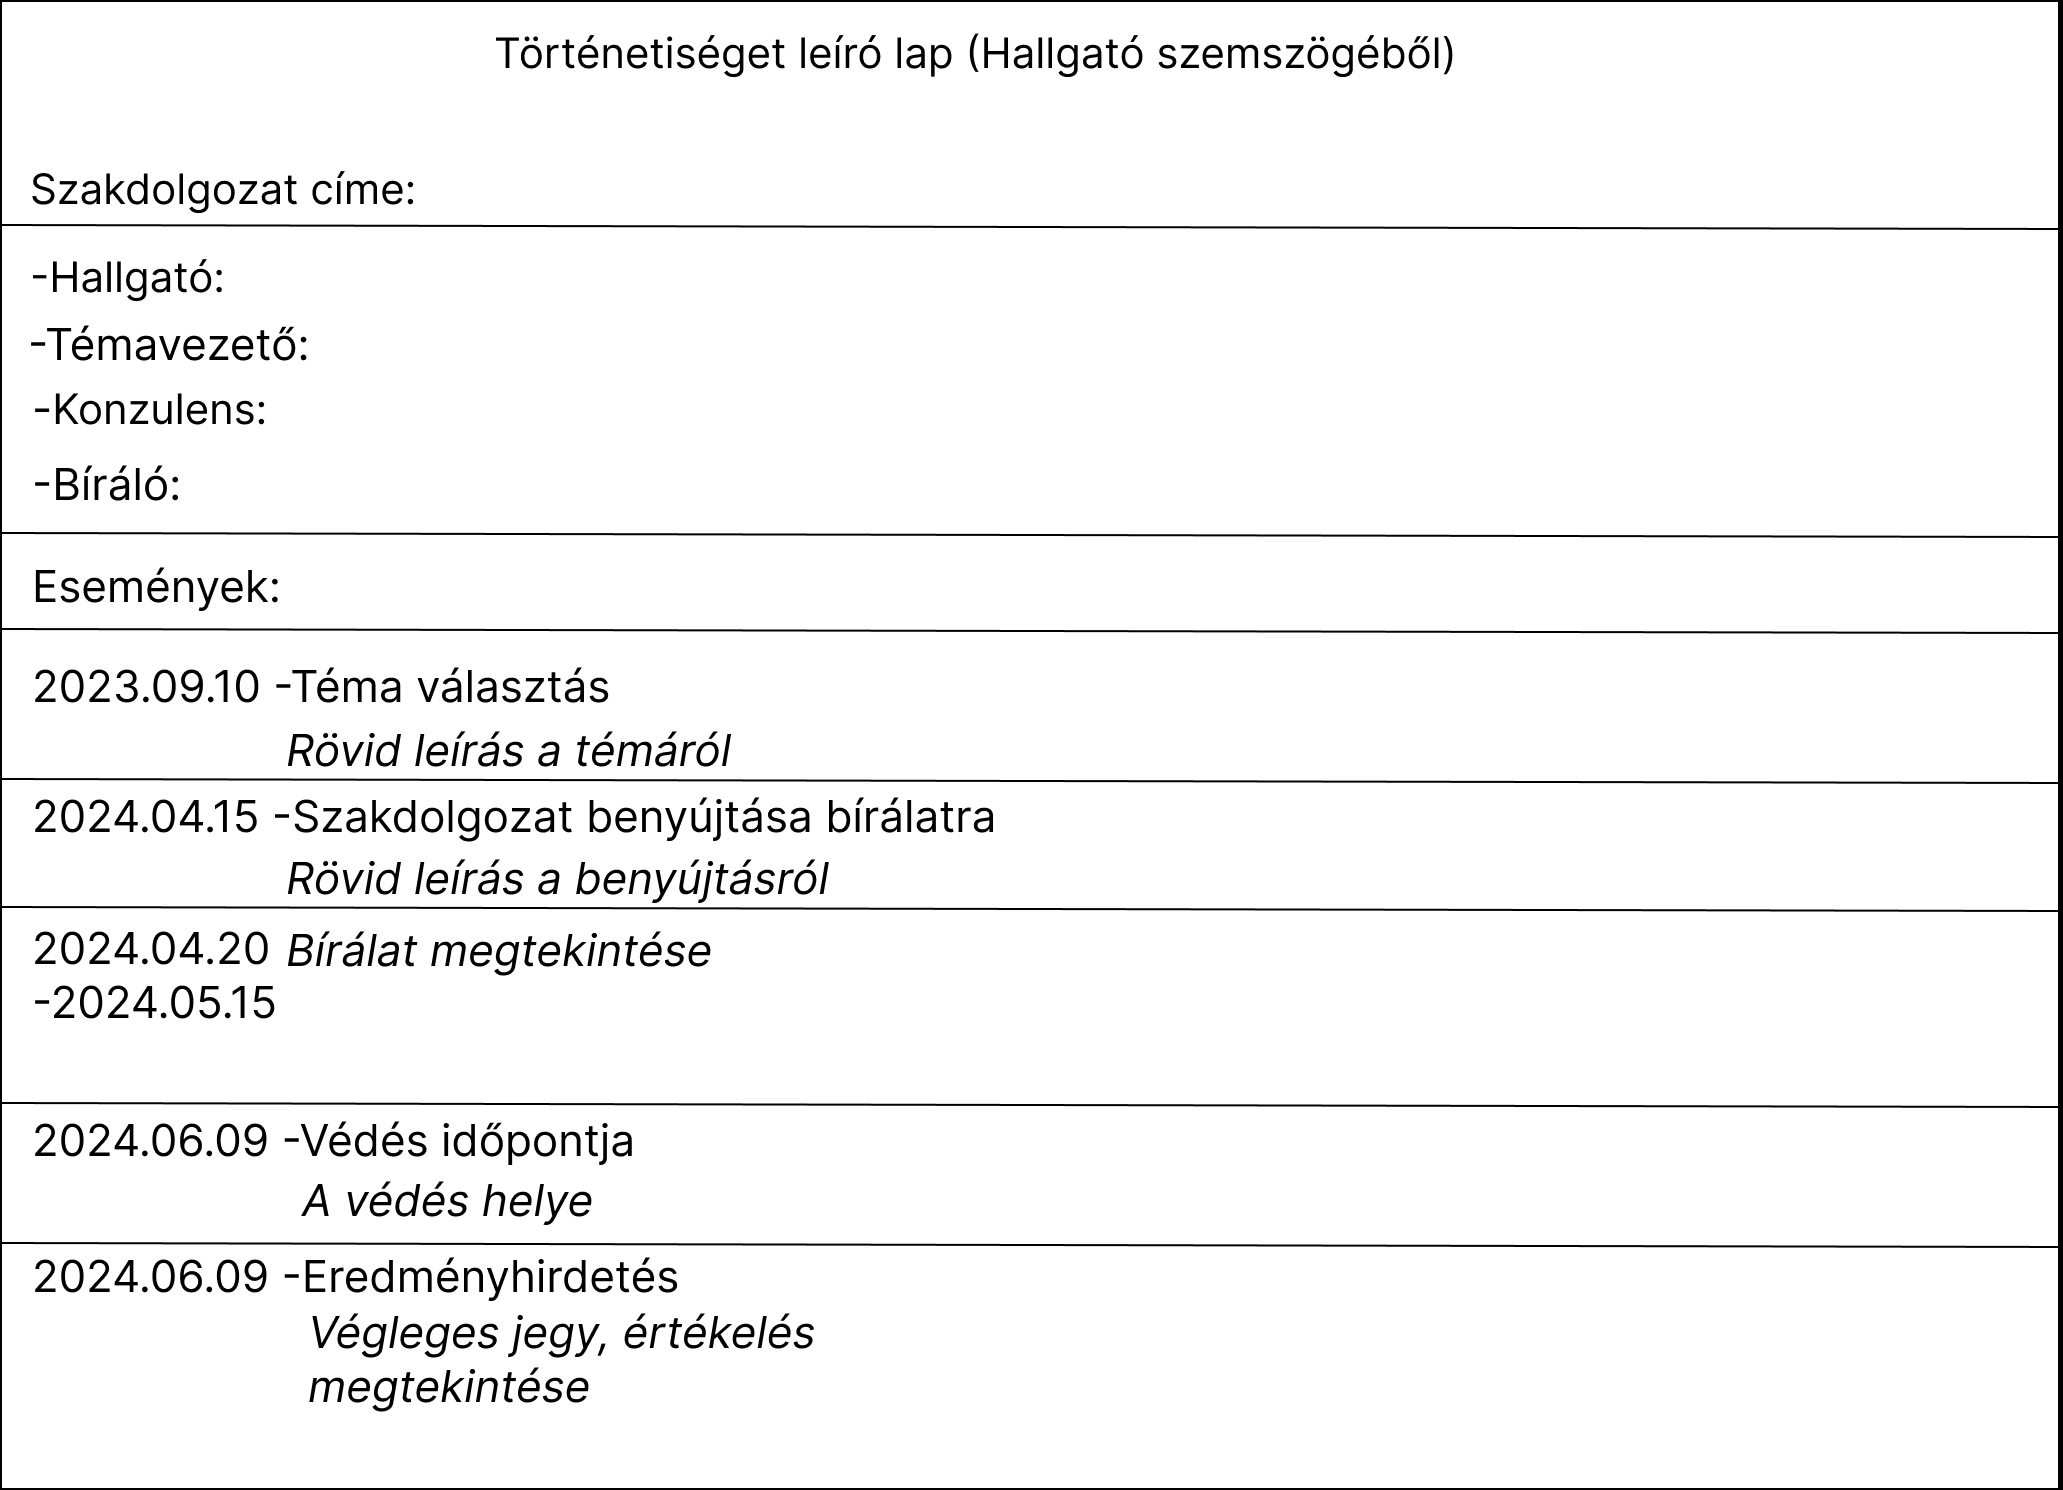
\includegraphics[width=\textwidth]{images/Web_pages/History_Student.jpg}
	\caption{}
	\label{fig:History_Student}
\end{figure}

Egy történetiséget leíró lap látható, amin az egész szakdolgozat procedúra figyelhető meg.

\subsection{Történetiséget leíró lap [Többi szerepkör] (History)}

\begin{figure}
	\centering
	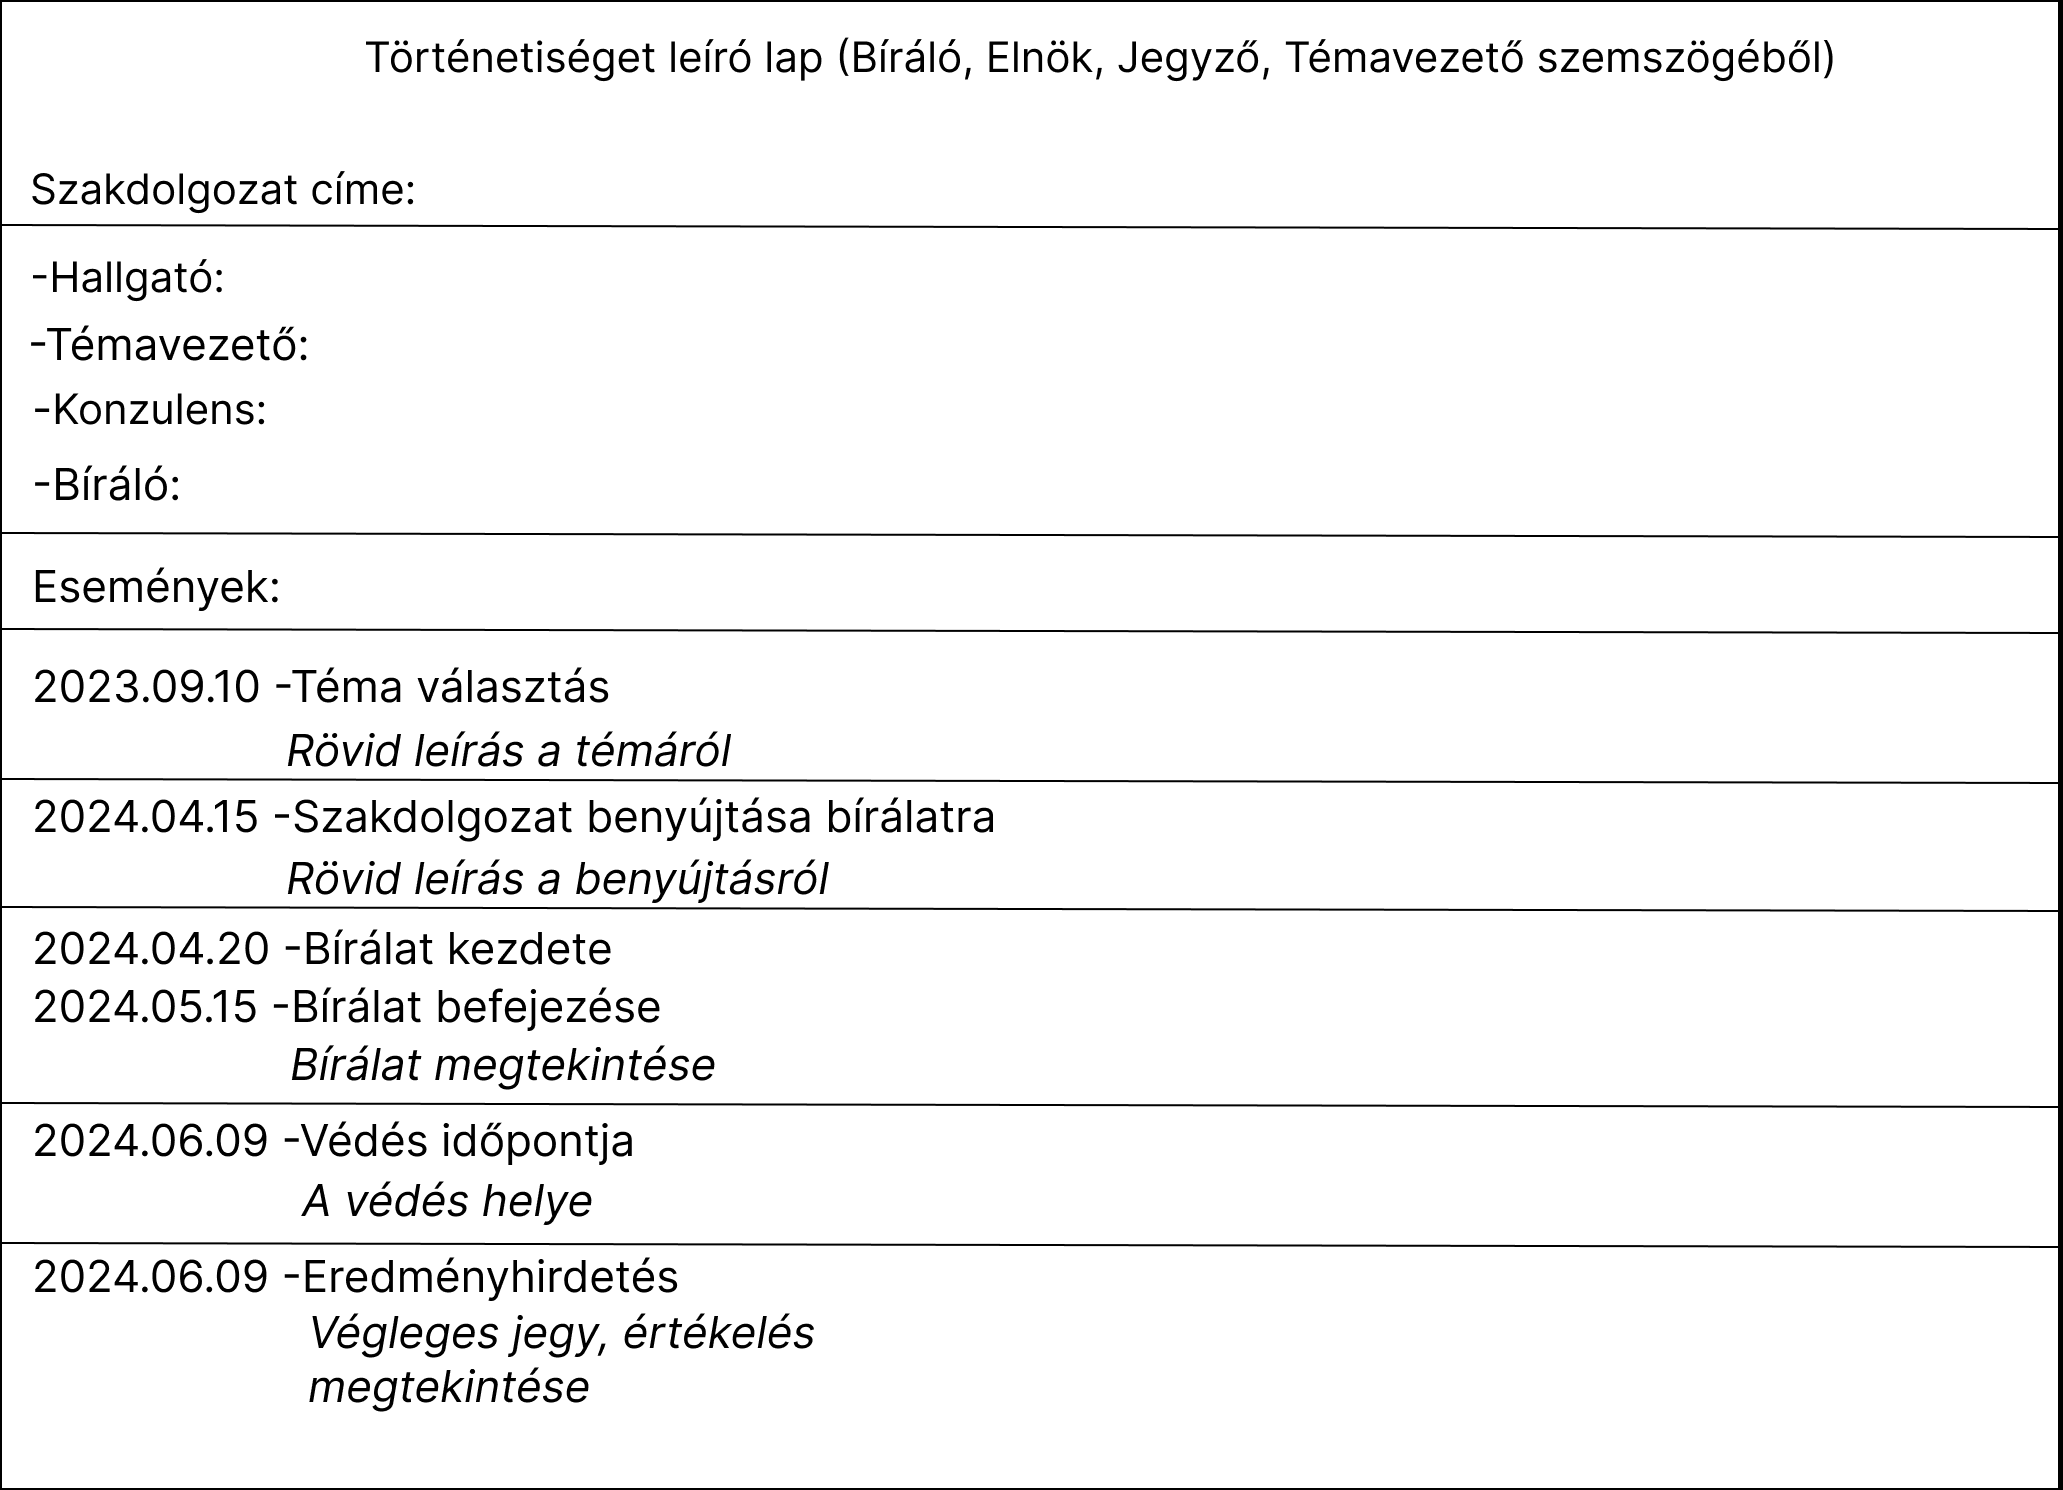
\includegraphics[width=\textwidth]{images/Web_pages/History.jpg}
	\caption{}
	\label{fig:History}
\end{figure}

Egy történetiséget leíró lap látható, amin az egész szakdolgozat procedúra figyelhető meg.

\subsection{Prezentáció feltöltés (Presentation\_Upload)}

\begin{figure}
	\centering
	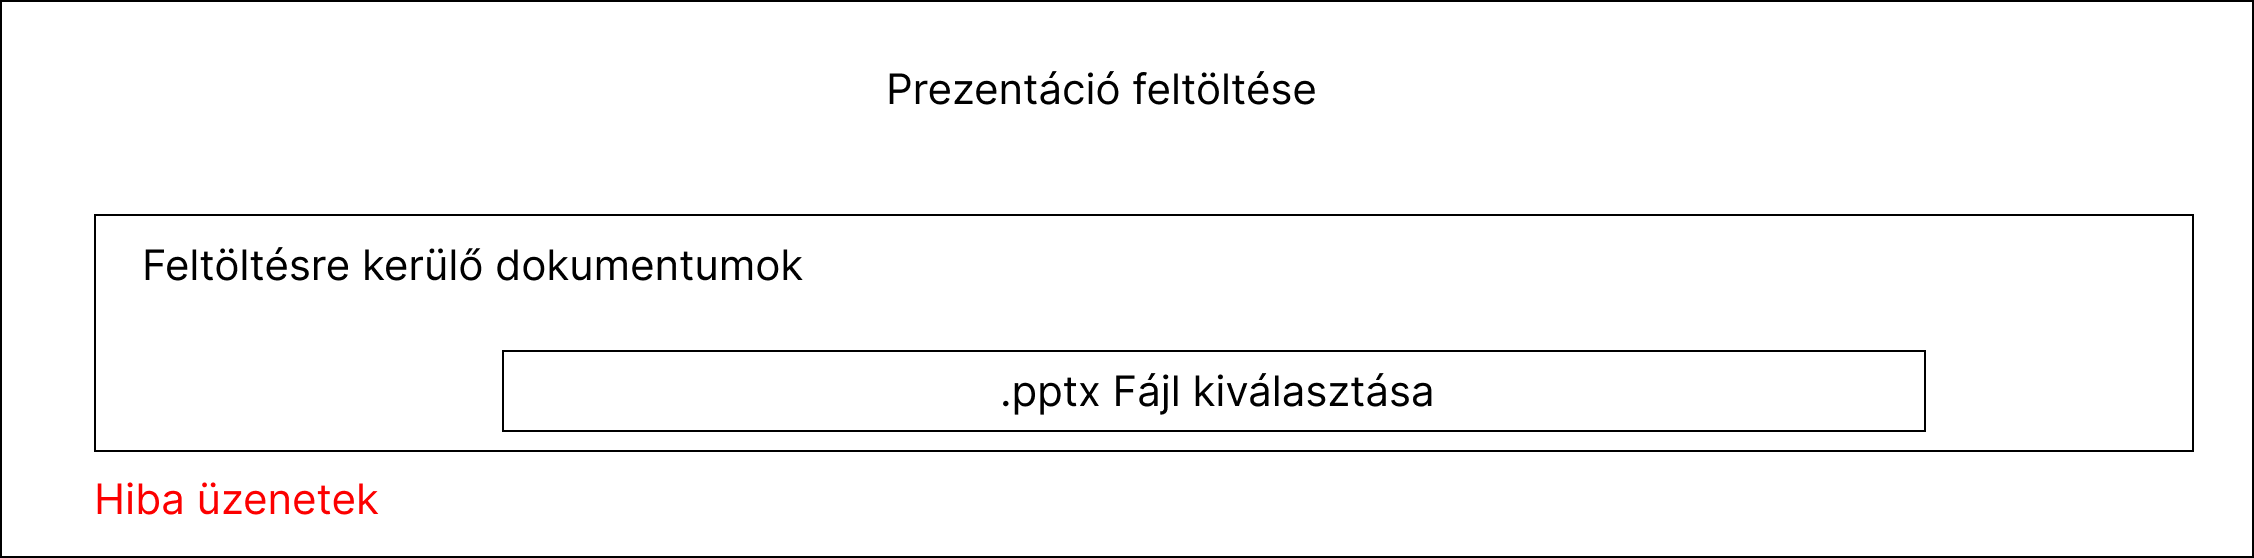
\includegraphics[width=\textwidth]{images/Web_pages/Presentation_Upload.jpg}
	\caption{}
	\label{fig:Presentation_Upload}
\end{figure}

A Záróvizsgához szükséges prezentáció feltöltés itt történik meg.

\subsection{Felhasználói adatok módosítása}

\begin{figure}
	\centering
	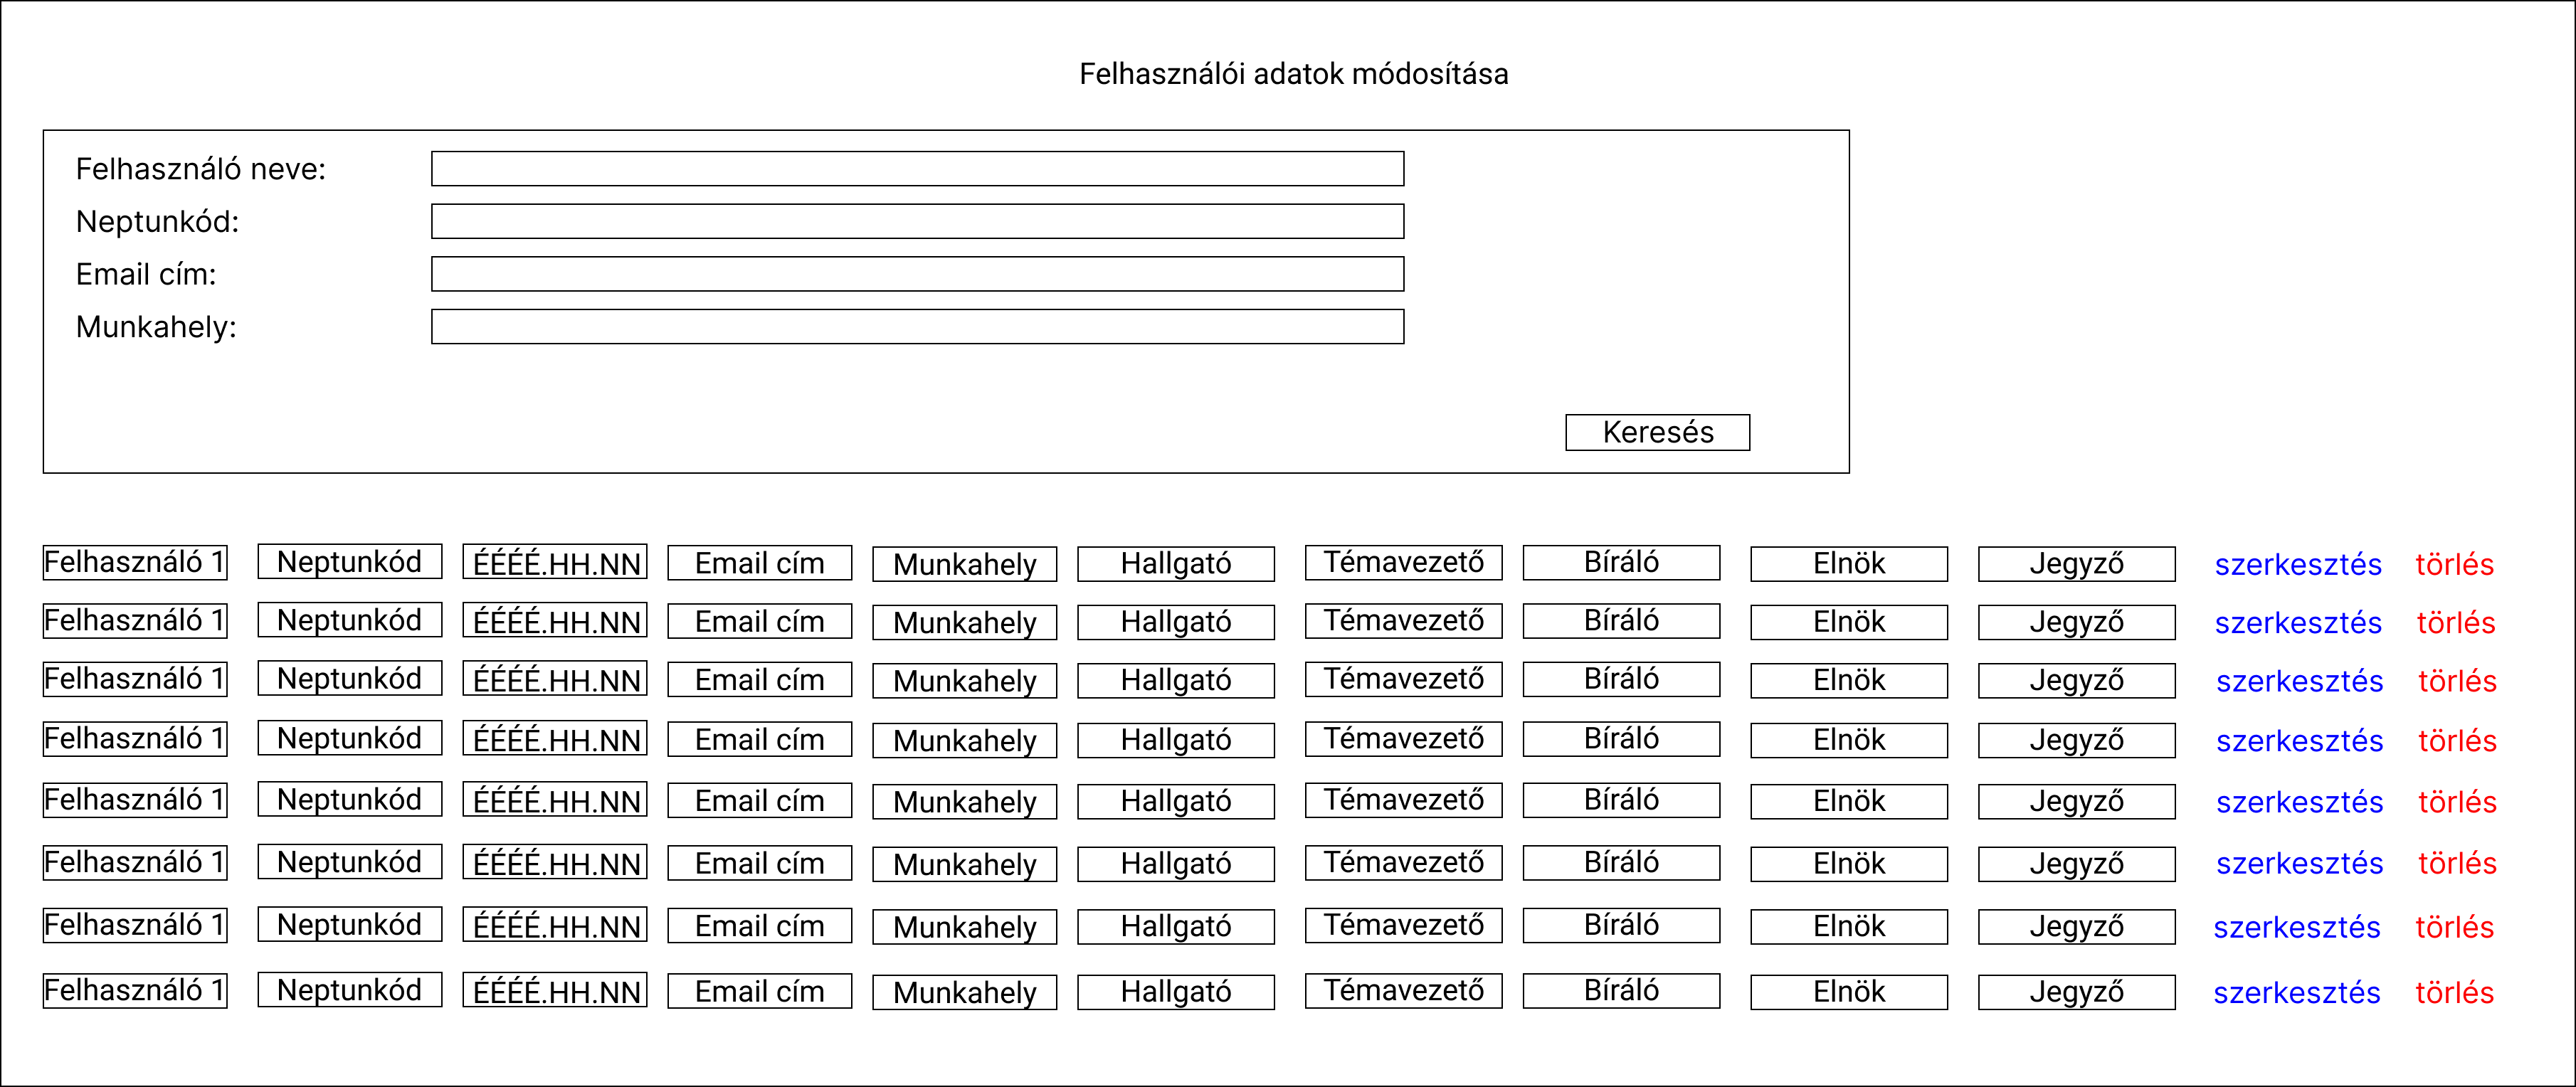
\includegraphics[width=\textwidth]{images/Web_pages/User_Modifiactions.png}
	\caption{}
	\label{fig:User_Modifiactions}
\end{figure}

A felhasználói adatokat illetve jogosultságokat lehet módosítani ezen a lapon.

\section{Lapok közötti átmenetek}

\subsection{Elnök}

\begin{figure}
	\centering
	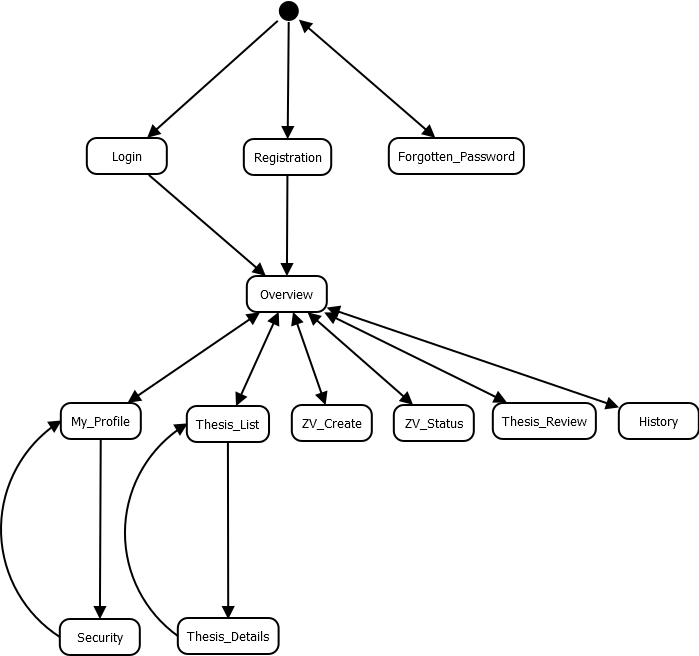
\includegraphics[width=\textwidth]{images/Lapok_kozotti_atmenetek/Elnok.png}
	\caption{}
	\label{fig:Elnok}
\end{figure}

**Leírás**

A fenti ábrán az *Elnök* szemszögéből láthatjuk a rendszert. 
\begin{itemize}
	\item Lehetősége van *Regisztrálni*, *Bejelentkezni*, és *Elfejtett jelszót* kérni. 
	\item A bejelentkezés után rögtön a főoldalra jut a felhasználó. 
	\item Innen lehetősége van megtekinteni a *Saját profilját* és ezen belül a *Biztonság* menüpontot, ahol a jelszót tudja megváltoztatni. 
	\item Ezenkívül hozzáférése lehet a *Szakdolgozatok listázásához* is amin belül az egyes *Szakdolgozatok részleteit* is megjelenítheti a felhasználó. 
	\item Lehetősége van *Záróvizsgát létrehozni*, a *Záróvizsgán kapott jegyeket* elkönyvelni illetve a *Záróvizsga jegyzőkönyvének letöltésére* is. 
	\item Megtekintheti a *Szakdolgozatok státuszát*, a *Bírálatokat* és a *Történetisgéet leíró lapot* is.
\end{itemize}

\subsection{Bíráló}

\begin{figure}
	\centering
	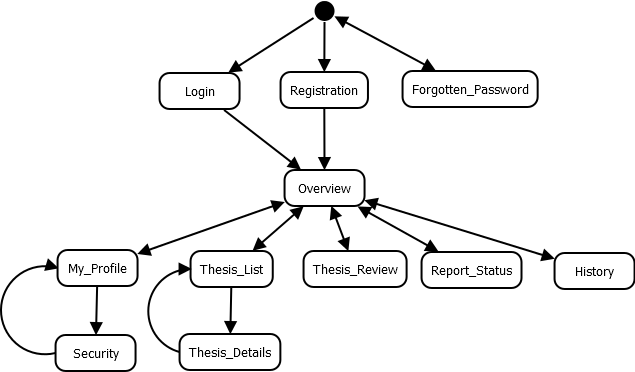
\includegraphics[width=\textwidth]{images/Lapok_kozotti_atmenetek/Biralo.png}
	\caption{}
	\label{fig:Biralo}
\end{figure}

**Leírás**

A fenti ábrán a *Bíráló* szemszögéből láthatjuk a rendszert. 

\begin{itemize}
	\item Lehetősége van *Regisztrálni*, *Bejelentkezni*, és *Elfejtett jelszót* kérni. 
	\item A bejelentkezés után rögtön a főoldalra jut a felhasználó. 
	\item Innen lehetősége van megtekinteni a *Saját profilját* és ezen belül a *Biztonság* menüpontot, ahol a jelszót tudja megváltoztatni. 
	\item Ezenkívül hozzáférése lehet a *Szakdolgozatok listázásához* is amin belül az egyes *Szakdolgozatok részleteit* is megjelenítheti a felhasználó. 
	\item Megtekintheti a *Szakdolgozatok státuszát* és a *Történetiséget leíró lapot* is. Valamint bírálatot írhat a *Szakdolgozat Bírálat* lapon. 
\end{itemize}

\subsection{Jegyző}

\begin{figure}
	\centering
	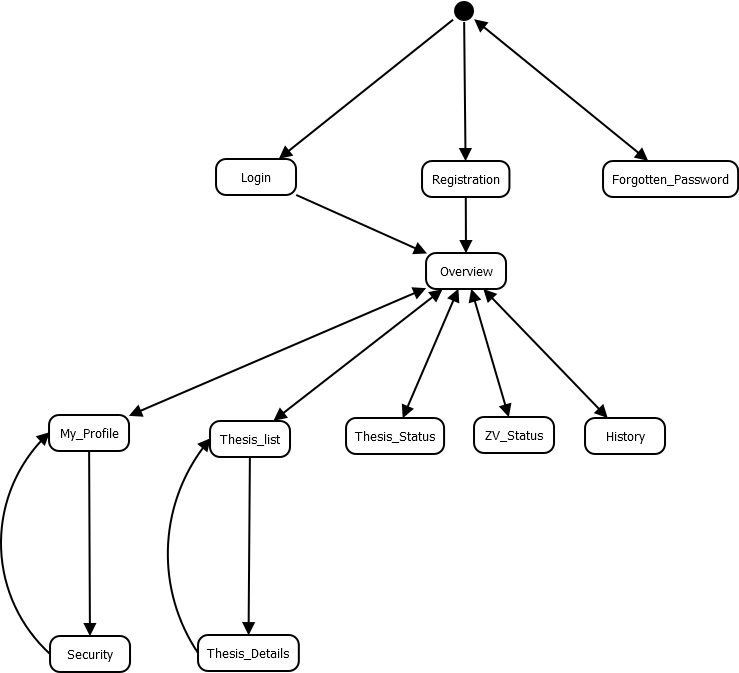
\includegraphics[width=\textwidth]{images/Lapok_kozotti_atmenetek/Jegyzo.png}
	\caption{}
	\label{fig:Jegyzo}
\end{figure}

**Leírás**

A fenti ábrán a *Jegyző* szemszögéből láthatjuk a rendszert. 

\begin{itemize}
	\item Lehetősége van *Regisztrálni*, *Bejelentkezni*, és *Elfejtett jelszót* kérni. 
	\item A bejelentkezés után rögtön a főoldalra jut a felhasználó. 
	\item Innen lehetősége van megtekinteni a *Saját profilját* és ezen belül a *Biztonság* menüpontot, ahol a jelszót tudja megváltoztatni. 
	\item Ezenkívül hozzáférése lehet a *Szakdolgozatok listázásához* is, amin belül az egyes *Szakdolgozatok részleteit* is megjelenítheti a felhasználó. 
	\item Megtekintheti a *Szakdolgozatok státuszát* és a *Történetiséget leíró lapot* is. 
	\item Lehetősége van a *Záróvizsgán kapott jegyek* rögzítésére illetve a *Záróvizsga jegyzőkönyv* letöltésére. 
\end{itemize}

\subsection{Témavezető}

\begin{figure}
	\centering
	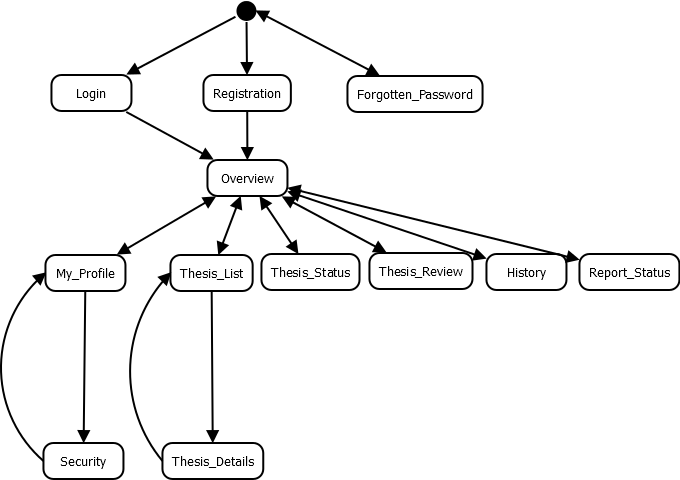
\includegraphics[width=\textwidth]{images/Lapok_kozotti_atmenetek/Temavezeto.png}
	\caption{}
	\label{fig:Temavezeto}
\end{figure}

**Leírás**

A fenti ábrán a *Témavezető* szemszögéből láthatjuk a rendszert.

\begin{itemize}
	\item Lehetősége van *Regisztrálni*, *Bejelentkezni*, és *Elfejtett jelszót* kérni. 
	\item A bejelentkezés után rögtön a főoldalra jut a felhasználó. 
	\item Innen lehetősége van megtekinteni a *Saját profilját* és ezen belül a *Biztonság* menüpontot, ahol a jelszót tudja megváltoztatni. 
	\item Ezenkívül hozzáférése lehet a *Szakdolgozatok listázásához* is, amin belül az egyes *Szakdolgozatok részleteit* is megjelenítheti a felhasználó. 
	\item Megtekintheti a *Szakdolgozatok státuszát* a *Bírálatot*, és a *Történetiséget leíró lapot* is. 
	\item Lehetősége van a *Záróvizsgán kapott jegyek* rögzítésére illetve a *Záróvizsga jegyzőkönyv* letöltésére. 
\end{itemize}

\subsection{Hallgató}

\begin{figure}
	\centering
	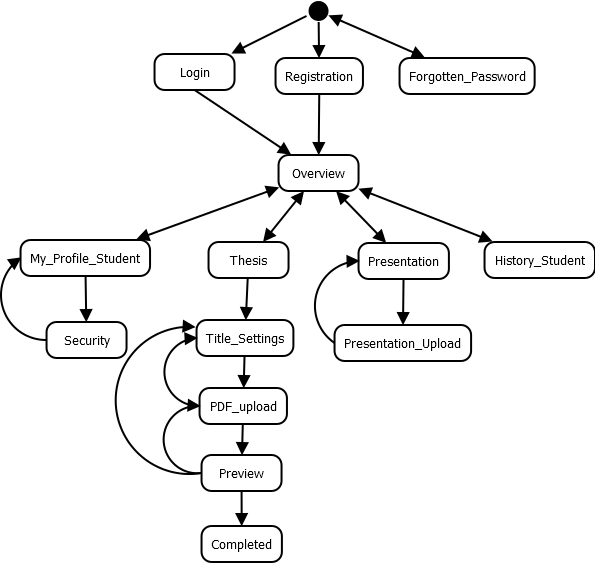
\includegraphics[width=\textwidth]{images/Lapok_kozotti_atmenetek/Hallgato.png}
	\caption{}
	\label{fig:Hallgato}
\end{figure}

**Leírás**

A fenti ábrán a *Hallgató* szemszögéből láthatjuk a rendszert. 

\begin{itemize}
	\item Lehetősége van *Regisztrálni*, *Bejelentkezni*, és *Elfejtett jelszót* kérni. 
	\item A bejelentkezés után rögtön a főoldalra jut a felhasználó. 
	\item Innen lehetősége van megtekinteni a *Saját profilját* és ezen belül a *Biztonság* menüpontot, ahol a jelszót tudja megváltoztatni. 
	\item Ezenkívül hozzáférése lehet a *Szakdolgozatok listázásához* is, amin belül az egyes *Szakdolgozatok részleteit* is megjelenítheti a felhasználó. 
	\item Megtekintheti a *Történetiséget leíró lapot* is. 
	\item Lehetősége van a *Szakdolgozat feltöltésére*, ami különböző fázisokból áll kezdve az *Alapadatok* megadásától a *PDF felöltésen* át az *Előnézetig*. 
	\item A Záróvizsgára készült *prezentációt* is lehetősége van egy külön lapon feltölteni.
\end{itemize}


\section{Összegzés}

\end{document}
